\documentclass[
12pt,
a4paper,
final,
notitlepage,
oneside,
openany,
]{report}

\RequirePackage[l2tabu, orthodox]{nag}

%\usepackage[T1]{fontenc}
%\usepackage[ttdefault=true]{AnonymousPro}
%\renewcommand*\familydefault{\ttdefault} %% Only if the base font of the document is to be typewriter style

%\renewcommand*\ttdefault{txtt}
%\renewcommand*\familydefault{\ttdefault} %% Only if the base font of the document is to be typewriter style
%\usepackage[T1]{fontenc}

\usepackage{tgcursor}
\renewcommand*\familydefault{\ttdefault} %% Only if the base font of the document is to be typewriter style
\usepackage[T1]{fontenc}

%\usepackage[default]{sourcecodepro}
%\usepackage[T1]{fontenc}

%%%%%%%%%%%%%%%%%%%%%%%%%%%%%

%\usepackage{tgcursor}
%\renewcommand*\familydefault{\ttdefault} %% Only if the base font of the document is to be typewriter style

%\renewcommand*\ttdefault{lmvtt}
%\usepackage[T1]{fontenc}
%%\usepackage{courier}
%\renewcommand*\familydefault{\ttdefault}

%\usepackage{courier}
%\renewcommand*\familydefault{\ttdefault} %% Only if the base font of the document is to be typewriter style
%\usepackage[T1]{fontenc}

%\usepackage[scaled]{beramono}
%\renewcommand*\familydefault{\ttdefault} %% Only if the base font of the document is to be typewriter style
%\usepackage[T1]{fontenc}

%\usepackage{FiraMono}
%\renewcommand*\familydefault{\ttdefault} %% Only if the base font of the document is to be typewriter style
%\usepackage[T1]{fontenc}

%\renewcommand*\ttdefault{cmvtt}
%\renewcommand*\familydefault{\ttdefault} %% Only if the base font of the document is to be typewriter style
%\usepackage[T1]{fontenc}

%\renewcommand*\ttdefault{lcmtt}
%\renewcommand*\familydefault{\ttdefault} %% Only if the base font of the document is to be typewriter style
%\usepackage[T1]{fontenc}

%\renewcommand*\ttdefault{lmvtt}
%\renewcommand*\familydefault{\ttdefault} %% Only if the base font of the document is to be typewriter style
%\usepackage[T1]{fontenc}

%\usepackage{nimbusmono}
%\renewcommand*\familydefault{\ttdefault} %% Only if the base font of the document is to be typewriter style
%\usepackage[T1]{fontenc}

%\usepackage[T1]{fontenc}
\usepackage[frenchb]{babel}
\usepackage[utf8]{inputenc}

\usepackage{csquotes}
\usepackage{bold-extra}
\usepackage[
	a4paper,
	includeheadfoot,
	top=0.2cm,
	bottom=1cm,
	left=1.5cm,
	right=1.5cm,
	headheight=1.5cm,
	headsep=1.5cm,
	footskip=2cm,
]{geometry}
\addtolength{\textheight}{1cm}
\setlength{\parskip}{1.5em}
\special{papersize=210mm,297mm}
\setlength{\marginparwidth}{1cm}
\setlength{\marginparsep}{0.3cm}

%\usepackage{showframe} % DEBUG
%%%%%%%%%%%%%%%%%%%%%%%%%%%%%%%%%%%%%%%%%%%%%%%%%%%%%%%%%%%%%%%%%%%%%%%%%%%%%%%%%%%%%%%%%%%%%%%%%%%%%%%%%%%%%%%%%%%%%%%%%%%%%%%%%%%%%%%%%%%%%%%%%%%%%%%%%%%%%%%%%%%%%%%%%%%%%%%%%%%%%%%%
% Define links 
\newcommand{\jplink}{https://www.google.com/url?q=https://fas.org/irp/doddir/dod/jp3_09_3.pdf\&sa=D\&ust=1457816834668000\&usg=AFQjCNEpTH7xDsiu3EjM3xcSy5AatewYrA}
\newcommand{\onethreetwolink}{http://www.132virtualwing.org/}
\newcommand{\thirdwinglink}{http://http://www.3rd-wing.net/}
\newcommand{\dcslink}{http://www.digitalcombatsimulator.com/en/}
%%%%%%%%%%%%%%%%%%%%%%%%%%%%%%%%%%%%%%%%%%%%%%%%%%%%%%%%%%%%%%%%%%%%%%%%%%%%%%%%%%%%%%%%%%%%%%%%%%%%%%%%%%%%%%%%%%%%%%%%%%%%%%%%%%%%%%%%%%%%%%%%%%%%%%%%%%%%%%%%%%%%%%%%%%%%%%%%%%%%%%%%
% Define constants 
\newcommand{\version}{DRAFT 2}
\newcommand{\rgt}{319th Rgt}
\newcommand{\thirdwing}{\href{\thirdwinglink}{3rd Wing}}
%\newcommand{\jp}{\href{\jplink}{JP3-09.3}}
\newcommand{\jp}{\citetitle{jp3093}}
\newcommand{\onethreetwo}{\href{\onethreetwolink}{132nd vWing}}
\newcommand{\docname}{``319th Rgt - Close Air Support - Manuel du pilote''}
\newcommand{\dcs}{\href{\dcslink}{Digital Combat Simulator}}
\newcommand{\inmem}{``In Memoriam Flying Manu''}
\newcommand{\ttitle}{Close Air Support - Manuel du pilote}
\newcommand{\footer}{\rgt{} - \ttitle{} - \version{}}
\newcommand{\ja}{\gls{jtac}/\gls{faca}}
\newcommand{\ipbp}{\gls{ip}/\gls{bp}}
\newcommand{\ipha}{\gls{ip}/\gls{ha}}
%%%%%%%%%%%%%%%%%%%%%%%%%%%%%%%%%%%%%%%%%%%%%%%%%%%%%%%%%%%%%%%%%%%%%%%%%%%%%%%%%%%%%%%%%%%%%%%%%%%%%%%%%%%%%%%%%%%%%%%%%%%%%%%%%%%%%%%%%%%%%%%%%%%%%%%%%%%%%%%%%%%%%%%%%%%%%%%%%%%%%%%%
% Colors
\newcommand{\intlink}{black!70}
\newcommand{\extlink}{blue!80}
%%%%%%%%%%%%%%%%%%%%%%%%%%%%%%%%%%%%%%%%%%%%%%%%%%%%%%%%%%%%%%%%%%%%%%%%%%%%%%%%%%%%%%%%%%%%%%%%%%%%%%%%%%%%%%%%%%%%%%%%%%%%%%%%%%%%%%%%%%%%%%%%%%%%%%%%%%%%%%%%%%%%%%%%%%%%%%%%%%%%%%%%

\usepackage[export]{adjustbox} % loads also graphicx
\usepackage{amssymb}
\usepackage{graphicx}
\graphicspath{ {images/} }

\usepackage{datetime}

\usepackage{import}

\usepackage{xparse}

\usepackage{varwidth}

%\usepackage{parskip}

\usepackage[hyperref=true, backend=bibtex, style=numeric, sorting=ynt]{biblatex}

\addbibresource{main.bib}

\DeclareCiteCommand{\citetitle}
  {\boolfalse{citetracker}%
   \boolfalse{pagetracker}%
   \usebibmacro{prenote}}
  {\ifciteindex
     {\indexfield{indextitle}}
     {}%
   \printtext[bibhyperref]{\printfield[citetitle]{labeltitle}}}
  {\multicitedelim}
  {\usebibmacro{postnote}}
  
\DeclareFieldFormat{url}{\newline\mkbibacro{URL}\addcolon\space\url{#1}}
\renewbibmacro*{url+urldate}{%
 \printfield[url]{url}%   
 \iffieldundef{urlyear}     
 {}     
 {\setunit*{\addspace}%      
 \printtext[urldate]{\printurldate}}}
\usepackage[titles]{tocloft} % Toc, lol, lof, ... styles. http://ctan.cs.uu.nl/macros/latex/contrib/tocloft/tocloft.pdf
\renewcommand{\cftdot}{.}
\renewcommand{\cftpartleader}{\cftdotfill{\cftdotsep}} % for parts
\renewcommand{\cftchapleader}{\cftdotfill{\cftdotsep}} % for chapters
\renewcommand{\cftsecleader}{\cftdotfill{\cftdotsep}}
\setlength\cftbeforechapskip{20pt}
\renewcommand\cftfigafterpnum{\vskip5pt\par}
\renewcommand\cfttabafterpnum{\vskip5pt\par}
\setlength{\cftfignumwidth}{4em}  % Modify number width in LoF
\setlength{\cfttabnumwidth}{4em}
\setlength{\cftchapnumwidth}{2em}
\setlength{\cftsecnumwidth}{3em}
\setlength{\cftsubsecnumwidth}{4em}


% https://tex.stackexchange.com/questions/33841/how-to-modify-the-space-between-the-numbers-and-text-of-sectioning-titles-in-the
\makeatletter
%\renewcommand{\l@section}{\@dottedtocline{1}{1.5em}{2.6em}}
%\renewcommand{\l@subsection}{\@dottedtocline{2}{4.0em}{3.6em}}
\renewcommand{\l@subsubsection}{\@dottedtocline{3}{7em}{5em}}
\makeatother
\usepackage{enumitem}


\def\labelitemi{-}

% Long enum
\newlist{longenum}{enumerate}{8}
\setlistdepth{8}
\setlist[longenum,1]{label=\roman*)}
\setlist[longenum,2]{label=\alph*)}
\setlist[longenum,3]{label=\arabic*)}
\setlist[longenum,4]{label=(\roman*)}
\setlist[longenum,5]{label=(\alph*)}
\setlist[longenum,6]{label=(\alph*)}
\setlist[longenum,7]{label=(\alph*)}
\setlist[longenum,8]{label=(\alph*)}

\newcommand{\elabelindent}{0pt}
\newcommand{\eitemindent}{0em}
\newcommand{\etopsep}{0.5em}
\newcommand{\epartopsep}{0.5em}
\newcommand{\eparsep}{0.5em}
\newcommand{\elabelsep}{1em}


\newcommand{\gene}[3]{
	\begin{longenum}[%
		labelindent=\elabelindent,%
		label*=#1,%
		itemindent=\eitemindent,%
%		leftmargin=!,%
		topsep=\etopsep,%
		itemsep=#2,%
		partopsep=\epartopsep,%
		parsep=\eparsep,%
		labelsep=\elabelsep,%
		leftmargin=#3,
	]
}

\newcommand{\genee}[3]{
	\begin{longenum}[%
		labelindent=\elabelindent,%
		label=#1,%
		itemindent=\eitemindent,%
%		leftmargin=!,%
		topsep=\etopsep,%
		itemsep=#2,%
		partopsep=\epartopsep,%
		parsep=\eparsep,%
		labelsep=\elabelsep,%
		leftmargin=#3,
	]
}
\newcommand{\gener}[3]{
	\begin{longenum}[%
		resume,
		labelindent=\elabelindent,%
		label*=#1,%
		itemindent=\eitemindent,%
%		leftmargin=!,%
		topsep=\etopsep,%
		itemsep=#2,%
		partopsep=\epartopsep,%
		parsep=\eparsep,%
		labelsep=\elabelsep,%
		leftmargin=#3,
	]
}

\newcommand{\geneer}[3]{
	\begin{longenum}[%
		resume,
		labelindent=\elabelindent,%
		label=#1,%
		itemindent=\eitemindent,%
%		leftmargin=!,%
		topsep=\etopsep,%
		itemsep=#2,%
		partopsep=\epartopsep,%
		parsep=\eparsep,%
		labelsep=\elabelsep,%
		leftmargin=#3,
	]
}

% left margin
\newcommand{\llm}       {2em}
\newcommand{\lllm}      {3em}
\newcommand{\llllm}     {4.6em} %4.6
\newcommand{\lllllm}    {2em}
\newcommand{\llllllm}   {2em}
\newcommand{\lllllllm}  {2em}
\newcommand{\llllllllm} {2em}

% itemsep
\newcommand{\ilm}       {1em}
\newcommand{\illm}      {1em}
\newcommand{\illlm}     {1em}
\newcommand{\illllm}    {1em}
\newcommand{\illlllm}   {1em}
\newcommand{\illllllm}  {1em}
\newcommand{\illlllllm} {1em}

%% Leveled enums
%\newcommand{\e}       { \gene  { {\alph*}.    } {\ilm}       {\llm}       }
%\newcommand{\ee}      { \gene  { {\arabic*}   } {\illm}      {\lllm}      }
%\newcommand{\eee}     { \gene  { ({\alph*})   } {\illlm}     {\llllm}     }
%\newcommand{\eeee}    { \genee { ({\arabic*}) } {\illllm}    {\lllllm}    }
%\newcommand{\eeeee}   { \genee { {\Roman*}    } {\illlllm}   {\llllllm}   }
%\newcommand{\eeeeee}  { \genee { ({\roman*})  } {\illllllm}  {\lllllllm}  }
%\newcommand{\eeeeeee} { \genee { ({\arabic*}) } {\illlllllm} {\llllllllm} }
%
%
%% resume
%\newcommand{\re}       {\gener  { {\alph*}.    } {\ilm}       {\llm}       }
%\newcommand{\ree}      {\gener  { {\arabic*}   } {\illm}      {\lllm}      }
%\newcommand{\reee}     {\gener  { ({\alph*})   } {\illlm}     {\llllm}     }
%\newcommand{\reeee}    {\geneer { ({\arabic*}) } {\illllm}    {\lllllm}    }
%\newcommand{\reeeee}   {\geneer { {\Roman*}    } {\illlllm}   {\llllllm}   }
%\newcommand{\reeeeee}  {\geneer { ({\roman*})  } {\illllllm}  {\lllllllm}  }
%\newcommand{\reeeeeee} {\geneer { ({\arabic*}) } {\illlllllm} {\llllllllm} }
%
%% terminate
%\newcommand{\ed}{\end{longenum}}

% Environment
%\newenvironment{e1}[1][\ilm]       {\gene  { {\alph*}.    } {#1} {\llm}       } {\end{longenum}}
%\newenvironment{e2}[1][\illm]      {\gene  { {\arabic*}   } {#1} {\lllm}      } {\end{longenum}}
%\newenvironment{e3}[1][\illlm]     {\gene  { ({\alph*})   } {#1} {\llllm}     } {\end{longenum}}
%\newenvironment{e4}[1][\illllm]    {\genee { ({\arabic*}) } {#1} {\lllllm}    } {\end{longenum}}
%\newenvironment{e5}[1][\illlllm]   {\genee { {\Roman*}    } {#1} {\llllllm}   } {\end{longenum}}
%\newenvironment{e6}[1][\illllllm]  {\genee { ({\roman*})  } {#1} {\lllllllm}  } {\end{longenum}}
%\newenvironment{e7}[1][\illlllllm] {\genee { ({\arabic*}) } {#1} {\llllllllm} } {\end{longenum}}
%\newenvironment{e8}{\eeeeeeee}{\ed}


%%%%%%%%%%%%%%%%%%%%%%%%%%%%%%%%%%%%%%%%%%%%%%%%%%%%%%%%%%%%%%%%%%%%%%%%%%%%%%%%%
% Glossary enum
\newlist{glossaryenum}{enumerate}{8}
\setlistdepth{8}
\setlist[glossaryenum,1]{label=\roman*)}
\setlist[glossaryenum,2]{label=\alph*)}
\setlist[glossaryenum,3]{label=\arabic*)}
\setlist[glossaryenum,4]{label=(\roman*)}
\setlist[glossaryenum,5]{label=(\alph*)}
\setlist[glossaryenum,6]{label=(\alph*)}
\setlist[glossaryenum,7]{label=(\alph*)}
\setlist[glossaryenum,8]{label=(\alph*)}

\newcommand{\glene}[2]{
	\begin{glossaryenum}[%
		labelindent=0pt,%
		label*=#1,%
		itemindent=0em,%
%		leftmargin=!,%
		topsep=0em,%
		itemsep=0em,%
		partopsep=0em,%
		parsep=0em,%
		labelsep=1em,%
		leftmargin=2.2em,
	]
}

\newcommand{\gle}{
	\glene{{\alph*}.}{2em}
}

\newcommand{\gled}{
	\end{glossaryenum}
}

\newcommand{\eskip}{
	\\ \vskip0.5em
}

\newcommand{\itemt}[2]{
	\item \textbf{#1} \par #2
}
\newenvironment{e1} [1][\ilm]       {\gene   { {\alph*}.    } {#1} {\llm}       } {\end{longenum}}
\newenvironment{e2} [1][\illm]      {\gene   { {\arabic*}   } {#1} {\lllm}      } {\end{longenum}}
\newenvironment{e3} [1][\illlm]     {\gene   { ({\alph*})   } {#1} {\llllm}     } {\end{longenum}}
\newenvironment{e4} [1][\illllm]    {\genee  { ({\arabic*}) } {#1} {\lllllm}    } {\end{longenum}}
\newenvironment{e5} [1][\illlllm]   {\genee  { {\Roman*}    } {#1} {\llllllm}   } {\end{longenum}}
\newenvironment{e6} [1][\illllllm]  {\genee  { ({\roman*})  } {#1} {\lllllllm}  } {\end{longenum}}
\newenvironment{e7} [1][\illlllllm] {\genee  { ({\arabic*}) } {#1} {\llllllllm} } {\end{longenum}}
\newenvironment{re1}[1][\ilm]       {\gener  { {\alph*}.    } {#1} {\llm}       } {\end{longenum}}
\newenvironment{re2}[1][\illm]      {\gener  { {\arabic*}   } {#1} {\lllm}      } {\end{longenum}}
\newenvironment{re3}[1][\illlm]     {\gener  { ({\alph*})   } {#1} {\llllm}     } {\end{longenum}}
\newenvironment{re4}[1][\illllm]    {\geneer { ({\arabic*}) } {#1} {\lllllm}    } {\end{longenum}}
\newenvironment{re5}[1][\illlllm]   {\geneer { {\Roman*}    } {#1} {\llllllm}   } {\end{longenum}}
\newenvironment{re6}[1][\illllllm]  {\geneer { ({\roman*})  } {#1} {\lllllllm}  } {\end{longenum}}
\newenvironment{re7}[1][\illlllllm] {\geneer { ({\arabic*}) } {#1} {\llllllllm} } {\end{longenum}}
\usepackage{float}
\newcommand{\efig}[2]{ \begin{figure}[H] \includegraphics[width=\textwidth]{#1.png} \caption{#2} \label{#1} \end{figure} }
\usepackage[pagestyles]{titlesec}

%%%%%%%%%%%%%%%%%%%%%%%%%%%%%%%%%%%%%%%%%%%%%%%%%%%%%%%%%%%%%%%%%%%%%%%%%%%%%%%%%%%%%%%%%%%%%%%%%%%%%%%%%%%%%%%%%%%%%%%%%%%%%%%%%%%%%%%%%%%%%%%%%%%%%%%%%%%%%%%%
%% Chapter title formatting ----------------------------------------------
%\titleformat
%{\chapter} % command
%[block] % shape
%%{\huge\bfseries} % format
%{\huge\ttseries\filcenter\textsc}%format
%{\thechapter.} % label
%{1ex} % sep
%{
%%    \rule{\textwidth}{1pt}
%%	\null
%%    \vspace{1em}
%    \textsc
%%    \centering
%} % before-code
%[
%%\vspace{-0.5ex}%
%%\rule{\textwidth}{0.3pt}
%] % after-code
\titleformat{\chapter}[display]
{\scshape\bfseries\Large}
{ %\Huge\textsc{\chaptertitlename}
\hfill\fontsize{120}{70}\selectfont\color{lightgray}\textsc{\textbf{\thechapter}}}
{-2ex}
{\filleft\fontsize{50}{70}\selectfont\scshape}
[\vspace{0ex}]

\titlespacing*{\chapter}{0pt}{50pt}{40pt}

% Section title formatting ----------------------------------------------
\titleformat{\section}[block]
{\Large\bfseries}
{\thesection.}{0.5em}{\textsc}

% Subsection title formatting -------------------------------------------
\titleformat{\subsection}[block]
{\large}%{\large\bfseries}
{\thesubsection.}{0.5em}{\textsc}

% Subsection title formatting -------------------------------------------
\titleformat{\subsubsection}[block]
{\normalsize}%{\normalsize\bfseries}
{\thesubsubsection.}{0.5em}{\textsc}
\usepackage{fancyhdr}
% Define default styles ------------------------------------------------------------
\newcommand{\deflhead}{\minipage[b]{.9\linewidth}\small\leftmark{} \\ \rightmark{}\endminipage}
\newcommand{\defrhead}{
\includegraphics[width=1cm]{images/319th.png}}
\newcommand{\deflfoot}{\footnotesize \footer}
\newcommand{\defrfoot}{\thepage}
% -----------------------------------------------------------------------------------
\fancypagestyle{default}{%
	\fancyhf{}% Clear header and footer
	\fancyhead[L]{\deflhead{}}
	\fancyhead[R]{\defrhead{}}
	\fancyfoot[L]{\deflfoot{}}% Custom footer
	\fancyfoot[R]{\defrfoot{}}% Custom footer
	\renewcommand{\headrulewidth}{0.4pt}% Line at the header visible
	\renewcommand{\footrulewidth}{0.4pt}% Line at the footer visible
}

% Redefine the plain page style
\fancypagestyle{plain}{%
	\fancyhf{}% Clear header and footer
	\fancyhead[L]{\deflhead{}}
	\fancyhead[R]{\defrhead{}}
	\fancyfoot[L]{\deflfoot{}}% Custom footer
	\fancyfoot[R]{\defrfoot{}}% Custom footer
	\renewcommand{\headrulewidth}{0.4pt}% Line at the header visible
	\renewcommand{\footrulewidth}{0.4pt}% Line at the footer visible
}

\fancypagestyle{intro}{%
	\fancyhf{}% Clear header and footer
	\fancyhead[L]{\minipage[b]{.9\linewidth}\large\leftmark \endminipage}
	%\fancyhead[L]{\rightmark{}}
	\fancyhead[R]{\defrhead{}}
	\fancyfoot[L]{\deflfoot{}}% Custom footer
	\fancyfoot[R]{\defrfoot{}}% Custom footer
	\renewcommand{\headrulewidth}{0.4pt}% Line at the header visible
	\renewcommand{\footrulewidth}{0.4pt}% Line at the footer visible
}

\fancypagestyle{annexes}{%
	\fancyhf{}% Clear header and footer
	\fancyhead[L]{\minipage[b]{.9\linewidth}\large Annexe \thechapter{}. \leftmark \endminipage}
	%\fancyhead[L]{\rightmark{}}
	\fancyhead[R]{\defrhead{}}
	\fancyfoot[L]{\deflfoot{}}% Custom footer
	\fancyfoot[R]{\defrfoot{}}% Custom footer
	\renewcommand{\headrulewidth}{0.4pt}% Line at the header visible
	\renewcommand{\footrulewidth}{0.4pt}% Line at the footer visible
}

\fancypagestyle{logoonly}{%
	\fancyhf{}
	%\fancyfoot[L]{\deflfoot{}}% Custom footer
	\fancyhead[R]{\defrhead{}}% Custom footer
	\renewcommand{\headrulewidth}{0pt}% Line at the header visible
	\renewcommand{\footrulewidth}{0pt}% Line at the header visible
}

\pagestyle{default}


\usepackage[
    font=footnotesize,
    labelfont={sf, bf},
    margin=1cm
]{caption}

\captionsetup{font={scriptsize, tt}, labelfont={sc, it},textfont={it, sc}}
\usepackage{listings}

\lstset{
	frame=left, frame=bottom,
	extendedchars=false,
	escapeinside="",
	numbers=left,
	basicstyle=\small\normalfont\sffamily,% the size of the fonts that are used for the code
	stepnumber=1,% the step between two line-numbers. If it is 1 each line will be numbered
	numbersep=0cm,% how far the line-numbers are from the code
	tabsize=2,% tab size in blank spaces
	extendedchars=true, %
	breaklines=true,% sets automatic line breaking
	captionpos=b, % sets the caption-position to top
	mathescape=true,
	%stringstyle=\color{white}\ttfamily,
	showspaces=false,
	showtabs=false,
	xleftmargin=5pt,
	xrightmargin=5pt,
	framexleftmargin=5pt,
	framexrightmargin=5pt,
	framexbottommargin=5pt,
	framextopmargin=5pt,
	showstringspaces=false
}
 
\renewcommand\lstlistingname{Exemple}
\renewcommand\lstlistlistingname{Liste des exemples}
\usepackage{booktabs}
\usepackage{tabularx}
%\usepackage{pdfpages}

\newcolumntype{R}{>{\raggedleft\arraybackslash}X|}
%
\usepackage{array}
\usepackage[many]{tcolorbox}

\newcommand{\customcoloredbox}[2]{
	%\parbox[c]{\linewidth}{
		\begin{tcolorbox}%
		[%
			box align=center,
			colframe=gray!10!#1,%
			boxrule=1pt,%
			leftrule=3mm,%
			colback=#1!20!white%
		]%
		#2%
		\end{tcolorbox}%
	%}
}



\newcommand{\customnotebox}[2]{%
	\begin{tcolorbox}%
	[%
		box align=center,
		colback=#1!5!white,%
		colframe=#1!75!black,%
		fonttitle=\bfseries,%
		colbacktitle=#1!85!black,%
		enhanced,%
		attach boxed title to top center={yshift=-2mm},%
		title=Note%
	]%
	#2%
	\end{tcolorbox}%
}


\newcommand{\note}[1]{\customnotebox{blue}{#1}}
\newcommand{\important}[1]{\customcoloredbox{red}{#1}}
\newcommand{\useful}[1]{\customcoloredbox{blue}{#1}}
\newcommand{\remark}[1]{\customcoloredbox{gray}{#1}}
\newcommand{\emptypage}{
\null  % Empty line
\nointerlineskip  % No skip for prev line
\vfill
\let\snewpage \newpage
\let\newpage \relax
\begin{center}
Page intentionnellement vide
\end{center}
\let \newpage \snewpage
\vfill 
\break % page break
}
% Invisible section
\newcommand\invisiblesection[1]{%
    \refstepcounter{section}%
    \phantomsection%
    \addcontentsline{toc}{section}{\protect\numberline{\thesection}#1}%
    \sectionmark{#1}%
    \markboth{\textsc{{\Large #1}}}{}
}

% Invisible unnumbered section
\newcommand\invisibleunnumberedsection[1]{%
    %\addcontentsline{toc}{section}{\protect{\thesection}#1}%
    \phantomsection%
    \addcontentsline{toc}{section}{\protect\numberline{}#1}
    \sectionmark{#1}%
    \markboth{\textsc{{\Large #1}}}{}
}

% Invisible chapter
\newcommand\invisiblechapter[1]{%
    \refstepcounter{chapter}%
    \phantomsection%
    \addcontentsline{toc}{chapter}{\protect\numberline{\thechapter}#1}%
    \chaptermark{#1}%
    %\chapter{#1}
    \markboth{\textsc{{\Large #1}}}{}
}

% Invisible unnumbered chapter
\newcommand\invisibleunnumberedchapter[1]{%
    %\addcontentsline{toc}{section}{\protect{\thesection}#1}%
    \phantomsection%
    \addcontentsline{toc}{chapter}{\protect\numberline{}#1}
    \chaptermark{#1}%
    %\chapter*{#1}
    \markboth{\textsc{{\Large #1}}}{}
}
%%%%%%%%%%%%%%%%%%%%%%%%%%%%%%%%%%%%%%%%%%%%%%%%%%%%%%%%%%%%%%%%%%%%%%%%%%%%%%%%%%%%%%%%%%%%%%%%%%%%%%%%%%%%%%%%%%%%%%%%%%%%%%%%%%%%%%%%%%%%%%%%%%%%%%%%%%%%%%%%
% Set space between paragraphs -----------------------------------------------------
\newlength{\defaultparskip}% Save parskip
\newlength{\defaultparindent}% Save parindent
\setlength{\defaultparskip}{\parskip}% save the value
\setlength{\defaultparindent}{\parindent}% save the value
\newlength{\currentparskip}% Save parskip
\newlength{\currentparindent}% Save parindent
%%%%%%%%%%%%%%%%%%%%%%%%%%%%%%%%%%%%%%%%%%%%%%%%%%%%%%%%%%%%%%%%%%%%%%%%%%%%%%%%%%%%%%%%%%%%%%%%%%%%%%%%%%%%%%%%%%%%%%%%%%%%%%%%%%%%%%%%%%%%%%%%%%%%%%%%%%%%%%%%
% One page
\newcommand{\addstretch}[1]{\addtolength{#1}{\fill}}
\newenvironment{onepage}
  {
	\setlength{\currentparskip}{\parskip}% save the value
	\setlength{\currentparindent}{\parindent}% save the value
	\newpage\flushbottom
	\addstretch{\baselineskip}
	\addstretch{\abovedisplayskip}
	\addstretch{\abovedisplayshortskip}
	\addstretch{\belowdisplayskip}
	\addstretch{\belowdisplayshortskip}
	\setlength{\parskip}{0pt}
}
{
	\newpage
	\setlength{\parskip}{\currentparskip}%
	\setlength{\parindent}{\currentparindent}%
}




\newenvironment{smini}%
{%
\setlength{\currentparskip}{\parskip}% save the value
\setlength{\currentparindent}{\parindent}% save the value
\noindent\begin{minipage}[c][\textheight][s]{\linewidth}%
\baselineskip=1\baselineskip plus 1fill% stretch as much as needed
\lineskip=0pt plus 1fill% just for safety
\setlength{\parskip}{\currentparskip}%
%\setlength{\parindent}{\currentparindent}%
}% restore the value
{\end{minipage}}%

\newenvironment{mini}%
{%
\setlength{\currentparskip}{\parskip}% save the value
\setlength{\currentparindent}{\parindent}% save the value
\begin{minipage}[s][\textheight]{\linewidth}%
\baselineskip=1\baselineskip plus 1fill% stretch as much as needed
\lineskip=0pt plus 1fill% just for safety
\setlength{\parskip}{\currentparskip}%
%\setlength{\parindent}{\currentparindent}%
}% restore the value
{\end{minipage}}%

\newenvironment{imini}%
{%
\setlength{\currentparskip}{\parskip}% save the value
\setlength{\currentparindent}{\parindent}% save the value
\noindent%
\begin{minipage}[s][\textheight]{\linewidth}%
\baselineskip=1\baselineskip plus 1fill% stretch as much as needed
\lineskip=0pt plus 1fill% just for safety
\setlength{\parskip}{\currentparskip}%
\setlength{\parindent}{\currentparindent}%
}% restore the value
{\end{minipage}}%

%%%%%%%%%%%%%%%%%%%%%%%%%%%%%%%%%%%%%%%%%%%%%%%%%%%%%%%%%%%%%%%%%%%%%%%%%%%%%%%%%%%%%%%%%%%%%%%%%%%%%%%%%%%%%%%%%%%%%%%%%%%%%%%%%%%%%%%%%%%%%%%%%%%%%%%%%%%%%%%%



\usepackage{tikz}
\usetikzlibrary{calc}
\usetikzlibrary{fit}
\usetikzlibrary{shapes}
\usetikzlibrary{positioning}
\usetikzlibrary{matrix, backgrounds}

\tikzset{my arrow/.style={-latex, thick, orange}}
\tikzstyle{process} = [rectangle, minimum width=2cm, minimum height=2cm, text centered, text width=2.2cm, fill=orange!60]
\usepackage[french]{todonotes}

%\renewcommand{\todo}[1]{\todo[inline]{#1}}
\usepackage{soul}% http://ctan.org/pkg/soul
\sodef\spaceout{}{0pt plus 1fil}{.4em plus 1fil}{0pt}

\usepackage[
	colorlinks=true,
	urlcolor=\extlink,
	filecolor=\extlink,
	linkcolor=\intlink,
	citecolor=\intlink,
	bookmarks=true,
]{hyperref}

\usepackage{cleveref}
\usepackage{nameref}

\crefname{annex}{Annexe}{Annexes}
%\crefalias{annex}{Annexe}{Annexes}

\newcommand{\fullref}[1]{%
Cfr. \cref{#1}: %
\nameref{#1}%
}

\newcommand{\smallref}[1]{%
\cref{#1}: %
\nameref{#1}%
}

\renewcommand{\ref}{\fullref}
\newcommand{\smallref}[1]{\cref{#1}: \nameref{#1}}
\newcommand{\fullref}[1]{Cfr. \smallref{#1}}
\renewcommand{\ref}{\fullref}
\usepackage[acronym,toc,nopostdot]{glossaries}
% command: makeglossaries %
%\renewcommand\glossarytitle{}
\makeglossaries

\newcommand{\newgls}[4]{% 1: abbrev 2: full name 3: ref 4: desc
	\newglossaryentry{#3g}{%
		name={#1},%
		description={#4}%
	}%
	\newglossaryentry{#3}{%
		type=\acronymtype,%
		name={#1},%
		description={#2},%
		first={#2 (#1)\glsadd{#3g}},%
		see=[Explication:]{#3g}%
	}%
}

\newgls{FFA}{Free Fire Area}{ffa}{%
Une zone spécifique dans laquelle le tir est autorisé sans coordination préalable
}

\newgls{FSCL}{Fire Support Coordination Line}{fscl}{%
Mesure de coordination du tir mise en place par le \gls{gc} au sein d'une zone d'opération; tout tir au delà de cette ligne doit être préalablement coordonné avec le \gls{gc} local, et avant laquelle tout tir doit être coordonnée avec le \gls{gc} qui a établi la FSCL
}

\newgls{CFL}{Coordinated Firing Line}{cfl}{%
Ligne au delà de laquelle le tir est autorisé sans coordination avec l'échelon supérieur
}

\newgls{NAI}{Named Area of Interest}{nai}{%
Zone particulière à laquelle on aura attribué un nom (ou qui porte déjà un nom, par ex. une ville)
}

\newgls{TAI}{Target Area of Interest}{tai}{%
Zone cible particulière
}

\newgls{AOF}{Azimuth Of Fire}{aof}{%
Direction dans laquelle tire une unité
}

\newgls{IFF}{Identitification Friend or Foe}{iff}{%
Système électronique embarqué permettant d'interroger à distance un appareil et de l'identifier comme ami
}

\newgls{PID}{Positive Identification}{pid}{%
Identification visuelle, électronique, \gls{iff} ou autre obtenue par l'observation et l'analyse des caractéristiques de la cible
}

\newgls{CP}{Contact Point}{cp}{%
Point sur lequel, lorsqu'elle arrive dessus, une unité est censée en contacter une autre
}

\newgls{POF}{Priorities Of Fire}{pof}{%
Priorités de tir
}

\newgls{COE}{Concept Of Employment}{coe}{%
Façon d'employer quelque chose
}

\newgls{JIPOE}{Joint Intelligence Preparation of the Operational Environment}{jipoe}{%
Le processus analytique par lequel les organisations de renseignement produisent des estimations et autres pour aider au processus de prise de décision pas le \gls{jfc}
}

\newgls{CAS request}{CAS request}{req}{%
Une requête \gls{cas} est une demande de \gls{cas} émise par une unité alliée au sol pour obtenir un support aérien. Ce support peut être planifié à l'avance (``Pre-planned \gls{cas}''), ou immédiat (``On-call \gls{cas}'')
}

\newgls{OPLAN}{Operational Plan}{oplan}{%
\parbox{\linewidth}{1. Tout plan pour la conduite d'une opération militaire préparée en réponse à une situation effective ou prévue.}\glvs{}
\parbox{\linewidth}{2. Un plan Joint complet et détaillé contenant la description complète du \gls{conops}, toutes les annexes d'application au plan, et une chronologie prévue de l'emploi de la force et du déploiement}
}

\newgls{TOS}{Time On Station}{tos}{%
Heure d'arrivée prévue sur la zone cible, de patrouille, sur l'objectif, etc.
}

\newgls{ACM}{Airspace Control Measure}{acm}{%
Directive visant à rendre l'utilisation des unités aériennes efficaces et aptes à remplir leur mission tout permettant le transit sécurisé dans l'espace aérien
}

\newgls{ACA}{Airspace Coordination Area}{aca}{%
Un bloc tridimensionnel d'espace aérien se trouvant dans une zone cible, défini par l'autorité appropriée, dans lequel les appareils alliés sont normalement hors de danger d'être touché par un tir ami provenant du sol (artillerie, principalement, ou Kakane, parfois)
}


\newgls{DAS}{Deep Air Support}{das}{%
Le DAS englobe le \gls{ai}, le \gls{ar} et le \gls{scar}, trois types de missions qui, à l'inverse du \gls{cas}, sont dirigées contre les unités ennemies au sol qui ne trouvent pas à proximité des forces au sol alliées
}

\newgls{AI}{Air Interdiction}{ai}{%
\parbox{\linewidth}{L'interdiction aérienne consiste à utiliser une unité aérienne pour attaquer des cibles ennemies tactiques au sol qui ne trouvent pas à proximité de forces au sol alliées}\glvs{}
\parbox{\linewidth}{L'interdiction diffère du \gls{cas} en cela qu'elle ne soutient pas directement les opérations des forces au sol, et qu'elle n'est pas coordonnée aussi étroitement avec ces dernières}\glvs{}
\parbox{\linewidth}{A la différence du bombardement stratégique, l'interdiction n'est pas une campagne aérienne à part entière, de par son objectif ultime qui reste le soutien des forces au sol alliées, là où le bombardement stratégique vise à défaire l'ennemi par la puissance aérienne uniquement}\glvs{}
\parbox{\linewidth}{L'objectif de l'interdiction est de retarder, perturber ou détruire les forces ennemies ou la logistique en route vers la zone de combat avant qu'elles en deviennent un facteur pour les forces alliées. Même à ce degré, une distinction est faite entre l'interdiction stratégique et l'interdiction tactique; l'interdiction stratégique est prévue à grande échelle et sur le long terme, là où l'interdiction tactique agit de manière rapide et localisée}
}

\newgls{SCAR}{Air Interdiction}{scar}{%
\glvs{}
\parbox{\linewidth}{Le SCAR est une mission dont l'objectif est l'acquisition et le rapportage de cible pour le \gls{das}. Les missions SCAR coordonnent et peuvent marquer les cibles pour les missions \gls{ai}, ou repérer précisément les cibles pour les missions \gls{ar}. Le SCAR ne doit pas être confondu avec le \gls{faca}}\glvs{}
\parbox{\linewidth}{\gle
	\item Le SCAR ne nécessite pas une qualification \gls{faca} pour le \gls{tac} des missions \gls{das}
	\item Le SCAR fournit des cibles, des positions, des descriptions, des informations quant à la météo ou la menace
	\item Le SCAR peut fournir la marque mais pas l'autorisation de tir
	\item Le SCAR confirme ou découvre des menaces air-sol
	\item Le SCAR assiste à l'établissement de la \gls{bda}
	\item Le SCAR diffère d'une mission de reconnaissance de par le fait qu'il découvre les cibles et coordonne leurs destruction, et qu'il sera typiquement armé et équipé de manière à améliorer la désignation des cibles
\gled}\glvs{}
\parbox{\linewidth}{Le SCAR est particulièrement utile dans un environnement riche en cible. Un appareil en mission SCAR qui se trouve à court de munitions peut continuer sa mission}
}

\newgls{AR}{Armed Reconnaissance}{ar}{%
\parbox{\linewidth}{La reconnaissance armée est utilisée quand la position exacte de la cible est inconnue, et que le pilote devra localiser et engager les cibles potentielles pour accomplir l'objectif. Ces missions impliquent que l'appareil sera exposé pendant de longues période en territoire ennemi, à la recherche de cibles potentielles}\glvs{}
\parbox{\linewidth}{\gle
	\item Identifier des cibles dont la position est inconnue et les engager avant qu'elles ne deviennent un facteur
	\item Empêcher l'ennemi d'effectuer un mouvement non détecté ou d'accéder à une zone clef
	\item Fournir un avertissement précoce quant à la position et aux intentions de l'ennemi
	\item Empêcher ou dégrader la mobilité de l'ennemi
	\item Reconnaître une grande étendue de terrain qui serait moins facilement explorée par les forces au sol amies
	\item Attaquer des cibles dont la destruction doit se faire rapidement (menaces en mouvement vers le front, par exemple)
	\item Soutien lors des opérations de sécurité, soit comme unité de soutien du support ou comme couverture, garde ou écran principal
\gled}
}

\newgls{BAI}{Battlefield Air Interdiction}{bai}{%
Cfr AI
}

\newgls{COMSEC}{Communications Security}{comsec}{%
Tout ce qui a trait à la sécurisation des communications alliées
}

\newgls{FSCM}{Fire Support Coordination Measure}{fscm}{%
Directive mise en place pour coordonner le tir de support (artillerie)
}

\newgls{FSCOORD}{Fire Support Coordinator}{fscoord}{%
Officier en charge de la coordination du tir de support (artillerie)
}

\newgls{COA}{Course Of Action}{coa}{%
Ligne de conduite, façon de faire
}

\newgls{5-Line}{5-Line}{5l}{%
La 5-Line est une version résumée de la \gls{9l}, réservée aux hélicoptères, et centrées sur les forces alliées
}

\newgls{9-Line}{9-Line}{9l}{%
Format standard du briefing donné par le J-TAC/FAC(A)
}

\newgls{FLOT}{Forward Line Of Troops}{flot}{%
Ligne de front, là où les troupes alliées sont les plus avancées
}

\newgls{FRAGO}{Fragmentary Order}{frago}{%
Forme abrégée de l'\gls{opord} publiée journellement
}

\newgls{BOC}{Bombs On Coordinates}{boc}{%
Méthode d'attaque consistant à attaquer la cible au moyen d'une munition intelligente sur des coordonnées, parfois sans jamais acquérir la cible. La méthode d'attaque BOC implique de rentrer \textbf{directement} les coordonnées de la cible dans le système lors du \gls{cas} brief, et d'effectuer le read-back de la ligne 6 en \textbf{relisant les coordonnées entrées dans le système}
}

\newgls{HMCS}{Helmet Mounted Cueing System}{hmcs}{%
Système de visée monté sur le casque (HMS)
}

\newgls{FLIR}{Forward Looking Infrared}{flir}{%
Équipement embarqué permettant de voir en infrarouge devant l'appareil
}

\newgls{FOV}{Field Of View}{fov}{%
Champ de vision
}

\newgls{IDF}{Indirect Fire}{idf}{%
Feu indirect, c-à-d artillerie
}

\newgls{TRP}{Target Reference Point}{trp}{%
Point de référence cible (NAV TGT dans le PVI800)
}

\newgls{BOT}{Bombs On Target}{bot}{%
Méthode d'attaque consistant à attaquer après l'avoir acquise visuellement ou via les senseurs embarqués
}

\newgls{stack}{stack}{stack}{%
Mise en attente des appareils de manière sécurisée
}

\newgls{GPS}{Global Positionning System}{gps}{%
Système permettant d'obtenir les coordonnées d'un point sur la terre au moyen d'une constellation de satellites
}

\newgls{LRF}{Laser Range Finder}{lrf}{%
Laser servant à calculer une distance
}

\newgls{JDAM}{Joint Direct Attack Munition}{jdam}{%
Un JDAM est un kit qui convertit une bombe lisse en bombe guidée \gls{gps}
}

\newgls{MSL}{Mean Sea Level}{msl}{%
Niveau moyen de la mer
}

\newgls{HVT}{High Value Target}{hvt}{%
Cible de grande importance
}

\newgls{CSAR}{Combat Search and Rescue}{csar}{%
Recherche et sauvetage de combat
}

\newgls{OPCON}{Operationnal Control}{opcon}{%
Entité qui exerce le contrôle opérationnel (stratégique), par opposition au contrôle tactique (\gls{tacon})
}

\newgls{SEAD}{Suppression of Ennemy Air Defence}{sead}{%
Aussi appelé ``Wild Weasel'', ou ``Iron Hand''. Action visant à neutraliser les défenses anti-aériennes ennemies, pas uniquement les \glspl{sam} ou \glspl{aaa}, mais également les \glspl{ewr} et le \gls{ccc}. Cette action peut être effectuée au moyen d'armement, ou de moyens de guerre électronique
}

\newgls{CID}{Combat Identification}{cid}{%
Capacité de différencier les cibles potentielles, mobiles ou fixes, dans de grandes zones, comme amies, ennemies ou neutre, dans un temps très court, avec un grand degré de certitude, et à la distance suffisante, pour permettre les décisions d'emploi de la force
}

\newgls{AOD}{Air Operation Directive}{aod}{%
Directive émise par le \gls{jfacc} concernant la conduite des opération aériennes%
}

\newgls{ROE}{Rule of Engagement}{roe}{%
Décrit les circonstances, les conditions, la manière et la proportion dans lesquelles l'usage de la force est autorisé%
}

\newgls{TGO}{Terminal Guidance Operation}{tgo}{%
Action de fournir aux appareils ou aux armes des informations supplémentaires relatives à la cible par la voix, l'électronique, les communications visuelles ou des moyens mécaniques%
}

\newgls{TAC}{Terminal Attack Control}{tac}{%
Autorité qui contrôle la manœuvre %
}

\newgls{BDA}{Battle Damage Assessment}{bda}{%
Évaluation des dégâts infligés à la cible, ou aux cibles, suite à un engagement%
}

\newgls{FAC(A)}{Forward Air Controller}{faca}{%
Un pilote spécialement qualifié qui contrôle, depuis les airs, d'autres appareils engagés en opération de \gls{cas}%
}

\newgls{J-TAC}{Joint Terminal Attack Controller}{jtac}{%
Un membre du personnel qualifié qui contrôle, depuis une position au sol avancée, les appareils engagés en opération de CAS ou d'autres types d'opération offensive%
}

\newgls{GCAS}{Ground alert Close Air Support}{gcas}%
{\gls{cas} à la demande, avec les appareils en attente sur le parking}%

\newgls{XCAS}{Air alert Close Air Support}{xcas}%
{\gls{cas} à la demande, avec les appareils en attente en vol}

\newgls{GC}{Ground Commander}{gc}{Commandant des troupes au sol}%

\newgls{JFC}{Joint Force Commander}{jfc}{Commandant de la coalition alliée}%

\newgls{JFACC}{Joint Force Air Component Commander}{jfacc}{Commandant de la composante aérienne de la coalition alliée}%

\newgls{AOB}{Air Order of battle}{aob}{%
Escadrons, types d'appareils et base d'attache des appareils de la coalition alliée%
}

\newgls{ATO}{Air Tasking Order}{ato}{%
Document reprenant toutes les sorties aériennes prévues dans les 24 prochaines heures%
}

\newgls{ACO}{Airspace Control Order}{aco}{%
Document reprenant toutes les mesures de contrôle et de coordination de l'espace aérien en vigueur%
}

\newgls{SPINS}{Special Instructions}{spins}{%
Document reprenant toutes les procédures spécifiques à une opération, un escadron, une sortie, etc%
}

\newgls{OPORD}{Operations Order}{opord}{%
Plan visant à assister les unités subordonnées lors de l'exécution de leur tâche. Ce plan contient la situation à laquelle les unités doivent faire face, la mission de l'unité, ainsi que ce que l'on attend de l'unité. Cfr \url{https://en.wikipedia.org/wiki/Operations_order} pour un exemple d'OPORD%
}

\newgls{SOP}{Standard Operating Procedure}{sop}{%
Ensemble d'instructions visant à uniformiser les procédures en vigueur%
}

\newgls{CONOPS}{Concept of Operation}{conops}{%
Document qui décrit de manière claire et concise les objectifs du \gls{jfc} et ses intentions quant à la façon de les accomplir%
}

\newgls{COMPLAN}{Communications Plan}{complan}{%
Plan de communications (réseaux, canaux, fréquence, procédures)%
}

\newgls{SA}{Situationnal Awareness}{sa}{%
La perception de la situation est la capacité de se représenter l'environnement autour de soi, et à s'en fabriquer une image mentale persistante. Un pilote chevronné parviendra également à projeter cet environnement dans le temps, et à réagir au danger avant qu'il ne devienne un facteur%
}

\newgls{LGB}{Laser Guided Bomb}{lgb}{%
Bombe guidée par laser
}

\newgls{LGW}{Laser Guided Weapon}{lgw}{%
Arme guidée par laser
}

\newgls{LTD}{Laser Target Designator}{ltd}{%
Désignateur de cible laser
}

\newgls{LSS}{Laser Spot Search}{lss}{%
Recherche de point laser
}

\newgls{FAH}{Final Attack Heading}{fah}{%
Cap suivi par l'appareil qui attaque lorsqu'il effectue on attaque. Ce cap est pris au moment du virage \gls{in} et est maintenu jusqu'au largage de la munition
}

\newgls{LST}{Laser Spot Tracker}{lst}{%
Détecteur de point laser
}

\newgls{PGM}{Precision Guided Munition}{pgm}{%
Munition intelligente guidée
}

\newgls{NVG}{Night Vision Goggles}{nvg}{%
Lunettes de vision nocturne (\gls{ir})
}

\newgls{ISR}{Intelligence, Surveillance, Reconnaissance}{isr}{%
Espionnage, surveillance et reconnaissance
}

\newgls{ELINT}{Electronic Intelligence}{elint}{%
Espionnage électronique
}

\newgls{IP}{Initial Point}{ip}{%
Point de départ de l'attaque avant de se diriger vers la cible
}

\newgls{EW}{Electronic Warfare}{ew}{%
Guerre électronique
}

\newgls{EO}{Electro-Optics}{eo}{%
Électro-optique (=télévision)
}

\newgls{GRG}{Gridded Reference Graphic}{grg}{%
Graphique de référence quadrillé
}

\newgls{LOS}{Line Of Sight}{los}{%
Ligne de vue
}

\newgls{PLA}{Post Launch Annulation}{pla}{%
Annulation de l'attaque après que l'arme ait été tirée
}

\newgls{TLE}{Target Location Error}{tle}{%
Ligne de vue
}

\newgls{ALO}{Air Liaison Officier}{alo}{%
L'officier en charge de conseiller le \gls{gc} quant à l'emploi de la composante aérienne dans sa stratégie
}

\newgls{SNFS}{Naval Fire Support}{nsfs}{%
Tir de support depuis les unités navales
}

\newgls{JAOC}{Joint Air Operation Center}{jaoc}{%
Centre de contrôle des opérations aériennes de la coalition, l'échelon le plus haut de la composante air de la coalition
}

\newacronym{misrep}{MISREP}{Mission Report}
\newacronym{cc}{C2}{Command and Control}
\newacronym{ccc}{C3}{Command, Control and Communications}
\newacronym{cas}{CAS}{Close Air Support}
\newacronym{awacs}{AWACS}{Airborne Warning And Control System}
\newacronym{rw}{RW}{Rotary-Wing}
\newacronym{fw}{FW}{Fixed-Wing}
\newacronym{farp}{FARP}{Forward Arming and Refueling Point}
\newacronym{tot}{TOT}{Time On Target}
\newacronym{ttt}{TTT}{Time To Target}
\newacronym{bp}{BP}{Battle Position}
\newacronym{ha}{HA}{Holding Area}
\newacronym{fp}{FP}{Firing Point}
\newacronym{tacon}{TACON}{Tactical Control}
\newacronym{noe}{NOE}{Nap Of the Earth}
\newacronym{rpg}{RPG}{Rocket Propelled Grenade}
\newacronym{ttp}{TTP}{Tactics, Techniques, and Procedures}
\newacronym{sam}{SAM}{Surface to Air Missile}
\newacronym{aaa}{AAA}{Anti Air Artillery}
\newacronym{ewr}{EWR}{Early Warning Radar}
\newacronym{ft}{ft}{feet [pieds, 1 pied=30,48cm]}
\newacronym{recce}{RECCE}{Reconnaissance}
\newacronym{sparkle}{sparkle}{Marque infrarouge}
\newacronym{ir}{IR}{Infrarouge}
\newacronym{ks}{Killer Scout}{Sobriquet pour le \gls{faca}}
\newacronym{abort}{ABORT}{Appel: "Cessez action/attaque/mission"}
\newacronym{clearedhot}{CLEARED HOT}{Appel (contrôle de types 1 et 2): "Autorisé à larguer de l'armement pour cette passe"}
\newacronym{continue}{CONTINUE}{Appel: "Poursuivez la manoeuvre en cours" (n'implique pas l'autorisation de tir)}
\newacronym{continuedry}{CONTINUE DRY}{Appel: "Poursuivez la manoeuvre en cours, tir interdit" (pour le contrôle de type 3, le \gls{tac} doit utiliser "Type 3, CONTINUE DRY") (utilisé pour l'entraînement ou le "Show of force")}
\newacronym{clearedeng}{CLEARED TO ENGAGE}{Appel (contrôle de Type 3): "L'appareil ou la formation est autorisée à commencer l'engagement (tirer) selon les paramètres établis avec le \gls{tac}"}
\newacronym{commencing}{COMMENCING ENGAGEMENT}{Appel (contrôle de Type 3) émis par le pilote pour signaler le début d'une attaque de Type 3}
\newacronym{complete}{CLEARED TO ENGAGE}{Appel (contrôle de Type 3) émis par le pilote pour signaler la fin d'un engagement de Type 3}
\newacronym{ipinbound}{IP INBOUND}{Appel émis par le pilote pour signaler qu'il se trouve sur l'\gls{ip}}
\newacronym{in}{IN}{Appel émis par le pilote pour signaler qu'il est sur le point d'engager la cible et atteint l'autorisation (\gls{clearedhot})}
\newacronym{captured}{CAPTURED}{Appel émis par le pilote pour signaler qu'il a identifié la cible est qu'il l'a verrouillée avec un senseur embarqué}
\newacronym{tally}{TALLY}{Appel émis par le pilote pour signaler qu'il a identifié la cible visuellement}
\newacronym{contact}{CONTACT}{Appel émis par le pilote pour signaler qu'il a visuellement identifié un point de référence ou une marque}
\newacronym{asap}{ASAP}{Le plus vite possible (As Soon As Possible)}
\newacronym{nlt}{NLT}{Pas plus tard que (Not Later Than)}
\newacronym{typeone}{Type 1}{Cfr. \cref{typeone}: \nameref{typeone}}
\newacronym{typetwo}{Type 2}{Cfr. \cref{typetwo}: \nameref{typetwo}}
\newacronym{typethree}{Type 3}{Cfr. \cref{typethree}: \nameref{typethree}}


\renewcommand{\glossarysection}[2][]{} 

\makeglossaries
\newcommand{\glsfull}[1]{\glsreset{#1} \gls{#1}}
\newcommand{\glsfullpl}[1]{\glsreset{#1} \glspl{#1}}

%\usepackage{pdfpages}
%\usepackage{setspace}
%\usepackage{import}

\usepackage[
	titletoc,
	header,
	title
]{appendix}

\usepackage[
	activate={true,nocompatibility},
	final,
	tracking=true,
	kerning=true,
	spacing=true,
	factor=1100,
	stretch=10,
	shrink=10
]{microtype}

\usepackage[numbered]{bookmark} % add numbered PDF bookmarks

\setcounter{secnumdepth}{4}
\setcounter{tocdepth}{4}

\frenchspacing % https://en.wikibooks.org/wiki/LaTeX/Text_Formatting

\newcommand{\newchapter}[3]{
	%\newpage
	\fancyhead[L]{}
	\renewcommand{\headrulewidth}{0pt}% Line at the header visible
	\chapter{#1}
	\label{chap\thechapter}
	%{\noindent \centering \includegraphics[width=\paperwidth]{#2}}
	\begin{center}
		\makebox[\textwidth]{\includegraphics[width=\paperwidth]{#2}}
	\end{center}
	\vfill
	\newpage
	\null
	\vfill
	%{\noindent \centering \includegraphics[width=\paperwidth]{niceties/#3}}
	\begin{center}
		\makebox[\textwidth]{\includegraphics[width=0.9\paperwidth]{niceties/#3}}
	\end{center}
	\vfill
	\newpage
	\pagestyle{default}
}

% Start of document ----------------------------------------------------------------
\begin{document}

\hbadness=10000
\hfuzz=200pt

\renewcommand\appendixpagename{Annexes}
\renewcommand\appendixtocname{Annexes}

\renewcommand\listfigurename{Liste des images}
\renewcommand\listtablename{Liste des tableaux}
\renewcommand\contentsname{Table des matières}
\renewcommand\figurename{Img.}
\renewcommand\appendixname{Annexe}
\makeatletter\@openrightfalse\makeatother% remove empty page after appendix

\addto\captionsfrenchb{%
  \renewcommand\listfigurename{Liste des images}}

%bdabda\addtocontents{toc}{\protect{\pdfbookmark[0]{\contentsname}{toc}}}

\sloppy

\thispagestyle{empty}

\begin{center}
	\null
	
	\vfil
	
	
\includegraphics[width=0.5\textwidth]{Logo3rd.png}
	
	\vfil
	
	%{\fontsize{40}{60}\selectfont \textbf{\textsc{Close Air Support}}}%\\[2ex]
	%\framebox[\linewidth][s]{\fontsize{40}{40}\selectfont \textsc{Close Air Support}}
%\end{center}
	\makebox[\linewidth][c]{\fontsize{50}{50}\selectfont \textsc{Close Air Support}}
%\begin{center}
	%\begin{minipage}[c][3cm][s]{\linewidth} {\fontsize{40}{40}\selectfont \textsc{Close Air Support} \end{minipage}
	%{\fontsize{50}{50}\selectfont \textsc{Close Air Support}}%\\[2ex]
	
	\vfil
	
	\begin{minipage}{\textwidth}
		\centering
		
\includegraphics[width=0.2\textwidth]{319th.png}\\[1ex]
		{\Large \rgt{}}\\[1ex]
		{\Large \inmem{}}\\[2ex]
	\end{minipage}
	
%	\vfil
%	
%	{\Large - }%\\[2ex]
	
	\vfil
	
	%{\Huge \textbf{\textsc{TPP3}}}\\[2ex]
	%{\fontsize{60}{40}\selectfont\textsc{Tpp3}} 
	%{\Large - }\\[2ex]
	%{\Huge \textbf{\textsc{Close Air Support}}}\\[2ex]
	%\begin{minipage}[inner-pos=c]{\linewidth}
	%	\centering
	%	
\includegraphics[width=2cm]{319th.png}{\Large \rgt{} \inmem}
	%\end{minipage}
	
	%{\Large - }%\\[2ex]
	
	%\vfil
	
	%{\Large \textsc{Manuel du pilote}}%\\[2ex]
	
	%\vfil
	
	%\vskip2cm %{\Large - }\\[2ex]
	
	\vfil
	
	\begin{minipage}{\textwidth}
		\centering
		{\large \version }\\ %\\[2ex]
		{\large Publié le \today}%\\[2ex]
	\end{minipage}
	
	%\vfil
\end{center}
%\import{./}{titlepage.tex}

\addtocontents{toc}{~\hfill\textbf{Page}\par}%
%
\pagenumbering{Roman}%
%
\fancyhf{}
\renewcommand{\headrulewidth}{0pt}% Line at the header visible
\renewcommand{\footrulewidth}{0pt}% Line at the header visible
\tolerance100000%

\invisibleunnumberedsection{Disclaimer}%

\begin{smini}
\center
\textsc{{\Huge (FR)\\ Ce document est uniquement destiné à des fins de simulation, et ne peut en aucun cas être utilisé pour un vol réel.}}

\vskip2cm

\textsc{{\Huge (EN)\\ This document is intended for simulation purpose and may not, under any circumstance, be used for a real flight.}}
\end{smini}

\tolerance1000%%
%\import{./intro/}{disclaimer.tex}
%



%\begin{imini}
%\begin{onepage}
\noindent
\includegraphics[height=3.5cm]{Logo3rd.png} \hfill \hfill 
\includegraphics[height=3cm]{319th.png}%

\vfil

\begin{flushright}Le \today{} à \currenttime{}\end{flushright}%

\vfil%

\section*{Lettre de publication}%
\phantomsection%
\addcontentsline{toc}{section}{\protect\numberline{}Lettre de publication}%

\vfil%

% \begin{minipage}[c][\textheight][s]{\linewidth}
% \baselineskip=1\baselineskip plus 1fill % stretch as much as needed
% \lineskip=0pt plus 1fill % just for safety
% \docname{} est publié par l'État Major (EM) du \rgt{}.%

%\begin{mini}

Le \rgt{} est un escadron évoluant sur le simulateur de combat \dcs{} (DCS), édité par ``Eagle Dynamics'' (ED), membre de l'escadrille virtuelle francophone \thirdwing{}.

\vfil%

Ce document n'engage aucune partie autre que le \rgt{}.

\vfil%

Ce document peut être transmis à tous les membres de la 3rd Wing sans autorisation préalable, ou à d'autres personnes membres d'un escadron évoluant sur DCS.

\vfil%

Un membre de l'EM du \rgt{} doit être averti lorsque ce document est transmis à un membre d'un autre escadron évoluant sous DCS.

\vfil%

Les commentaires ou suggestions à propos de ce document peuvent être envoyés à: \href{mailto:etcher3rd@gmail.com}{etcher3rd@gmail.com}.

\vfil%

%\end{mini}

\begin{flushright}
    \hfill \parbox{0.3\textwidth}{\raggedright \hfill 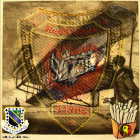
\includegraphics[width=0.1\textwidth]{avatar.png}} \hfil \parbox{0.4\textwidth}{\raggedright etcher \\ Cpt, 319th Rgt \\ \inmem{}}%

\hfill \parbox{0.3\textwidth}{\raggedright \hfill } \hfil \parbox{0.4\textwidth}%
{\centering \includegraphics[width=0.37\textwidth]{signature.png}\par}%   
\end{flushright}%

\vfil%
%\end{imini}
% \end{minipage}
%\end{onepage}%
%\import{./intro/}{pub_letter.tex}
%
\pagestyle{intro}%
%
%\chapter*{Remerciements}
%\phantomsection
%\addcontentsline{toc}{chapter}{\protect\numberline{}Remerciements}
\invisibleunnumberedchapter{Remerciements}%

\begin{imini}
Mes sincères remerciements à la \thirdwing{} pour les années passées à faire le zouave en votre excellente compagnie, et tout particulièrement aux membres du \rgt{} \inmem{}, qui me supportent depuis que Gilles m'a appris à freiner le rotor et à ouvrir la portière.

%\vfil
Les ressources graphiques utilisées dans ce document proviennent soit d'une publication Joint disponible publiquement sur Internet, et sont alors référencées comme telles, ou sont libre de droits.

Un grand merci à la \onethreetwo{}, qui m'a initié au Close Air Support, et qui invite régulièrement la \thirdwing{} à des événements bluffants de réalisme.

%\vfil

Un remerciement tout particulier à Neck, du \onethreetwo{}, qui investit une quantité de temps et d'énergie énorme pour transmettre le virus du Close Air Support aux autres passionnés.

%\vfil

Merci à la \onethreetwo{} également pour m'avoir autorisé à inclure leurs GRGs dans ce document à titre d'exemple.

%\vfil

Enfin, un clin d'oeil au suédois Renik, en charge du 696th vSquadron, sister-squadron du \rgt{} à la \onethreetwo{}.
\end{imini}

\vfil%
%
%\thispagestyle{default}

% \section*{Préface}
% \phantomsection
% \addcontentsline{toc}{section}{\protect\numberline{}Préface}
\invisibleunnumberedchapter{Résumé}%

%\setlength{\parindent}{10em}
\begin{imini}
\subsection*{Cadre}

\vfil

Ce document décrit les procédures \acrfull{cas} Joint en vigueur telles que décrites dans le \jp{}.

\vfill

\subsection*{Trivia}

\vfil

De par sa nature inter-armes, le Close Air Support (CAS) nécessite un ensemble de procédures reconnues et utilisées par toutes les parties; c'est pourquoi les procédures Joint décrites dans le \jp{} sont utilisées.

\vfil

Le \jp{} est un publication Joint qui établit le cadre et les procédures pour la conduite du Close Air Support dans une coalition inter-armes ou internationale. Ce document est utilisé, entre autres, par les différentes composantes de l'armée américaine et par l'Organisation du Traité Atlantique Nord (OTAN).

\vfil

Les procédures du \jp{} sont implémentées de manière libérale; certaines parties ou spécificités sont omises, soit parce qu'elles ne s'appliquent pas à notre niveau, soit parce que la valeur tactique ou immersive ajoutée ne contrebalance pas suffisamment la complexité intrinsèque à leur mise en place.

\vfil

Il est entendu que les procédures implémentées sont celles qui s'appliquent tout particulièrement aux appareils à voilure tournante, et que les procédures propres aux appareils à voilure fixe sont implicitement omises ou survolées brièvement.

\vfil

\textbf{Aucune modification n'a été apportée aux procédures décrites dans le \jp{}, et toute interprétation erronée serait involontaire.}
%\setlength{\parindent}{\defaultparindent}
\end{imini}%
%\import{./intro/}{preface.tex}
%
%\thispagestyle{default}

% \section*{Journal des changements}
% \phantomsection
% \addcontentsline{toc}{section}{\protect\numberline{}Journal des changements}
\invisibleunnumberedchapter{Changements}%

\begin{table}[h]

    \centering

    %\begin{tabular}{p{3cm}p{3cm}p{7cm}}
    \begin{tabularx}{\textwidth}{ @{} p{4cm} p{3cm} X @{} }

        \textbf{Date} & \textbf{Version} & \textbf{Changements}\\ \toprule

    	\today{} & DRAFT 1 & Première ébauche soumise à l'EM pour ratification\\ 
%    	\midrule
%    	test & test &%
%    	{\begin{tabularx}{\linewidth}{ @{} X @{} }
%    	caribou \\ meuh \\ tchoutchou
%    	\end{tabularx}}\\
    	
    	\bottomrule
    	

    \end{tabularx}

    \caption[Changements]{Journal des changements}

    \label{record-of-changes}

\end{table} %
%\import{./intro/}{changelog.tex}
%
%\thispagestyle{intro}

% \section*{Conventions}
% \phantomsection
% \addcontentsline{toc}{section}{\protect\numberline{}Conventions}
\invisibleunnumberedchapter{Conventions}%

\e
    \item Organisation du document:

    {\Large Chapitre} {\large Section} Sous-section {\small Sous-sous-section}

    \item Organisation des paragraphes:

    {\Large a} . {\large 1} . (a) . {\small (1)}
    
    \item Lien interne en \textcolor{black!60}{gris}:
    
    \fullref{preparation}
    
    \item Lien externe en \textcolor{blue!60}{bleu}:
    
    \thirdwing    

    \item Exemple tiré du \jp{}:

    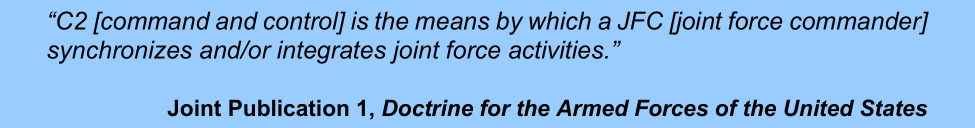
\includegraphics[width=0.7\paperwidth]{jptextex.png}

    \item Image tirée du \jp{}:

    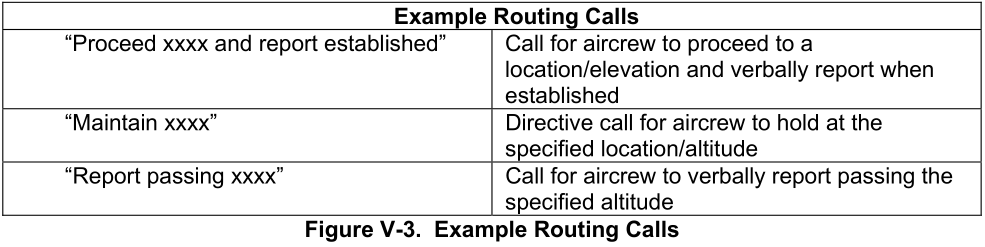
\includegraphics[width=0.7\paperwidth]{routing.png}

    \item Communication radio:
    \begin{lstlisting}
        Sochi sol, REDWOLF, pour la mise en route
        REWOLF, Sochi sol, QNH 0758, vent calme, mise en route approuv"é"e, rappelez pr"ê"t "à" rouler
    \end{lstlisting}

    \item \textbf{Emphase forte.}

    \item \emph{Emphase légère.}

    \item \important{Information importante.}
    
    %\item \useful{Information utile.}
    
    \item \remark{Remarque ou ensemble cohérent.}

    \item \note{Contenu, suggestion ou opinion qui n'est pas extrait du \jp{}.}

\ed %
%\import{./intro/}{conventions.tex}
%
\invisibleunnumberedchapter{Bibliographie}%
\nocite{*}
\printbibliography[heading=none, title=Bibliographie]%
%
\pagenumbering{arabic}%
%
\microtypesetup{protrusion=false}

\makeatletter
\renewcommand\tableofcontents{%
    \@starttoc{toc}%
}
\makeatother

\invisibleunnumberedchapter{Table des matières}%

\tableofcontents

\microtypesetup{protrusion=true}%
%
\pagestyle{default}%
%
%\chapter{Introduction}
%
%\begin{center}
%	\makebox[\textwidth]{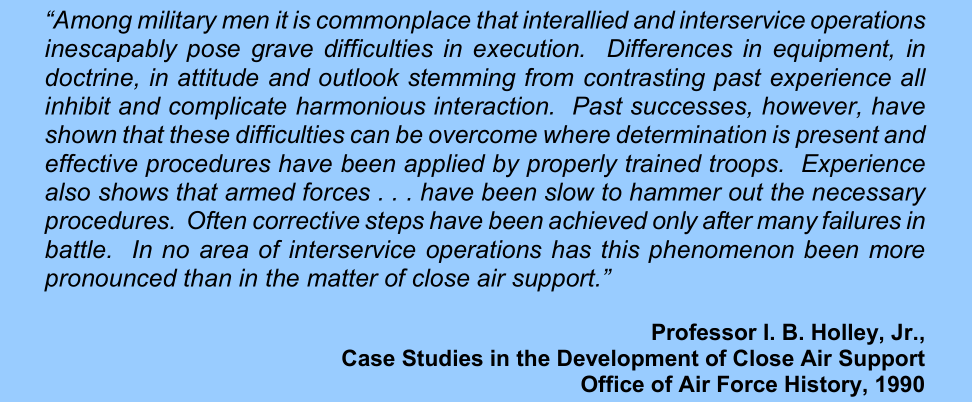
\includegraphics[width=\paperwidth]{quote1.png}}
%\end{center}

\newchapter{Introduction}{quote1}{blueonblue}%
\section{Introduction - Organisation et fondamentaux}

%
\section{Aperçu}

\begin{e1}
	\itemt{Le \acrfull{cas} est une action aérienne effectuée par les \glsfullpl{fw} et des \glsfullpl{rw} contre des cibles hostiles qui se trouvent à proximité de forces amies et qui nécessite une intégration minutieuse des missions aériennes avec le feu et le mouvement des forces amies.}{
		Le \gls{cas} demande une planification en détail, de la coordination et de l'entraînement.
		
		Le \gls{gc} soutenu par le \gls{cas} établit les priorités, les effets et le timing du \gls{cas} dans les limites de sa zone de contrôle. Le \gls{cas} donne la capacité au \gls{gc} d'employer la force aérienne pour détruire, empêcher ou neutraliser les forces ennemies et permet en conséquence le mouvement, la manoeuvre et le contrôle de territoire, de population et de zones maritimes.
		
		Le \gls{cas} est planifié et exécuté de manière à soutenir les unités au sol tactiques. Il est étroitement intégré au niveau tactique. L'allocation des appareils qui effectuent le \gls{cas} se fait au niveau opérationnel (stratégique). La planification du \gls{cas} vie à fournir un appui-feu précis et rapide aux forces amies au contact avec l'ennemi.
		
		Chaque service s'organise, s'entraîne et s'équipe pour employer le \gls{cas} selon son rôle dans la coalition. Un grand nombre d'appareils différents sont capables d'effecteur le \gls{cas}. Le \gls{jfc} et son staff ont la responsabilité d'intégrer ces capacités \gls{cas} dans leur \gls{conops}.}
	
	\itemt{Le \gls{cas} est planifié et exécuté pour appuyer les unités amies au sol.}{
		Le \gls{cas} est étroitement intégré au niveau du contrôle tactique des forces amies supportées. Alors que l'affectation des ressources aériennes disponibles se fait au niveau stratégique opérationnel, le processus de planification du \gls{cas} se fait au niveau stratégique local, pour fournir aux unités amies au contact de l'ennemi un appui-feu précis et rapide.
	}
	
	\itemt{Le \gls{cas} peut être effectué partout ou les forces amies se trouvent au contact de l'ennemi.}{
		Le mot ``rapproché'' (``Close'') n'implique pas une distance spécifique, mais plutôt un contexte. \emph{Le facteur déterminant} est la nécessité d'intégrer en détail le \gls{cas} du fait de la proximité des troupes amies. Parfois, le \gls{cas} peut être le meilleur moyen d'exploiter une opportunité tactique en défense ou en attaque. Le \gls{cas} fournit un appui-feu capable de détruire, perturber, interdire, empêcher, harceler, neutraliser ou retarder l'ennemi.
	}
	\itemt{Chaque organisation s'entraîne et emploie le \gls{cas} en tant que partie d'une coalition.}{
		Le \gls{jfc} est responsable d'intégrer ces organisations au \gls{conops} en fonctions de leurs capacités.
	}
	\itemt{Le \gls{tac} est l'autorité responsable de manœuvrer les appareils de soutien aérien et d'autoriser l'attaque finale.}{
		Un \gls{jtac} ou un \gls{faca} certifié sera reconnu comme capable et autorisé à effectuer le \gls{tac}.
		
		\fullref{controltypessection} pour un description plus détaillée des types de contrôle.
		
		Il y a trois types de contrôle (type 1, 2 et 3):
	}	
	\begin{e2}
		\itemt{\glsfull{typeone}}{
			Le \gls{typeone} est utilisé lorsque le \gls{jtac}/\gls{faca} a besoin de contrôler de chaque attaque individuellement ainsi que d'avoir en permanence en visuel l'appareil qui attaque ainsi que sa cible.
		}
		
		\itemt{\glsfull{typetwo}}{
			Le \gls{typetwo} est utilisé lorsque le \gls{jtac}/\gls{faca} a besoin de contrôler chaque attaque mais qu'il ne peut pas voir l'appareil au moment du largage ou qu'il ne peut pas voir la cible.
		}
		
		\itemt{\glsfull{typethree}}{
			Le \gls{typethree} est utilisé lorsque le \gls{jtac}/\gls{faca} a besoin de contrôler chaque engagement, avec ses restrictions, mais qu'on engagement peut être composé de plusieurs attaques.
		}
		
	\end{e2}
	
	\itemt{\glsfull{tac}}{Le \glsfull{tac} est l'autorité qui contrôle la manoeuvre des appareils de \gls{cas} et qui autorise le tir de munitions.}
	
	\itemt{\glsfull{tgo}}{
		La guidance terminale diffère \gls{tac}. Les \glspl{tgo} sont les actions qui fournissent des informations additionnelles quant à la position de la cible, par des moyens électroniques, mécaniques, visuels ou vocaux.
		
		A moins qu'il aie la qualification de \glsfull{jtac}, le personnel qui effectue la \gls{tgo} n'a pas l'autorité pour contrôler la manoeuvre des appareils de \gls{cas}, ou pour autoriser le tir de munitions.
	}
		
\end{e1}
	
%
\section{Usage du CAS}

Le \glsfull{cas} est utilisé pour attaquer l'ennemi dans un dans le cadre du \gls{conops}, dans un grand nombre d'environnements, de jour comme de nuit, et comme appui-feu. La vitesse, la portée et la manoeuvrabilité des unités aériennes leur permettent d'attaquer des cibles hors de portée des unités au sol ou navales conventionnelles.

Les \glspl{gc} sont l'autorité ultime pour l'usage de la force dans leur zone de contrôle, et décident des cibles prioritaires, des effets qu'ils souhaitent, et du timing du \gls{cas}.

\begin{e1}
	
	\itemt{Utilité sur le champ de bataille}{
		Le \gls{cas} donne aux \glspl{gc} un appui-feu flexible et réactif.
		
		En utilisant le \gls{cas}, les \glspl{gc} peuvent mieux tirer parti des opportunités qui se présentent sur le champ de bataille, en concentrant la puissance de feu pour pousser un avantage tactique, ou pour réduire les risques tactiques et opérationnels. Le mobilité de la vitesse des forces aériennes donnent aux \glspl{gc} un moyen de frapper l'ennemi rapidement et de manière inattendue.
	}
	
	\item Critères pour l'usage du \gls{cas}:
	
	\begin{e2}
		\item Mission et \gls{conops}.
		\item Disposition, force et composition de l'ennemi.
		\item Capacités et limitations des appareils engagés dans le \gls{cas}.
		\item Emplacement et équipement des \gls{jtac}.
		\item \glspl{roe}.
		\item \gls{spins}.
		\item Défenses anti-aériennes ennemies et capacités alliées à les contrer.
		\item Disposition des forces amies
		\item Allocation des sorties \gls{cas}.
		\item Emplacement des civils et estimation des dommages collatéraux potentiels.	
	\end{e2}
	
	\item Les cibles du \gls{cas} sont sélectionnées par le \gls{jtac}, en commençant analyser les intentions du \gls{gc}, puis en fonction du terrain, de la météo, de la mission, des défenses ennemies, de l'armement disponible, du temps de réponse, des capacités ou limitations propres aux appareils de \gls{cas} présents, etc. D'autres considérations sont également à prendre en compte, comme la géométrie d'attaque, la proximité des forces amies, les dommages collatéraux potentiels, la capacité des senseurs, et l'appui-feu supplémentaire disponible.
	
	Les pilotes gardent la responsabilité d'émettre des recommandations quant à l'usage optimal de l'armement et l'emploi de tactiques spécifiques, pendant que le \ja{} se concentrent sur l'obtention de l'effet désiré (\fullref{chap3} pour les tactiques d'emploi des appareils).
	
	Les \glspl{gc}, \glspl{jtac}, \glspl{faca} et les pilotes peuvent utiliser les \glspl{bda} pour déterminer les objectifs ont été remplis, ou si une nouvelle attaque est nécessaire.
\end{e1}
	
%
\section{Intégration du CAS}

Lors des opération conjointes, l'intégration du \gls{cas} commence au niveau opérationnel. S'il est établi, le \gls{jfacc} fournit ses recommandations au \gls{jfc}. Chaque composante informe le \gls{jfc} de ses besoins et limitations. Le \gls{jfc} implémente le cadre dans lequel les opérations d'interdiction (\gls{cas}, \gls{ai}, etc.) s'intégreront dans l'\gls{opord}, l'\gls{aod}, l'\gls{ato}, l'\gls{aco} et les \gls{spins}.

Le \gls{jfacc} donne ses recommandation quant à l'allocation des appareils au \gls{jfc} après avoir consulté ses composantes subordonnées.

Une fois que le\gls{jfc} a décidé de l'allocation des appareils aux différentes missions (\gls{cas}, \gls{das}, \ldots{}), le \gls{jfacc} taske les appareils de manière à remplir les différentes \glspl{req} reçues.

Le \gls{conops} du \gls{jfc} fournit le cadre pour intégrer les opérations Joint (\gls{cas}, \gls{das}, \ldots{}) dans l'\gls{opord}., les \glspl{aod}, l'\gls{ato}, l'\gls{aco} et les \gls{spins}.

%
\section{Emploi des voilures fixes et des voilures tournantes en opérations de CAS}

La structure organisationnelle, la mission principale et les capacités des appareils capables d'effectuer le \gls{cas} déterminent leur emploi. Bien que les \glspl{fw} et les \glspl{rw} puissent tous deux effectuer le \gls{cas}, leur emploi diffère.

\begin{e1}
	
	\itemt{Considérations d'ordre général}{
		L'emploi des appareils se fait en \emph{sorties}. Une sortie équivaut à \emph{un vol} pour \emph{un appareil}. Généralement, les appareils \gls{cas} volent par groupe de deux ou quatre, c-à-d deux à quatre sorties.
	}
	
	\itemt{Considérations pour les \glspl{fw}}{
		De par leurs vitesse et portée, les \glspl{fw} donnent au \gls{jfc} la possibilité de délivrer une importante puissance de feu à l'endroit et au moment souhaité. De plus, les \glspl{fw} peuvent embarquer un arsenal varié d'armement et de senseurs, leur permettant d'accomplir leur mission par tous les temps et dans des conditions météo difficiles..
	}
	
	\itemt{Considérations pour les \glspl{rw}}{
		Les \glspl{rw} permettent de manoeuvrer et de repositionner rapidement la puissance de feu en fonction de l'évolution de la situation. Ils ont un excellent temps de réponse et peuvent rester longtemps sur zone, évoluer à très faible altitude, et effectuer du \gls{cas} sur tous les types de terrain. Ils offrent également des capacités d'infiltration et d'extraction du personnel.
	}

\end{e1}

%
\section{Utilisation de drones pour le CAS}

\emptypage{}%
\section{Efficacité du CAS}

\begin{e1}
	\item 
	Pour que le \gls{cas} soit efficace, il faut:
	\begin{e2}
		\itemt{Du personnel correctement entraîné}{
			L'entraînement au \gls{cas} doit intégrer toutes les manoeuvres et procédures nécessaires à l'exécution du \gls{cas}. Cet entraînement doit être tenu à jour.
		}
		
		
		\itemt{Un planning et une intégration réfléchie}{
			Un \gls{cas} efficace s'appuie sur une planification en profondeur. La capacité à fournir la puissance de feu nécessaire au bon endroit est possible de par l'intégration avec les forces au sol. De point de vue du planificateur, le \gls{cas} pré-planifié sera toujours préféré.
		}
		
		\itemt{Un \gls{cc} efficace}{
			Le \gls{cas} nécessite une structure \gls{cc} flexible et intégrée au reste du dispositif pour trier les demandes, assigner les priorités et les tâches, repositionner les éléments, fournir les alertes de menaces, et augmenter les capacité de \gls{cid}.
			
			Pour ce faire, le \gls{cc} a besoin d'une communication fiable entre les pilotes, les agences de contrôle, les \glspl{jtac}, les forces au sol, et les \glspl{gc}.
			
			De par l'utilisation mesurée des \glspl{acm} et des \glspl{fscm}, les \glspl{gc} peuvent faciliter l'emploi du feu dans leur zone.
			
			Cfr. \citetitle{jp352} pour plus d'explications concernant les \glspl{acm}.
			
			Cfr. \citetitle{jp309} pour plus d'explications concernant les \glspl{fscm}.
			
			Cfr. \citetitle{jp330} pour plus d'explications concernant \gls{cc} en opération Joint.
		}
		
		\item La supériorité aérienne (tout particulièrement le \gls{sead}).
		
		\itemt{Marquage des cibles}{
			Fournir des marques appropriées et au bon moment permet d'améliorer grandement l'efficacité du \gls{cas}. Le marquage augmente la \gls{sa}, permet d'identifier une cible unique parmi d'autres, diminue le risque de tir fratricide et de dommage collatéral, et facilite le \gls{tac}.
			
			Si un \gls{gc} prévoit tomber à court de marques, il devra le spécifier lors de la phase de planification.
			
			\fullref{chap3} pour plus d'informations à propos de la marque.
		}
		
		\item Une reconnaissance et une connaissance des cibles
		
		\itemt{Des procédures flexibles et éprouvées}{
			Un appui-feu réactif permet au \gls{gc} de répondre aux changements rapides du champ de bataille. Comme le champ de bataille moderne est extrêmement dynamique, les procédures \gls{cas} doivent permettre de changer de cible, d'arme ou de tactique très rapidement. Le demandeur est souvent le plus à même de déterminer les besoins en termes d'appui-feu, et comme tout appui-feu, le \gls{cas} se doit d'être réactif pour être efficace.
			
			Certaines techniques peuvent être utilisées pour améliorer le temps de réponse du \gls{cas}:
		}
		\begin{e3}
			\item Placement des unités de \gls{cas} proche de leur zone d'opération. Placement des points d'attente de d'orbite de manière optimiser le temps de réaction.
			\item Délégation des autorisations de tir aux unités subordonnées.
			\item Ré-assignation des appareils en fonction des situations émergentes.
			\item Révision de l'\gls{ato} en fonction des situations émergents.
			\item Redirection des appareils \gls{cas} en réponse aux menaces.
			\item Délégation des autorité au plus bas niveau tactique possible.
			\item Placement des \gls{jtac} avec les unités au sol de manière à faciliter les communications et la coordination avec les appareils de \gls{cas}.			
		\end{e3}
		
		\itemt{De l'armement approprié}{
			Le \gls{gc} et le \gls{jtac} doivent connaître l'effet de l'armement employé, de manière à pouvoir évaluer les possibilités de dommages collatéraux, et l'impact sur le poursuite de la mission.
			\item Des conditions environnementales.
			
			Des conditions favorables améliorent l'efficacité des unités de \gls{cas} quelles que soient les capacités de l'appareil ou de l'armement. \textbf{Avant d'envisager une mission de \gls{cas}, des conditions météo minimales doivent être définies}. Certaines conditions peuvent n'influencer que certaines plateformes; par exemple, un plafond très bas peut rendre certains \glspl{fw} inutiles, sans impacter les \glspl{rw}. Inversement, les \glspl{fw} pourront opérer lors d'une tempête de sable qui clouerait les \glspl{rw} au sol. Les conditions météo influencent également fortement le marquage de la cible.
		}
		
		\efig{caswwi}{Le CAS pendant la première guerre mondiale.}
	\end{e2}
\end{e1}

%
\section{Responsabilités}

\begin{e1}
	\itemt{\glsfull{jfc}}{
		Le \gls{jfc} établit le cadre et les priorités pour le \gls{cas} dans le \gls{conops}.
	}
	
	\itemt{\glsfull{jfacc}}{
		Le \gls{jfacc} reçoit du \gls{jfc} l'autorité pour créer des missions et des tâches pour les unités aériennes sous son contrôle.
	}
	\itemt{Commandant d'escadrille/d'escadron}{
		Le commandant d'escadrille/d'escadron s'assure que ses unités subordonnées sont capables d'exécuter des missions de \gls{cas}.
	}

\end{e1}
%
\section{Minimiser le tir fratricide}

\begin{e1}
	\itemt{Général}{Le tir fratricide est parfois le résultat tragique de la guerre.}
	
	\item{Causes}{
		Bien que parfois le résultat d'armement défectueux, le tir fratricide est souvent le résultat de la confusion qui règne sur le champ de bataille.
		
		\note {Kakane, celle-là est pour toi !}
		
		Les causes peuvent être, entre autres:
		\begin{e2}
			\item Mauvaise identification de la cible.
			\item Position ou description de la cible erronée.
			\item Mauvaise transmission de la position ou de la description de la cible.
			\item Perte de \gls{sa} par le pilote ou le \gls{jtac}.
		\end{e2}
		
		Pour réduire le risque de tir fratricide, on peut employer:
		\begin{e2}
			\item Planification de mission détaillée.
			\item Procédures standardisées.
			\item Entraînements et répétitions réalistes.
			\item Utilisation d'appareils de marquages ou de tracking des unités alliées.
			\item Staff efficace.
			\item \gls{faca}.
			\item Autorisations de tir réfléchies.
		\end{e2}
	}
	
	\itemt{Responsabilités}{
		Tout le personnel impliqué dans le \gls{cas} est responsable de la sécurité lors du planning et de l'exécution. Chaque participant doit tout entreprendre pour identifier les unités alliées, les forces ennemies et les civils avant de prendre pour cible, d'engager, ou d'autoriser le tir.
		
		Le \glsfull{cid} est le processus par lequel on obtient une classification des objets détectés dans un environnement de combat suffisamment satisfaisante que pour autoriser un engagement.
		
		En fonction de la situation, cette classification peut être limitée à ami, ennemi, neutre ou non-combattant, ou inclure des informations supplémentaires comme la classe, le type, la nationalité ou la configuration.
		
		La \gls{cid}, en corrélation avec les \glspl{roe}, permettent de décider d'autoriser ou d'empêcher l'utilisation d'armement létal.
	}
	\itemt{Entraînement}{La coalition, ses composantes, et les unités doivent effectuer un entraînement conjoint régulier qui simule des opérations réelles de manière à développer les capacités nécessaires au bon déroulement du \gls{cas}.
	}
	
\end{e1}

%
\section{Minimiser les victimes civiles}
\begin{e1}
	\item Les lois de la guerre obligent tous les commandants à prendre toutes les précautions nécessaires pour minimiser les victimes civiles et les dégâts collatéraux.
\end{e1}%
%
%\chapter{Command and Control}
%
%\begin{center}
%    \makebox[\textwidth]{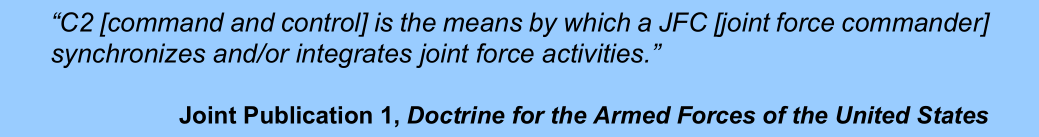
\includegraphics[width=\paperwidth]{quote2.png}}
%\end{center}

\newchapter{Command and Control}{quote2}{003}%
\section{Introduction}

\begin{e1}
	\item Le \gls{cas} requiert une structure \gls{cc} intégrée, flexible, et qui réagit rapidement.
	
	\item Le \gls{jfc} exerce son \gls{opcon} via les commandants des différentes composantes, le \gls{jfacc} pour le \gls{cas} (généralement).
	
	Pour ce faire, uns structure de communication fiable et sécurisée est nécessaire.
	
	La \smallref{jfcopcon} illustre, à titre d'exemple, l'implémentation complète de la structure \gls{opcon} du \gls{jfc}.
	
	\note{
		Implémentation DCS: \\
		\begin{e2}
			\item Les parties représentées se limiteront généralement au \gls{jfc}, \gls{jfacc}, et \glspl{gc} (équivalents au ``CP'' sur l'image).
			\item Ces nombreux rôles seront généralement soit totalement ignorés, soit remplis par la même personne. Dans la plupart des cas, le créateur de mission fera office de \gls{jfc}, \gls{jfacc} et \gls{gc}.
		\end{e2}
	}
\end{e1}

\efig{jfcopcon}{Structure OPCON du JFC.}

\begin{figure}[H]
	\import{./tikz/}{2011simplopcon}
	
	\caption{Structure OPCON simplifiée.}
	\label{fig:simplopcon} 
\end{figure}%
\section{Le CAS en opération mixte}

\begin{e1}
	\item Il n'y a pas de structure \gls{cc} pré-établie unique pour les opérations de \gls{cc}.
\end{e1}%
\section{C2 Air Force}

\emptypage{}%
\section{C2 armée de terre}

\emptypage{}%
\section{Intégration armée de terre et Air Force pour une opération au sol}

\emptypage{}%
\section{C2 Naval}

\emptypage{}%
\section{C2 Corps des Marines}

\emptypage{}%
\section{C2 Naval \& Corps des Marines en opération amphibie}

\emptypage{}%
\section{C2 Opérations Spéciales (SPECOPS)}

\emptypage{}%
\section{Systèmes de communications}

\begin{e1}
	\itemt{Contrôle et flexibilité}{
		Les missions \gls{cas} demandent un contrôle rapproché, rendu possible par des communications efficaces. Les communications doivent être flexibles et rapides pour s'assurer que le lien entre les unités au sol et les appareils qui les soutiennent est maintenu.
	}
	
	\itemt{Sécurisation des communications}{
		Lorsque c'est possible, les communications seront sécurisées, soit en cryptant les données, soit en utilisant des sauts de fréquence (système HAVEQUICK).
		
		Cependant, il ne faut pas laisser la sécurisation des communications entraver l'exécution rapide de la mission de \gls{cas}, tout spécialement dans les situations d'urgence.
	}
	
	\itemt{Contre-mesures}{
		Le brouillage, la surveillance ou l'usurpation d'identité par l'ennemi sur les réseaux radios alliés peuvent empêcher la bonne réalisation du \gls{cas}.
		
		\begin{e2}
			\itemt{Jamming}{
				Le jamming consiste à brouiller une fréquence radio pour y dégrader et ainsi empêcher les communications.
				
				Pour se prémunir contre le jamming, le \gls{complan} devra prévoir des fréquences de travail alternatives, que les différentes parties auront reçu comme consigne d'utiliser en cas de brouillage.
			}
			
			\itemt{Spoofing}{
				Le spoofing consiste à usurper l'identité d'une autre station sur le réseau et à se faire passer pour cette station lors des communications.
				
				Cela permet notamment de donner des informations ou des ordres aux unités adverses.
				
				Pour se prémunir contre le spoofing, on utilisera l'authentification, et la vigilance (procédure \gls{ginger}).
			}
			
			\itemt{Monitoring}{
				Le monitoring consiste à écouter une fréquence ennemie, et à y collecter des informations quant aux positions, mouvements, intentions, etc. de l'ennemi.
				
				Il n'y a aucun moyen de savoir si un ennemi écoute la fréquence de travail, c'est pourquoi existent les procédures \gls{comsec}.
				
				Dans le cas ou une station sur un réseau diffuse en clair des informations importantes, on utilisera la procédure \gls{bead}.
			}
			
		\end{e2}
		
		Il n'existe aucune technique permettent de se protéger contre toutes les formes d'attaque sur un réseau radio, et l'environnement tactique, les moyens disponibles et la mission elle-même détermineront les méthodes \gls{comsec} à employer.
		
		\todo[inline]{ajouter un lien vers la procédure AET100}
		
		\note{Dans DCS, nous avons à notre disposition deux méthodes principales pour protéger les communications: \glsfull{ur} et l'authentification. \\

			\gls{ur} permet de crypter les communications (A-10C seulement).\\
			
			L'authentification permet, lors de l'établissement des communications entre deux parties, de s'assurer que l'unité contactée est bien un allié.}

	}
	
	\itemt{Nécessités pour les communications Joint}{}
	
	\begin{e2}
		
		\item Les participants au \gls{cas} utiliseront le réseau de l'unité demandeuse
		
		\item Tous les participants au \gls{cas} doivent connaître les signaux et codes appropriés, et avoir toutes les données nécessaires.
		
		Le \gls{jfacc} (ou le \gls{jfc} si le \gls{jfacc} n'est pas implémenté) est responsable de la diffusion de ces informations dans les \gls{spins} ou dans l'\gls{ato}.
		
		\item Plus spécifiquement, les appareils \gls{cas} et leurs pilotes auront besoin des call-signs et fréquences de travail des différentes agences de contrôle de l'espace aérien, des forces au sol et du \gls{jtac} avec lesquels ils devront travailler.
	\end{e2}
	
	\itemt{Réseaux radios}{
		Un certain nombre de réseaux radios sont systématiquement utilisés pour le \gls{cas}, parmi lesquels (liste simplifiée pour DCS):
	}
	
	\begin{e2}
		\itemt{Réseau \gls{cc}}{Interface entre les unités \gls{tacs}}
		\itemt{Réseau \gls{tad}}{
			Ce réseau est utilisé par tous les participants au \gls{cas}, \glspl{tacp}/\glspl{jtac} et appareils de \gls{cas}, et doit être réservé au \gls{tac}. Le \gls{asoc} est autorisé à y faire intrusion pour le passage d'information d'extrême urgence.
		}
		\itemt{Réseau \gls{infltrep}}{
			Ce réseau est utilisé pour la transmission est \glspl{infltrep} aux éléments de \gls{tacs}. Ces rapports sont normalement envoyés à l'\gls{awacs}. Lorsque c'est possible, ce réseau est écouté par l'\gls{asoc} et l'\gls{aoc}.
		}
		\itemt{Réseau de garde}{
			Ce réseau est un réseau d'urgence pour les appareils en détresse. Il sert également aux agences de contrôle pour la transmission pour avertir les appareils en vol d'une situation dangereuse ou de dangers pour le vol. Si possible, tous les appareils doivent continuellement ce réseau.
		}
		\itemt{Réseau de l'escadron}{Chaque escadron dispose de son réseau propre.}
		\itemt{Réseau \gls{tacp} administratif}{Réseau utilisé pour la transmission d'informations entre l'\gls{asoc} et les \glspl{tacp}}.
		\itemt{\glsfull{irc}}{Réseau sécurisé permettant l'échange d'informations entre les services de renseignement, les appareils équipés, l'\gls{asoc}, et les \glspl{tacp} et \glspl{jtac} équipés.
			\note{Le réseau \gls{irc} peut effectivement être simulé dans DCS par le chat TeamSpeak textuel.}
			}
	\end{e2}
\end{e1}%
\section{Renseignements}

\emptypage{}%
%
\chapter{Planification et demande}

\begin{center}
	\makebox[\textwidth]{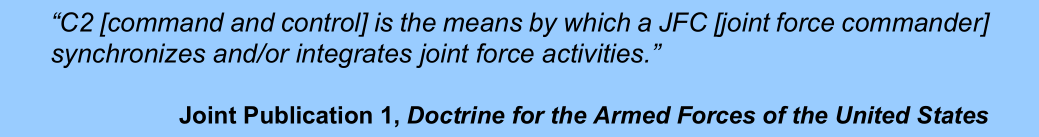
\includegraphics[width=\paperwidth]{quote3.png}}
\end{center}

\newpage




%


\section{Introduction}

Ce chapitre décrit le processus de prise de décision \gls{cas}, décrit les responsabilités du staff, établit les bases de ce qu'il y a lieu de prendre en compte lors de la planification, et établit les procédures de \glspl{req}.

La phase de planification commence lorsque l'unité reçoit l'ordre du Haut Commandement.

Bien que chapitre se concentre principalement sur les tâches à effectuer lors d'opération complexes, les même tâches peuvent s'appliquer aux opérations d'exfiltration, de \gls{csar}, qui pourraient avoir une structure de commandement différente.


\begin{e1}
	\item Il existe deux types de \gls{cas} distincts:
	\begin{e2}
		\item Le \gls{cas} planifié
		\item Le \gls{cas} immédiat
	\end{e2}
\end{e1}
\todo{p68}

\begin{e1}
	\item Le \gls{req} est effectué par l'unité qui demande un soutien aérien. On distingue deux principaux types de demandes:
	\begin{e2}
		\item Le \gls{cas} planifié à l'avance (``pre-planned \gls{cas}'', ou simplement ``\gls{cas}'')
		\item Le \gls{cas} ``à la demande'' (``on-call cas''), qui regroupe deux possiblités:
		\begin{e3}
			\item Le \gls{xcas}, où l'appareil en attente de tasking se trouve déjà dans les airs
			\item Le \gls{gcas}, où l'appareil en attente de tasking se trouve encore au sol
		\end{e3}
	\end{e2}
	\item Un \gls{req} réel se compose d'un grand nombre d'informations, utiles à la planification de la mission et à la répartition des effectifs disponibles.
	\item
	Souvent, pour DCS, l'équivalent du \gls{req} sera contenu dans le briefing de la mission (zone d'opération, menace, composition et force de unités ennemies, timing, emport, unités amies, \gls{jtac}, plan de fréquences, etc…).
	\item Toute référence ultérieure au \gls{req} fera donc implicitement référence au briefing de mission.
	\item Les considération à prendre en compte lors de l'établissement d'une \gls{req} sont propres au rôle de \gls{gc}/\gls{jfc} et ne seront pas traitées dans ce document.
	\item Le \gls{cas} planifié est un \gls{cas} effectué après une \gls{req} spécifique, concernant une zone connue, pour atteindre un objectif déterminé.
	\item Dans le cas d'un \gls{cas} planifié, un grand nombre de paramètres sont connus avant le décollage, ce qui permet une meilleure préparation.
\end{e1}

\subsection{Étape 1: réception de l'ordre de mission}

\begin{e1}
	\item
	En tant que participants au processus de planification, les officiers en charge (chef de patrouille, commandant d'escadron, …) devraient être à même de comprendre et analyser l'information à partir de ces différentes sources:
	\begin{e2}
		\item \gls{aob}
		\item \gls{ato}
		\item \gls{aco}
		\item \gls{spins}
		\item \gls{opord}
		\item \gls{sop}
	\end{e2}
\end{e1}
\note{Les \glspl{sop} sont propres à l'escadron, et sont normalement connues par les tous les officiers supérieurs.\par
	
	Exceptées les \glspl{sop}, tous les éléments sont normalement fournis sous une forme ou l'autre dans le briefing de mission.\par
	
	S'il devait manquer un élément, il appartient à l'officier en charge de la patrouille d'évaluer son importance et de poser les questions nécessaires à l'organisateur de la mission.\par
}

\subsection{Étape 2: analyse de la mission} 

\begin{e1}
	\item Avant de pouvoir préparer la mission, les officiers en charges devront:
	\begin{e2}
		\item Mettre à jour les différentes sources d'informations (\gls{ato}, \gls{spins}, \gls{aco}, …)
		\item Estimer les capacités des forces à leur disposition (équipement, personnel, restrictions, …)
		\item Déterminer les tâches essentielles de la mission
		\item Évaluer les conditions relatives à:
		\begin{e3}
			\item L'ennemi
			\item La météo
			\item Le terrain
		\end{e3}
		\item Avertir les unités (personnes) subordonnées
	\end{e2}
	\item Considérations clefs à prendre en compte lors de l'analyse de la mission:
	\begin{e2}
		\item \gls{conops}: Quelles sont les intentions du \gls{jfc}? Attaque ou de défense? Surprise ou délibéré? Règles d'engagement?
		\item Comment s'intègre le \gls{cas} au reste du dispositif?
		\item Quelles pourraient être les intentions de l'ennemi? Comment ces intentions sont-elles affectées par le terrain, la météo, l'heure ?
		\item Quels sont les moyens de surveillance ou de reconnaissance à notre disposition?
		\item \gls{complan} Comment vont s'organiser les communications? Est-ce que toutes les unités participantes au \gls{cas} sont intégrées au \gls{complan}  de manière fiable et redondante?
	\end{e2}
	\item Dans le cas d'une demande de \gls{cas} pré-planifié, un grand nombre d'informations supplémentaires pourront être obtenues via la demande elle-même. Par exemple:
	\begin{e2}
		\item Zone de \gls{cas}
		\item Menaces
		\item Type de cibles
		\item Localisation de la cible
		\item Localisation des forces amies
		\item Type de terrain
		\item Restrictions horaires
		\item \gls{jtac}
	\end{e2}
\end{e1}

\subsection{Étape 3: préparation de la mission}

\begin{e1}
	\item Le ``Mission planning'', ou ``préparation de la mission'', est une étape cruciale au bon déroulement de cette dernière.
	\item Cette préparation sera effectuée par le chef de patrouille, qui sera chargé de rassembler et analyser toutes les informations à sa disposition pour préparer au mieux la mission de la patrouille dont il a la charge.
	\item Lorsque c'est possible, la préparation de la mission se fait en collaboration avec les différents éléments impliqués, certainement avec le \gls{jtac} en charge de la zone attribuée à la patrouille, le \gls{tacon}, et les autres chefs de patrouilles opérant dans le même théâtre opérationnel.
	\item Le chef de patrouille veillera tout particulièrement à toujours utiliser les informations les plus récentes, et fera attention à se tenir au courant de l'évolution de la situation.
	\item Il devra également s'assurer que tous les éléments sous son contrôle ont reçu et compris ses intentions pour la mission.
	\item Checklist de préparation de mission. \fullref{ann1}
\end{e1}

\section{Le CAS immédiat}

\begin{e1}
	\item Le \gls{cas} immédiat intervient lorsque la situation sur le champ de bataille évolue de manière inattendue.
	\item L'\gls{ato} peut allouer un certain effectif pour se préparer à répondre à ces situations.
	\item Le chef de patrouille trouvera alors dans cet \gls{ato} les informations nécessaires pour préparer son vol (emport, point d'attente, etc…).
	\item
	Pendant le vol (ou au parking pour le \gls{gcas}), si l'intervention de la patrouille s'avère nécessaire, celle-ci recevra un point de contact initial, ainsi que le call-sign et la fréquence de l'agence qui s'occupera de son contrôle terminal.
\end{e1}





\newpage
\section{Mission}

Le \gls{cas} est intégré au reste du dispositif de la coalition en opérations défensives et offensives, pour détruire, neutraliser, interdire, retarder ou empêcher le mouvement de l'ennemi.
\e
	\item Le \gls{cas} peut servir pour renforcer les opérations annexes, soutenir l'effort majeur ou établir les zones de sécurité
	\ee
		\itemt{Opérations annexes}{
		Bien que ce ne soit pas vocation principale, le \gls{cas} peut être employé pour soutenir une opération loin en territoire ennemie (infiltration, exfiltration, opérations spéciales), ou pour une opération ponctuelle}
		\itemt{Opérations de combat rapproché}{
		Le plus souvent, le \gls{cas} servira à renforcer l'effort de guerre principal. Les appareils de \gls{cas} ajoutent leur force aux forces au sol pour soutenir les \glspl{gc}. La vitesse et la portée du \gls{cas} en font un élément idéal pour exploiter les avancées amies, contrer les manoeuvres adverses ou poursuivre un ennemi en fuite.}
		\itemt{Opérations de sécurité}{
		Le \gls{cas} est efficace pour empêcher la pénétration de l'ennemi. Le temps de réponse et la puissance de feu du \gls{cas} peut augmenter de beaucoup la force des unités au sol.}
	\ed
	\item Le \gls{cas} peut servir pour les opérations offensives, défensives et de stabilité
	\ee
		\itemt{Le \gls{cas} en support de l'offense}{
		\eee
			\itemt{Mouvement vers le contact}{
			Le \gls{cas} peut servir à appuyer les forces au sol qui font mouvement. Une fois le contact avec l'ennemi établi, le \gls{cas} peut les submerger et accélérer le déploiement des forces alliées. \textbf{Pendant la planification de l'intégration du \gls{cas} à l'avancée alliée, il est recommandé de déployer les appareils tout le long de l'axe de progression.}}
			\itemt{Attaque}{
			Les \gls{gc} peuvent utilser le \gls{cas} pour attaquer directement l'ennemi. Le \gls{cas} peut détruire les unités ou capacités ennemies importantes avant que l'ennemi ne puisse établir de défense. Le \gls{cas} peut également servir à renforcer la puissance de feu lors d'une attaque, ou pour isoler une force ennemie sur le champ de bataille et la forcer à prendre une position défensive.}
			\itemt{Exploitation}{
			L'exploitation est une tactique offensive utilisée après une attaque réussie, et sert à déstabiliser l'ennemi, en coupant les voies d'accès, en détruisant les forces qui font retraite, et pour frapper les cibles d'opportunité lorsque la cohésion de l'ennemi diminue.}				\itemt{Poursuite}{
			En poursuite, le \gls{gc} attaque l'efficacité de l'ennemi en fuite alors qu'il est démoralisé et que sa cohésion et sont contrôle sont faibles. Puisque l'objectif de la poursuite est la destruction de l'ennemi, le \gls{cas} peut maintenir une pression directe et constante sur l'ennemi pour empêcher qu'il ne se réorganise ou ne se reconstitue.}
		\ed}
		\item Le \gls{cas} en support des opérations défensives alliées
		\eee
			\itemt{Support de la manoeuvre}{
			Le \gls{cas} peut s'ajouter à la puissance de feu des unités au sol en tant que membre d'une force combinée}
			\itemt{Support du mouvement}{
			Le \gls{cas} peut soutenir les éléments alliés lors de leurs mouvements entre deux positions. Les \gls{gc} peuvent utiliser le \gls{cas} pour protéger le front, les flancs ou l'arrière de la formation en mouvement.}
			\itemt{Refoulement de l'ennemi}{
			Le \gls{cas} peut servir à refouler une force ennemie qui aurait franchi ou pénétré les défenses alliées}
		\ed
		\itemt{Le \gls{cas} en opération de stabilité}{
		L'emploi du \gls{cas} en opération de stabilité est foncièrement différent de l'emploi du \gls{cas} en opération de combat. Comme l'objectif d'une opération de stabilité est d'établir la sécurité civile, rétablir les services, et restaurer et protéger les infrastructures, le \gls{cas} en opération de stabilité sera généralement restreint en terme d'échelle et des \glspl{roe} strictes seront souvent d'application. L'utilisation de \glspl{pgm} sera souvent préconisé par le \gls{jfc} lors du support de \gls{gc} en environnement urbain, de manière à limiter les dommages collatéraux.
		}
	\ed
\ed
\section{Ennemi}

Lors de la planification, il faut tenir compte de la disposition des forces ennemies, leur composition, son \gls{aob}, et ses intentions probables.

\begin{e1}
	
	\item Autres considérations:
	
	\begin{e2}
		
		\item Quelles sont les capacités offensives et défensives de l'ennemi?
		
		\item Quelles sont les capacités ennemies concernant:
		
		\begin{e3}
			\item Menaces sol-air.
			\item Leurres.
			\item Camouflage.
		\end{e3}
		
		Les cibles de hautes importance seront généralement défendue par des unités anti-aériennes. L'utilisation d'armes à très longue portée et le fait de varier les \glspl{ip} augmentera les chances de survies des appareils de \gls{cas}.
		
		\item Quelles sont les capacités de l'ennemi en terme d'\gls{ew} ou de \gls{cc}?
		
	\end{e2}
	
	\item A partir de ces informations, le planificateur peut anticiper les capacités de l'ennemi à contrer la mission alliée, et l'influence potentielle qu'aura l'ennemi sur les vols alliés.
	
	Les changements susceptibles de se produire pendant le déroulement de la mission rendent les communications avec les appareils en vol très importantes, nécessitant parfois une adaptation du plan de vol, c'est pourquoi des alternatives sont prévues dès le commencement de la mission.
\end{e1}
\newpage
\section{Troupes au sol alliées}

Le planificateur doit prendre en compte les unités \gls{cc}, \gls{isr}, \gls{ew} et \gls{cas}.

\e
	\itemt{Unités \gls{cc}}{
	Un plan \gls{cc} détaillé, flexible et redondant est essentiel. Des unités \gls{cc} aéroportées peuvent faciliter le travail du \gls{cc}, mais chaque plateforme a ses capacités et limitations qui doivent être prises en compte lors du planning. Au minimum, les points suivants doivent être évalués:}
	\ee
		\itemt{Unités \gls{cc} aéroportées}{
		Est-ce que ces unités ont une importance critique pour la mission ou seulement pour une partie de celle-ci? Quel sont le rôle et la fonction de chacune? Est-ce que le nécessaire a été fait pour assurer la communication entre le \gls{cc} et les \gls{rw} volant bas?}
		\itemt{Unités \gls{cc} au sol}{
		Intégrer les unités \gls{cc} au sol revêt une importance capitale. Quel sont le rôle et la fonction de chacune? Est-ce que le nécessaire a été fait pour assurer les communications avec le \gls{cc}?.}
	\ed
	\itemt{Unités \gls{isr}}{
	Toutes les sources d'\gls{isr} sont d'excellentes (drone, \gls{elint}, scouts, \gls{faca}, rapports des appareils d'attaque, etc.) sources d'informations.}
	\itemt{Capacités et armement des appareils \gls{cas}}{
	Le planificateur choisit les combinaisons d'appareils et d'armement qui offrent la précision, la puissance et la flexibilité nécessaires pour obtenir l'effet désiré. Le \gls{gc} doit fournir suffisamment d'informations à propos de cet effet désiré, ainsi que toute restriction tactique ou limitation. Les \gls{gc} doivent savoir qu'une \gls{req} immédiate risque d'être assurée par un appareil ne disposant pas de l'armement optimal pour la mission.}
\ed
\newpage
\section{Terrain}

\begin{e1}
	\itemt{Comment le terrain affecte le \gls{cas}}{
	Le terrain peut affecter les communications et la \gls{los}. Les unités \glspl{rw} sont particulièrement concernées. Le planificateur doit compenser ces limitations en implémentant des relais, ou intégrer ces limitations à la mission. La visibilité et le plafond peuvent affecter la décision d'employer des tactiques basse, moyenne ou haute altitude, ou l'utilisation de \glspl{rw}. Ces conditions affectent également la capacité du \gls{jtac} à voir la cible. Si des véhicules ennemis se déplacent, une colonne de fumée peut révéler leur emplacement. La visibilité a un impact plus important sur les armes à longue portée (bombe lisse, roquettes) que sur les armes à courte portée (canon, bombes freinées). Un brouillard épais a plus d'impact sur les attaques à bas niveau. Une visibilité réduite et une couche nuageuse importante peuvent restreindre l'emploi de l'armement \gls{eo}. L'acquisition de la cible est généralement plus facile lorsque le soleil se trouve derrière l'appareil qui attaque.}
	\begin{e2}
		\itemt{Masquage de la cible}{
		Une cible masquée par le terrain, un immeuble ou une couverture naturelle peut être difficile à repérer. Une altitude plus élevée peut aider.}
		\itemt{Imagerie thermique}{
		Un grand nombre de variables affecte l'efficacité de l'imagerie thermique. L'état de l'équipement, l'heure de la journée et l'arrière-plan doivent être pris en compte.}
		\itemt{Contraste et luminosité}{
		Le contraste de la cible avec son arrière plan est un facteur critique lors de la recherche de cible. Une cible camouflée devant un arrière-plan de couleur similaire peut être impossible à détecter depuis une haute altitude ou une grande distance. Toutes les cibles, quelque soit le contraste, sont plus difficiles à repérer en condition de faible luminosité.}
		\itemt{Environnement montagneux}{
		Un environnement montagneux peut forcer l'ennemi à concentrer ses forces sur les routes, dans les vallées, sur des pentes plus faibles ou dans de profond défilés, là ou le \gls{cas} est très efficace. Cependant, ce type de terrain restreint également la direction d'attaque des appareils \gls{cas}. Le planificateur doit supposer que l'ennemi va concentrer ses défenses sur l'axe d'attaque le plus probable.}
		\itemt{Environnement désertique}{
		Les appareils \gls{cas} sont rendus plus vulnérables par l'absence de couverture, et la dispersion des unités au sol.}
		\begin{e3}
			\itemt{Acquisition de la cible}{
			En général, comme le contraste entre la cible et l'arrière plan est fort, la détection sera possible à plus longue portée.}
			\itemt{Emploi des armes}{
			Un environnement désertique permettra généralement l'emploi des armes à leur portée maximale.}
			\itemt{Communications}{
			En environnement désertique, les communications sont généralement possible à plus longue portée.}
			\itemt{Menaces}{
			Les menaces seront également capables d'acquérir et d'engager les appareils \gls{cas} à portée maximale.}
			\itemt{Manque de références}{
			Le désert, de par l'absence de références distinctes au sol, rend le talk-on et l'établissement d'\gls{ip} difficiles}
		\end{e3}
		\itemt{Jungle/forêt}{
		Généralement, le contact avec l'ennemi se fera à très courte portée.}
		\begin{e3}
			\itemt{Acquisition de la cible}{
			L'acquisition de la cible peut être rendue difficile, voire impossible, par la densité des arbres, pour l'appareil qui attaque comme pour le \gls{jtac}. Dans ces conditions, il appartient au \gls{gc} de marquer la cible. Un \gls{faca} en station peut également aider de par sa \gls{sa} supérieure.}
		\end{e3}
		\itemt{Environnement urbain}{
		Le \gls{cas} en environnement présente des particularités uniques, parmi lesquelles la déconfliction en espace confiné, des \glspl{roe} particulières, la difficulté d'analyser la menace, la présence de non-combattants, le risque de dégâts collatéraux et l'augmentation du risque de tir fratricide.}
		\begin{e3}
			\itemt{Menaces}{
			La ville offre d'excellent couvertures aux unités anti-aériennes. Les \glspl{sam} ou \gls{aaa} légers peuvent être employés depuis les toits. Le terrain encombré peut rendre l'acquisition des menaces difficile. Le placement des zones d'attente est rendu difficile par la dispersion des menaces dans une grande zone urbaine. Les \glspl{rw} nécessitent un secteur sécurisé de manière à pouvoir se déplacer est être moins prévisibles. Les \glspl{fw} établissent leur zone d'attente en terrain non-hostile, mais suffisamment proche de la ville que pour pouvoir assurer un support rapide.}
			\begin{e4}
				\item Infrarouge et \glspl{nvg}
				\begin{e5}
					\item Les signatures infrarouges sont affectées par la proximité des bâtiments. La température généralement plus haute en environnement urbain affectent négativement le contraste infrarouge entre la cible et l'arrière-plan.
					\item Les lumières de la ville peuvent saturer les \glspl{nvg} et les rendre inutiles.
				\end{e5}
				\itemt{\gls{cc}}{
				L'environnement urbain présente de gros problèmes de communications du fait des immeubles qui bloquent la \gls{los} et absorbent ou reflètent les signaux. L'utilisation d'un \gls{cc} aéroporté ou de relais permet d'en minimiser l'impact.}
				\itemt{Particularités propres au \gls{jtac}}{
				Les hauts bâtiments rendent l'acquisition de la cible par le pilote difficile, et peuvent nécessiter l'emploi de \gls{fah} spécifiques. Des observateurs peuvent être placés sur les toits pour améliorer la vue d'ensemble.}
				\itemt{Efficacité}{
				Un entraînement spécifique à l'environnement urbain est nécessaire pour que le \gls{jtac} y soit efficace. Historiquement, les engagements en zone urbaine se produisent dans 90\% des cas lorsque les troupes amies se trouvent à moins de 50 mètres des forces ennemies, et 80\% des blessures en zone urbaine proviennent des débris de verre dûs aux ondes de choc et aux surpression faisant suite à une explosion. Le \gls{jtac} doit porter une attention particulière à sélectionner l'armement approprié. La situation en zone urbaine change très rapidement, de bâtiment en bâtiment. Le \gls{jtac} peut utiliser les appareils de \gls{cas} ou le \gls{faca} pour engager des forces ennemies en dehors de la zone d'engagement, pour empêcher ces dernières de renforcer la ligne de front.}
				\itemt{Navigation}{
				La navigation est plus difficile en ville. Les bâtiments ne sont pas indiqués sur les cartes. Les mouvements rapides peuvent embrouiller les observateurs au sol ou en l'air concernant les positions amies et ennemies.}
				\itemt{\gls{grg}/Grille urbaine}{
				Des cartes ou des images détaillée de la zone urbaine peuvent être établies. Ces cartes ou ces images représentent la zone urbaine et peuvent contenir des bâtiments numérotés, les zones d'atterrissage pour les \glspl{rw}, des points de références, etc. C'est la responsabilité du \gls{gc} d'établir les cartes/images pour sa zone, et d'en assurer la gestion des versions ainsi que la diffusion. \textbf{Ces grilles doivent être établies en prenant en compte ce que les appareils de \gls{cas} pourront repérer le plus facilement (rivières, carrefours, bâtiments remarquables, ponts, etc.)}. Recommandations pour la création de \gls{grg}:}
				\begin{e5}
					\item L'image doit contenir une flèche pointant vers le nord, et être idéalement orientée avec le haut vers le nord
					\item Les coordonnées est et nord doivent se trouver en haut et à gauche
					\item Les bâtiments doivent être numérotés du nord-ouest au sud-est pour de grandes zones, ou dans le sens des aiguilles d'une montre à partir de l'objectif pour de plus petites zones
				\end{e5}
				\efig{urbangrid}{Grille urbaine 1}
				\efig{grg1}{Grille urbaine 2}
				\efig{grg2}{Grille urbaine 3}
				\efig{grg3}{Grille urbaine 4}
				\efig{grg4}{Grille urbaine 5}
				\efig{grg5}{Grille urbaine 6}
				\efig{grg6}{Grille urbaine 7}
				\newpage
				\itemt{\glspl{trp}}{
				Des \glspl{trp} peuvent également être utilisés. Les \glspl{trp} sont générés en numérotant les bâtiments ou les particularités urbaines dans et autour de la zone de l'objectif. Ils peuvent être labellisés TRP\#1, TRP\#2, etc. Les \glspl{trp} permettent de passer ou interpréter un appel concernant un tir ennemi.}
				\efig{trp}{Target Reference Point}
				\itemt{Choix de l'armement}{
				L'armement à utiliser en milieu urbain doit être choisi de manière à pouvoir tirer rapidement, de manière précise, et à minimiser les dommages collatéraux. Combiner les \glspl{rw} et les \glspl{rw} peut s'avérer être une tactique judicieuse: l'aptitude du \gls{fw} à acquérir et désigner une cible en zone urbaine peut être combiné avec la capacité du \gls{rw} à utilisé une \gls{pgm} de moindre puissance depuis une \gls{bp} sécurisée. Il faut adapter le type de munitions employées: un bombe à fragmentation, très efficace contre une concentration d'unité légèrement blindées en terrain ouvert, n'est pas un choix à considérer en zone urbaine.}
				\itemt{Exigences du \gls{sead}}{
				Si la menace sol-air est importante, le \gls{cas} peut être réduit jusqu'à ce qu'elle soit suffisamment réduite. Le support \gls{sead} peut être nécessaire contre les défense sol-air ennemie, à l'intérieur comme à l'extérieur de la ville. Un \gls{sead} agressif et pro-actif peut être nécessaire au commencement d'une opération.}
			\end{e4}
			\itemt{Visibilité limitée, nuit et mauvaise météo}{
		Une visibilité limitée ou une mauvaise météo alourdissent la charge de travail du pilote et demande un pilotage et une connaissance des procédures plus pointus. Les \ja{} et les pilotes doivent régulièrement s'entraîner ensembles dans ces mauvaises conditions pour espérer être efficaces. Il y a trois grandes catégories de visibilité restreinte:}
			\begin{e4}
				\itemt{Visuel}{
			Pendant la nuit, les \ja{} et les pilotes doivent travailler avec beaucoup moins de lumières, et utiliser les feux ou les illuminations artificielles pour se coordonner. Si la menace le permet, les \gls{jtac} peuvent décider d'employer les lumières des appareils ou des flares.}
				\begin{e5}
					\item Planification pour le visuel
					\begin{e6}
						\itemt{Météo et visibilité restreinte}{
						Si le temps est clair et que la lune éclaire, l'utilisation de sources de lumière supplémentaire peut ne pas être nécessaire. Le fumée, le brouillard ou les précipitations dans la zone cible peuvent réduire la visibilité et obliger les appareils à manoeuvrer plus près des menaces.}
						\itemt{Plafond bas}{
						Un plafond bas peut forcer les appareils à voler plus bas et rendre la déconflictions aux positions d'attente difficile.}
						\itemt{Terrain}{
						Connaître le terrain est indispensable pour effectuer du \gls{cas} de nuit.}
						\itemt{Sans illuminations}{
						Attaquer une cible sans illumination supplémentaire dépend de plusieurs choses:}
						\begin{e7}
							\item La nécessité d'attaquer une cible sur un point (personne, véhicule, ou endroit) ou une zone (ensemble de bâtiments, groupe de véhicules)
							\item Lumière ambiante sur la zone cible
							\item Cible illuminée ou pas
							\item Distance oblique minimale due à la menace
							\item Restrictions propres au théâtre d'opération
						\end{e7}
						\itemt{Conditions changeantes (Aube/Crépuscule)}{
						A l'aube et au crépuscule, les \ja{} et les pilotes doivent d'adapter à des conditions qui changent rapidement. Il peut être nécessaire de changer la géométrie de l'attaque pour s'adapter aux nouvelles conditions.}
						\itemt{Illumination artificielle}{
						Dans la plupart des cas, les \ja{} et les pilotes utiliseront des \glspl{nvg} ou un \gls{flir}. Les flares sont indispensables pour des opérations de nuit sans \glspl{nvg} ou \gls{flir}. \textbf{Si possible, il ne faut pas éclairer les positions amies de nuit}.}
						\important{Toute illumination artificielle de la zone de combat de nuit doit préalablement être approuvée par le \gls{jtac}.}
						\begin{e7}
							\itemt{Fusée éclairante tirée depuis le sol}{
							Ces fusées n'éclairent pas aussi fort ni aussi longtemps qu'une LUU-2 (ou équivalent)}
							\itemt{LUU-2 (ou équivalent)}{
							Ces fusées sont prévues pour illuminer une zone pendant environ 5 minutes}
							\itemt{Roquette éclairante}{
							Une roquette éclairante est prévue pour illuminer la zone pendant environ 2 minutes.}							
						\end{e7}
						\itemt{Marques}{
						Les fusées au phosphore sont régulièrement utilisées comme marque. La lumière ambiante peut se refléter dessus et les rendre visible, même de nuit.}
					\end{e6}
					\itemt{Exécution du visuel}{
					La positions des alliés, le vent et la menace détermineront la géométrie d'attaque et l'armement employé.}
				\end{e5}
				\itemt{Assistance système}{
				De nuit, l'acquisition de la cible aidée par le système embarqué est utilisé est généralement préférée.}
				\begin{e5}
					\itemt{Laser}{
					Les procédures de nuit pour la désignation laser sont identiques aux procédures de jour.}
					\itemt{\gls{eo}/\gls{ir}}{
					La couverture nuageuse, les précipitations et les conditions du champ de bataille (fumée, poussière, ou autre) peuvent dégrader les performances infrarouge ou électro-optiques.}
					\itemt{\gls{hmcs}}{
					Dans un rôle air-sol, le \gls{hmcs} est utilisé conjointement aux autres senseurs pour augmenter la réactivité et la \gls{sa} du pilote.}
				\end{e5}
				\itemt{Emploi des \glspl{nvg}}{
				Les \glspl{nvg} sont un senseur supplémentaire pour le pilote. Les \ja{} doivent être équipés de pointeurs \gls{ir} pour en exploiter le plein potentiel.
				}
				\begin{e5}
					\item Préparation d'une mission avec \glspl{nvg}
					\begin{e6}
						\itemt{Météo}{
						Un ciel couvert peut diminuer la luminosité ambiante et marquer la silhouette de l'appareil pour les forces au sol.}
						\itemt{Marques}{
						Un pointeur \gls{ir} est le complément parfait des \gls{nvg}. Cependant, une coordination supplémentaire est nécessaire pendant la corrélation pour s'assurer que le pilote a bien acquis le bon bout du pointeur.
						}
						\itemt{Roquette, artillerie}{
						La chaleur produite par l'explosion initiale de la roquette ou de l'obus au phosphore sera clairement visible aux \glspl{nvg}.}
					\end{e6}
					\item Exécution d'une mission avec \glspl{nvg}
					\begin{e6}
						\itemt{Armement embarqué}{
						En général, toute les bombes lisses créeront à l'impact un flash de lumière qui peut être utilisé comme marque. L'explosion réchauffera le sol alentour pour un temps, ce qui peut également être utilisé comme marque \gls{ir}}
						\itemt{Équipement \gls{ir} des troupes au sol}{
						En fonction des conditions, tout le faisceau sera visible, ou juste la partie autour de la cible. Le faisceau sera étroit à sa source, sur le \gls{jtac}, et diffus sur la cible. L'illumination de la cible par le \gls{jtac} doit être la plus courte possible, de manière à ne pas compromettre la position de ce dernier si l'ennemi est également équipé de \glspl{nvg}.}
						\begin{minipage}{\linewidth}
						\itemt{Équipement \gls{ir} aéroporté}{
						Ces équipements fonctionnes généralement très bien depuis une altitude moyenne. Une lumière ambiante élevée réduira leurs performances mais ne les empêchera pas de fonctionner. Ces équipements peuvent être utilisés pour augmenter la \gls{sa} du \ja{} en marquant la cible, ou en pointant sur la même cible pour corrélation.}\\ \vskip5mm
						\important{Les appareils équipés de pointeurs \gls{ir} doivent se coordonner avec le \gls{jtac} avant de pouvoir les utiliser}
						\end{minipage}
					\end{e6}
				\end{e5}
				\itemt{Marquage des unités amies}{
				Les forces au sol alliées peuvent marquer leur position par différents moyens.}
				\begin{e5}
					\item Pointeur \gls{ir}\\
					\itemt{Marqueur \gls{ir}}
					{Pas d'application dans DCS}
					\itemt{GLINT tape}
					{Pas d'application dans DCS}
				\end{e5}
			\end{e4}
			\itemt{Paramètres d'autorisations \gls{bot} avec marqueur \gls{ir} au sol}{
			Lors de l'emploi de marqueurs \gls{ir} au sol, les pilotes devront appeler "VISUEL" lors de l'acquisition de la position amie ou "TALLY" pour l'acquisition de la position ennemie, et "CONTACT SPARKLE" à chaque passe avant d'obtenir l'autorisation de tir. La brevity propre à l'utilisation de l'\gls{ir} doit être maintenue jusqu'à l'appel "CEASE SPARKLE".}
			\itemt{CAS brief}{
			Si le \gls{jtac} à l'intention d'utiliser un pointeur \gls{ir}, ce sera indiqué dans le CAS brief, ligne 7, "Type de marque", comme "IR" ou "Pointeur IR".}
		\end{e3}
	\end{e2}
\end{e1}
\section{Timing}

\begin{e1}
	\itemt{Temps disponible}{
		Le temps nécessaire à la planification de la mission doit être estimé de manière réaliste, et ce temps doit être lui-même implémenté dans la planification.}
	
	\itemt{Cycle de planification}{
		Si une opération \gls{cas} prévue n'est pas prête au moment de son exécution prévue, elle sera d'office réassignée comme \gls{req} immédiate.}
	
	\itemt{Synchronisation}{
		Pas d'application dans DCS.
	}
	\note{
		Lors d'opération sous DCS, on distingue trois façon de donner un temps:
		\begin{e2}
			\itemt{Heure réelle (temps \gls{irl})}{
				Il s'agit de l'heure réelle, comme indiquée à nos montres.
				
				Cette heure est ajustée à la saison (heure d'été, heure d'hiver) et dépend du fuseau horaire.
			}
			
			\itemt{Heure réelle GMT (temps ``ZULU'', prononcé ``zoulou'')}{
				L'heure GMT est l'heure réelle, dans le fuseau horaire de Greenwitch.
				
				Il s'agit d'une heure de référence pour toute la planète, qui permet de se synchroniser lorsqu'on travaille avec des gens qui se trouvent dans un fuseau horaire différents.
			}
			
			\itemt{Heure dans le jeu (temps \gls{ig})}{
				L'heure \gls{ig} est l'heure simulée dans DCS, affichée sur l'horloge de bord dans le cockpit, et généralement donnée avant la mission par le créateur de mission.
				
				Cette heure détermine les conditions d'illumination (jour/nuit) de l'environnement simulé.
			}
			
			\item Les fuseaux horaires sont indiqués par une lettre de l'alphabet, prononcée comme prescrit dans l'alphabet phonétique:
			
			Z: heure GMT.
			A: heure GMT+1h (heure d'hiver en France).
			B: heure GMT+2h (heure d'été en France).
			\ldots{}
			D: heure GMT+4h (heure d'hiver en Géorgie).
			\ldots{}
			
			\item Les heures pourront être référencées comme suit:
			
			\begin{e3}[0em]
				\itemt{20h IG:}{8 heure du soir en jeu.}
				\itemt{2000IG:}{8 heure du soir en jeu.}
				\itemt{2000IRL:}{8 heure du soir dans la réalité.}
				\itemt{2000A:}{8 heure du soir dans le fuseau horaire GMT+1.}
				\itemt{2000Z:}{8 heure du soir GMT.}
			\end{e3}
			
		\end{e2}
	}
\end{e1}
\section{Concepts essentiels pour un CAS efficace}

\note{Cette section et ses sous-sections sont fortement résumées pour s'inscrire dans le contexte de DCS}

\subsection{Battle Tracking}

Le Battle Tracking consiste à se maintenir au courant de l'évolution de la situation.

\e
	\item Zones dans lesquelles le vol est interdit ou soumis à des restrictions
	\item Zones dans lesquelles le feu est interdit ou soumis à des restrictions
	\item Informations quant aux unités alliées
	\item Artillerie
	\item Positions de l'ennemi
	\item Cibles
	\item \gls{frago}, update de l'\gls{ato}
	\item Updates du \gls{complan}
\ed

\subsection{Relation entre l'élément soutenu et l'élément qui apporte le soutien}

\note{Cette sous-sections a été adaptée pour s'inscrire dans le contexte de DCS}

Dans un engagement \gls{cas}, l'unité supportée est le \gls{gc}. L'élément de support est constitué du \ja{} et des pilotes. Le \ja{} est le représentant du \gls{gc}, et les informations transmises par lui doivent être considérées comme émanant du \gls{gc}. L'élément de support doivent fournir le plus d'informations possible au \gls{gc}. \textbf{Une fois que le \gls{gc} est en possession de toutes les informations, et que l'élément de support ont acquis la cible correcte, la responsabilité d'employer de l'armement dans sa zone de contrôle lui incombe, fussent cet armement tiré par l'élément de support}.

\subsection{Ciblage et TLE}

\e
	\item La \gls{tle} est différence entre la position réelle et la position estimée de la cible. Cette différence doit être adaptée au scénario.

	\ee
		\item Une zone urbaine contenant des unités alliées demandera une faible \gls{tle}
		\item Sur un champ de bataille plus conventionnel, une plus grande \gls{tle} sera acceptable
	\ed
	
	\item La \gls{tle} doit être communiqué s'il est attendu qu'elle aie un impact significatif sur la mission. Autrement, elle est optionnelle.

	\item Pour simplifier les communications, la \gls{tle} est exprimée en 6 catégories.

	\begin{minipage}{\linewidth}
	
		\note{Ignorez les "CE", "VE" et "SE" sur l'image ci-dessous}

		\efig{tle}{Target Location Error}
	
	\end{minipage}
	
	\item S'il souhaite fournir la \gls{tle}, le \ja{} le fera lors du game-plan, avant le CAS brief.
\ed

\subsection{Dommages collatéraux}

Tous les planificateurs de \gls{cas} s'emploient, dans la limite des contraintes imposées par la mission, le timing, et la protection des forces amies, à minimiser les dommages collatéraux.

Responsabilités du \ja{}:

\e
	\item Comprendre les causes majeures de dommage collatéral:
	\ee
		\item Mauvaise identification de la cible hostile ou de l'élément civil
		\eee
			\item \gls{cid}
			\item Attention particulière si une tierce partie est utilisée pour l'acquisition
		\ed
		\item Armement inapproprié
		\eee
			\item Armement de moindre puissance
			\item Armement plus précis
			\item Éviter les armes à fragmentation
			\item Utiliser un décalage latéral pour mitiger les effets de l'armement
		\ed
		\item Armement défectueux
		\eee
			\item Axe d'attaque dégagé en cas de tir raté
			\item Orienter les fragments des armes à fragmentation
		\ed
	\ed
\ed

\important{Parfois, certaines cibles seront d'une telle importance stratégique que les dommages collatéraux seront sciemment inclus comme une nécessité opérationnelle dans la planification du \gls{cas}}

\newpage
\subsection{Autorisation de tir}

Le \gls{gc} délègue l'autorisation d'employer de l'armement dans sa zone au \ja{}. Cette autorisation permet au \ja{} d'émettre les appels suivants:

\efig{clearancecalls}{Appels pour l'autorisation de tir}

\e
	\item \acrfull{abort} 
	\item \acrfull{clearedhot}
	\item \acrfull{continue}
	\item \acrfull{continuedry}
	\item \acrfull{clearedeng}
\ed

\subsection{Annulation après le tir}

Certaines munitions guidées offrent la possibilité d'effectuer un \gls{pla}. Étant donné le temps de vol généralement très court des armes guidées, cette procédure est à effectuer en dernier recours et le plus tôt possible après le lancement.

\e
	\item L'impossibilité d'effectuer le \gls{pla} doit être signalée par le pilote au moyen de l'appel "UNABLE"
	\item Procédure pour le \gls{pla}:
	\ee
		\item Un CAS brief standard est transmis
		\item Le point de \gls{pla} sera communiqué dans les restrictions, ainsi que les circonstances dans lesquelles le \gls{pla} sera d'application
		\item Le pilote effectue un read-back incluant le \gls{pla}
		\item Si nécessaire, l'appel \gls{abort} sera transmis pour initier le \gls{pla}
	\ed
\ed


\section{Types de contrôle}
\label{controltypessection}

Le type de contrôle utilisé est dicté par la situation au sol. Un contrôle plus restrictif sera utilisé si le risque de tir fratricide est élevé.

\important{Il existe 3 types de contrôle.}

\remark{Changer le Type de contrôle alors que l'attaque est en cours est possible, mais uniquement avant l'appel \acrshort{in} ou \acrshort{commencing}. Si un changement de type de contrôle est nécessaire après ces appels, la passe sera annulée.}

\subsection{Type 1}\label[subsection]{typeone}
\begin{e1}
	\item \textbf{Lors d'un contrôle de type 1, chaque attaque doit être autorisée par le \ja{}.}
	\item Le contrôle de type 1 implique que le \ja{} aie le contact visuel sur la cible, ainsi que le contact visuel sur l'appareil au moment de l'attaque.
	\item Ce type de contrôle est utilisé lorsque le risque de tir ami est considéré élevé.
	\item Le \ja{} donnera l'autorisation de tir (\acrshort{clearedhot}) au dernier moment, lorsqu'il sera certain que l'appareil engage la bonne cible.
	\item Le contrôle de \gls{typeone} sera utilisé si le \ja{} parlent une langue différente, si le \ja{} n'a pas entière confiance dans la corrélation ou dans les capacités du pilote, de l'appareil, ou si la météo est mauvaise.\vskip5mm
	\important{Le contrôle de \gls{typeone} \textbf{ne peut pas} être utilisé avec des armes à guidage inertiel, de par l'impossibilité de prévoir la trajectoire de l'arme à partir de celle de l'avion.}
	\item Un contrôle de type 1 se déroule comme suit:
	\begin{e2}
		\item Acquisition visuelle de la cible par le \ja{}
		\item Gameplan/CAS brief
		\item Readback lignes 4, 6 et 8
		\item Annonce \acrshort{ipinbound}
		\item Annonce \acrshort{in}
		\item Le \ja{} acquiert visuellement l'appareil qui attaque
		\item Le \ja{} annonce \acrshort{clearedhot}, \acrshort{continuedry} ou \acrshort{abort}
	\end{e2}
\end{e1}

\subsection{Type 2}\label[subsection]{typetwo}
\efig{type2}{Contrôle de Type 2}
\begin{e1}
	\item \textbf{Lors d'un contrôle de \gls{typetwo}, chaque attaque doit être autorisée par le \ja{}.}
	\item Le contrôle de \gls{typetwo} est utilisé lorsque le \ja{} lorsque le \ja{} ne peut pas obtenir le visuel, soit sur la cible, soit sur l'appareil au moment du largage de la munition.
	\item Un contrôle de \gls{typetwo} se déroule comme suit:
	\begin{e2}
		\item Acquisition de la cible par le \ja{}, visuellement ou par d'autres moyens
		\item Gameplan/CAS brief
		\item Readback lignes 4, 6 et 8
		\item Annonce \acrshort{ipinbound}
		\item Annonce \acrshort{in} + cap d'attaque ou cap depuis la cible (ex: ``\acrshort{in} 340'', ou ``\acrshort{in} depuis le sud'')
		\item Le \ja{} acquiert visuellement l'appareil qui attaque
		\item Le \ja{} annonce \acrshort{clearedhot}, \acrshort{continuedry} ou \acrshort{abort}
	\end{e2}
\end{e1}

\subsection{Type 3}\label[subsection]{typethree}
\begin{e1}
	\item Le contrôle de \gls{typethree} est utilisé lorsque le \ja{} requiert \textbf{plusieurs attaques} en \textbf{un seul engagement}.\vskip5mm
	\important{Lors d'un contrôle de \gls{typethree}, le \ja{} \textbf{doit} acquérir visuellement la cible.}
	\item Bien que ce ne soit pas obligatoire, le \ja{} doit également tout mettre en oeuvre pour acquérir visuellement l'appareil qui attaque
	\item Un contrôle de \gls{typethree} se déroule comme suit:
	\begin{e2}
		\item Acquisition de la cible par le \ja{}, visuellement ou par d'autres moyens
		\item Gameplan/CAS brief
		\item Readback lignes 4, 6 et 8
		\item Annonce \acrshort{ipinbound}
		\item Annonce \acrshort{in}
		\item Le \ja{} acquiert visuellement l'appareil qui attaque
		\item Le \ja{} annonce \acrshort{clearedeng} ou \acrshort{continuedry}
		\item Avant le tir de la première munition, l'appareil qui attaque annonce \acrshort{commencing}
		\item Une fois l'engagement terminé, l'appareil annonce \acrshort{complete}
	\end{e2}
\end{e1}

\subsection{Méthodes d'attaque}
%\begin{minipage}{\linewidth}
\begin{e1}
	\item
	Il existe deux méthodes d'attaque:
	%\remark{%
	\begin{e2}
		\glsreset{bot}
		\itemt{\gls{bot}}{Implique l'acquisition de la cible par l'appareil en attaque, et le largage de munition sur cette dernière}\vskip5mm
		\important{La méthode \gls{bot} implique que le \ja{} reçoive de l'appareil qui attaque un appel \acrshort{tally}, \acrshort{contact} ou \acrshort{captured}}
		\efig{bot}{Exemples de ``Bomb on Target''}
		\itemt{\gls{boc}}{Implique le largage de munitions intelligentes sur des coordonnées, sans pour autant devoir ``voir'' la cible}
		\efig{boc}{Exemples de ``Bomb on Coordinates''}
	\end{e2}
	%}
\end{e1}
%\end{minipage}

\subsection{Résumé des types de contrôle et des méthodes d'attaque}
\begin{e1}
	\item
	Extrait du \jp: \\
	\vskip2mm
	\efig{controltypes}{Types de contrôle}
\end{e1}
\todo{missing figure ref}

\subsection{Introduction à la 9-Line}

Le \ja{} utilisera un briefing standardisé pour transmettre rapidement les informations. Ce standard comporte 9 lignes et est appelé la \gls{9l}. La \gls{9l} est utilisé par les \glspl{fw} et les \glspl{rw}, et aide les pilotes à déterminer s'ils ont toutes les informations nécessaires à l'exécution de leur mission.

\todo{link to chapter 5}

\begin{e1}
	\itemt{Ligne 1 - \gls{ip} ou \gls{bp}}{
	L'\gls{ip} est le point de départ de l'attaque. Pour les \glspl{rw}, la \gls{bp} est la zone où les attaques sur la cible commencent}
	\itemt{Ligne 2 - Heading (cap) et Offset (décalage)}{
	Le cap est donné en degrés magnétiques à partir de l'\gls{ip} vers la cible, ou depuis le centre de la \gls{bp} vers la cible. L'offset est le côté de ligne imaginaire entre l'\gls{ip} et la cible vers lequel le pilote peut manoeuvrer}
	\itemt{Ligne 3 - Distance}{
	La distance entre l'\gls{ip} ou la \gls{bp} et la cible}
	\itemt{Ligne 4 - Élévation}{
	L'élévation de la cible donnée en \gls{ft} \gls{msl}, sauf si autrement indiqué}
	\itemt{Ligne 5 - Description de la cible}{
	La description doit être suffisamment spécifique que pour permettre au pilote d'identifier la cible avec certitude}
	\itemt{Ligne 6 - Position de la cible}{
	Le \ja{} fournit la position de la cible}
	\itemt{Type de Mark/Guidage terminal}{
	Le type de marque utilisé (\gls{ir}, fumigène, laser, etc.}. Dans le cas du laser, \ja{} passera également le call-sign de l'unité qui fournit le guidage terminal
	\itemt{Ligne 8 - Alliés}{
	Direction cardinale ou sous-cardinale (N, NE, E, SE, S, SW, W, NW} et distance en mètres à partir de la cible vers l'unité alliée la plus proche (exemple: "Sud, 300")
	\itemt{Ligne 9 - Egress}{
	Instructions pour quitter la zone après l'attaque}
	\itemt{Ligne 10 - Remarques et restrictions}{
	Informations importantes supplémentaires pour l'attaque}
\end{e1}

\subsection{Considérations supplémentaires pour tous les types de contrôle}

\begin{e1}
	\item Puisque le \ja{} n'est pas obligé de voir la cible en contrôles de \gls{typetwo} et \gls{typethree}, le \ja{} peut devoir faire se coordonner les pilotes et un observateur tiers. Le \ja{} maintient l'autorité d'autoriser le tir ou d'annuler la passe.
	\item Le \ja{} indique le type de contrôle lors du game-plan. Il n'est pas inhabituel d'avoir plusieurs types de contrôles effectifs en même temps. Par exemple, le \ja{} peut avoir un vol \gls{rw} opérant en \gls{typetwo} depuis une \gls{bp} hors du \gls{fov} du \ja{}, en contrôlant simultanément un vol de \gls{fw} opérant à haute ou moyenne altitude.
	\item Le temps de vol des munitions doit être pris en compte selon le mouvement des troupes amies et ennemies.
	\item Un système de DataLink peut augmenter la \gls{sa} des pilotes et du \ja{}
	\item Bien que les récentes avancées technologiques en termes d'armement et de DataLink permettent des attaques très précises, il est essentiel que le \ja{} un dialogue avec le pilote pour confirmer la corrélation de la cible. La procédure et le brevity correspondant doivent absolument être respectés.
	\important{Le \ja{} maintient en tout temps l'autorité pour annuler une attaque}
	\item Lorsqu'un appareil est pris pour cible par un système \gls{sam} ou \gls{aaa}, le pilote exécutera les manoeuvres défensives nécessaires à la survie de l'appareil le temps de sortir de l'enveloppe de la menace. Le type de manoeuvre dépendra de la menace.
	\begin{e2}
		\itemt{\gls{sam}}{
		Le pilote effectuera un virage au break, et larguera des chaffs/flares}
		\itemt{\gls{aaa}}{
		Le pilote manoeuvrera l'appareil de manière à changer rapidement de cap et d'altitude de manière aléatoire et en 3 dimensions en s'éloignant de le menace.}
		\itemt{Support mutuel \gls{jtac}}{
		En temps de guerre, si un appareil se fait abattre, c'est généralement par une menace dont il n'avais pas conscience. Le \gls{jtac} peut grandement contribuer au succès de la mission en neutralisant les menaces, en briefant les appareils sur la menace, et en surveillant les menaces durant l'attaque. Lors de l'exécution d'une mission \gls{cas}, le \ja{} doit essayer de surveiller l'appareil qui attaque et la zone cible le plus possible. En fonction du niveau de menace, il se peut que les appareils doivent dépenser des munitions sur les \glspl{sam} ou \glspl{aaa} avant de pouvoir engager les cibles prévues dans la \gls{req}. En général, les appareils essayeront d'abord d'éviter les menaces connues, puis de neutraliser pendant l'attaque \gls{cas}, et, finalement, si nécessaire, détruire la menace. Le \ja{} fournit un support en communiquant les tirs des menaces aux appareils qui attaquent.}
		\remark{Pendant la nuit, les tirs \gls{sam} ou \gls{aaa} sont plus faciles à repérer, ce qui peut potentiellement créer une situation ou des appels sont lancés pour des menaces qui tirent sur d'autres appareils}
		\efig{threatcall}{Appel J-TAC/FAC(A) en cas de tir sol-air}
	\end{e2}
\end{e1}

\todo{p119 13. Considerations for Planning with Laser Guided and Inertial Aided Munitions}


\section{Intégration du CAS au reste du dispositif}

L'emploi d'appareils de \gls{cas} conjointement avec le tir de surface implique une planification minutieuse combinée avec une capacité de s'adapter rapidement une situation qui évolue.

Des techniques de de séparation sont utilisées à cette fin.

\begin{e1}
	\itemt{\acrfull{fscm}}{Les \glspl{gc} implémentent dans leur zone des \glspl{fscm} permissives et restrictives pour accélérer le processus d'engagement des cibles; protéger les unités alliées, les populations, l'infrastructure importante, les sites religieux ou culturels; autoriser le tir Joint; établir les conditions pour préparer une opération future.}
	\item La vocation principale des mesures permissives est d'accélérer l'engagement des cibles.
	\item La vocation principale des mesures restrictives est de protéger les forces alliées.
	\begin{e2}
		\item Mesures permissives
		\begin{e3}
			\item \glsreset{cfl} \gls{cfl} - \glsdesc{cflg}
			\item \glsreset{fscl} \gls{fscl} - \glsdesc{fsclg}
			\item \glsreset{cfl} \gls{cfl} - \glsdesc{cflg}
			\item BCL - spécifique à l'USMC
			\item \glsreset{ffa} \gls{ffa} - \glsdesc{ffag}
			\item \glsreset{kb} \gls{kb}\eskip{} \glsdesc{kbg}\eskip{} Cfr. \citetitle{jp309} pour plus d'informations à propos de la Killbox.
		\end{e3}
		\item Mesures restrictives
		\begin{e3}
			\item \glsreset{nfa} \gls{nfa} - \glsdesc{nfag}
			\item \glsreset{rfa} \gls{rfa} - \glsdesc{rfag}
			\item \glsreset{rfl} \gls{rfl} - \glsdesc{rflg}
			\item \glsreset{aca} \gls{aca}\eskip{} \glsdesc{acag}
			\begin{e4}
				\item \gls{aca} formelle
				\item \gls{aca} informelle
			\end{e4}
		\end{e3}
		\item \glsreset{acm} \gls{acm}\eskip{} \glsdesc{acmg}
		\item Coordination
		\begin{e3}
			\item Sélection CP/IP/BP
			\item \glsreset{kh} \gls{kh} - \glsdesc{khg}
			\item \glsreset{of} \gls{of} - \glsdesc{ofg}
			\item \glsreset{fah} \gls{fah}\eskip{} \glsdesc{fahg}
		\end{e3}
		\item Synchronisation
		\begin{e3}
			\item Emploi simultané
			\item Appui-feu
			\begin{e4}
				\item Marque
				\begin{e5}
					\item \glsreset{idf} \gls{idf} \glsdesc{idfg}
					\item feu direct
				\end{e5}
				\item \gls{aca} informelle
			\end{e4}
		\end{e3}		
	\end{e2}
\end{e1}
\newpage
\section{Tactiques de CAS propres aux hélicoptères}

\e
	\item Ce chapitre aborde certaines des tactiques particulières au \gls{rw}. Ces tactiques évoluent en permanence et doivent être adaptées en fonction de la situation.
	\item \important{La décision finale d'utiliser telle ou telle tactique revient toujours au chef de patrouille, mais ce dernier doit veiller à se plier aux contraintes imposées par le \ja{}.}
\ed

\subsection{Altitude d'opération}

\e
	\item Pour une patrouille \gls{rw}, on définit l'altitude comme suit:
	%\ee
		\remark{%
		\ee
		\item Haut: au dessus de 1000m sol
		\item Moyen: entre 200m et 1000m sol
		\item Bas: en dessous de 200m sol
		\ed
		}%
	%\ed
\ed

\subsection{Lancement et récupération}

\e
	\item
	Les unités \gls{rw} peuvent opérer à partir de base aérienne ou de points avancés (uniquement les \glspl{farp} dans DCS), ce qui les place au plus près de la ligne de front et prêts à intervenir rapidement.
\ed

\subsection{Communication durant le transit}

\e
	\item
	Du fait de leur capacité à évoluer à faible altitude, il est souvent difficile pour le \gls{cc} de maintenir une communication constante avec les unités \gls{rw}.
	\item
	Cette difficulté est à prendre en compte lors de la préparation de la mission,  et un système alternatif doit être mis en place pour assurer les communications entre les unités \gls{rw} et leur \gls{tacon}.
\ed

\subsection{Tactiques durant le transit}

\subsubsection{Objectifs}

\e
	\item Handicapées par leur faible vitesse, les unités \gls{rw} doivent mettre à profit leur manœuvrabilité pour:
	\ee
		\item Éviter les concentrations de défenses anti-aériennes ennemies
		\item Empêcher la détection le plus longtemps possible
		\item Rester en dehors de la portée de certains systèmes d'armes sol-air
	\ed
\ed

\subsubsection{Navigation}

\e
	\item Le profil de pénétration (route, altitude, vitesse, formation, suivi du terrain) doit être prévu de manière à atteindre ces objectifs.
	\item En plus des considération purement tactiques, d'autres facteurs entrent en ligne de compte:
	\ee
		\item La météo
		\item Le carburant
		\item Les défenses anti-aériennes alliées
	\ed
	\item Les profils de pénétration possibles sont regroupés en trois catégories:
	\remark{%
	\ee%
		\item Bas niveau: L'approche bas niveau se fait à vitesse et altitude constante (30-60m du sol).%
		\item Contour: Le vol de contour se fait en utilisant le terrain, les obstacles et la végétation pour occulter la formation à l'ennemi, généralement entre 15 et 30 mètres du sol.%
		\item \gls{noe}: Le vol \gls{noe} se fait aussi proche que possible du sol, à des vitesses et altitudes variables, qui dépendent du terrain, de la météo, de la luminosité et de l'ennemi
	\ed%
	}%

	\item Menaces particulières

	\begin{e2}
		\item De par leur très faible altitude de navigation, les \gls{rw} sont vulnérables au tir d'armes de petit calibre et aux \glspl{rpg}.
		\item Certains situations nécessiteront que la patrouille évolue à altitude plus élevée.
		\item Pour ces mêmes raisons, une patrouille \gls{rw} évitera de survoler un environnement urbain (hors phase d'attaque).
	\end{e2}

	\itemt{Jour et nuit}{L'altitude et la vitesse devront être adaptées en fonction de la luminosité ambiante en corrélation avec le type de terrain survolé.}
\ed

\subsection{Tactiques de pénétration}

\e
	\item Les tactiques de pénétration sont d'application depuis l'arrivée en zone d'attente jusqu'au début de la phase d'attaque.
	\item En plus des positions de contrôles normales du CAS, les hélicoptères peuvent utiliser des positions spéciales: les \gls{ha} et les \glspl{bp}.
	\item Ces positions sont facultatives, et sont choisies par le chef de patrouille, en collaboration avec le \gls{jtac}, pour leur valeur tactique ajoutée.
\ed

\subsubsection{Points de référence spécifiques aux RWs}

\e
	\item Holding Areas

	\ee
		\item Les \glspl{ha} sont établies pour fournir aux \glspl{rw} une position d'attente sécurisée.
		\item Ces positions servent à “stacker” les \glspl{rw} entre deux tâches, à effectuer le \gls{cas} brief, ou quelqu'autre tâche nécessitant la pleine attention du pilote.
		\item Elles sont établies le plus près possible de la zone de combat, sans pour autant exposer les \glspl{rw} au feu ou à la détection.
	\ed

	\item Battle Positions

	\ee
		\item Les \glspl{bp} sont des zones de manoeuvres contenant des points des tir, permettant au \glspl{rw} de rester en constante évolution durant l'engagement.
		\item Elles sont établies de manière à faciliter l'ingress et l'egress, et à offrir une protection maximale aux \glspl{rw} en cas de riposte ennemie.
		\item Ces positions sont définies à l'avance ou lors du \gls{cas} brief.
	\ed

	\item Firing Points

	\ee
		\item Les \glspl{fp} sont des points situés dans une \glspl{bp}.
		\item La position exacte de ces points à la discrétion du pilote.
		\item Ces points sont établis de manière à:
		\eee
			\item Offrir au pilote une position de tir la plus sécurisée possible
			\item Permettre un repli rapide vers une position protégée en cas d'engagement par l'ennemi.
			\item Empêcher les conflit verticaux ou horizontaux entre les membres de la patrouille.
			\item Permettre l'engagement immédiat des cibles, ou dans un délai très court.
		\ed
	\ed
	\item Résumé des positions spécifiques aux \glspl{rw}
	\efig{attackphase}{Résumé des positions spécifiques aux RWs}

	\item Techniques de mouvement

	\ee
		\item Du fait de la proximité de la menace, les \glspl{rw} utilisent le terrain pour se déplacer vers la \gls{bp}.
		\item Il existe 3 techniques de mouvement:
		\eee
			\itemt{Travelling}{Le travelling est utilisé lorsque le contact avec l'ennemi est peu probable. La formation dans son ensemble progresse en suivant le terrain, avec des secteurs de scanning prédéfinis. Ce mode de déplacement permet une vitesse élevée dans des zones relativement sécurisées.}
			\itemt{Travelling overwatch}{Le travelling overwatch est utilisé lorsque le contact avec l'ennemi est possible. La formation se déplace en vol de contour ou en vol \gls{noe}, avec un élément de tête en évolution constante et un élément de surveillance en retrait, qui se repositionne de manière à fournir un appui visuel et armé constant à l'élément de tête. Ce mode de déplacement lorsque la prudence est de mise mais la vitesse reste souhaitable.}
			\itemt{Bounding Overwatch}{Le bounding overwatch est utilisé lorsque le contact avec l'ennemi est imminent. La formation se déplace en vol \gls{noe}, et est divisée en deux éléments, qui se déplacent alternativement, l'élément statique fournissant une couverture visuelle et armée constante à l'élément en mouvement à partir d'une position protégée.}
		\ed
	\ed
	\efig{movementtypes}{Résumé des types de mouvement spécifiques aux RWs}

	\item Communications et contrôle

	\ee
		\item
		Généralement, pendant la phase de pénétration, il sera préférable que la patrouille assure d'abord sa sécurité, ce qui peut entraîner une perte des communications de par la faible altitude nécessaire.
		\item La patrouille sera alors entièrement briefée avant de quitter la \gls{ha}, et les communications reprendront une fois établi à la \gls{bp}.
		\item Un relais aérien peut également être mis en place.
	\ed
\ed

\subsection{Phase d'attaque}

\subsubsection{Contrôle}

\e
	\item Une fois la \gls{bp} atteinte, le \ja{} donnera les instructions finales à la patrouille.
	\item Les membres de la patrouilles choisissent leurs positions de tir, et restent masqués en attendant le \gls{tot}/\gls{ttt} ou l'ordre d'attaque
\ed

\subsubsection{Attaque}

\e
	\item Il existe 3 profils d'attaque: le tir stationnaire, le tir en route, et le tir plongeant.

	\item Tir stationnaire

	\ee
		\item
		Le tir stationnaire s'effectue après un pop-up ou un stand-off, en vol stationnaire ou en vol vers l'avant très lent. \textbf{L'appareil doit rester stationnaire le moins longtemps possible}, et se repositionner une fois le tir effectué.
		\item
		Ce type de tir est le plus efficace pour délivrer les munitions guidées (Vikhrs). Le tir de munitions non guidée depuis le vol stationnaire c'est pas recommandé, car l'hélicoptère à une tendance à l'instabilité plus prononcée en vol stationnaire.
	\ed

	\item Tir en route

	\ee
		\item Le tir en route consiste à tirer les munitions en déplacement vers l'avant à altitude constante. Ce tir permet une plus grande stabilité de la plate-forme.
		\item
		Le tir en route permet de réduire la vulnérabilité de l'hélicoptère au tir d'armes de petit calibre, et améliore la capacité de réponse à un tir d'arme air-sol guidée contre l'hélicoptère de par l'énergie déjà acquise.
	\ed

	\item Tir plongeant

	\ee
		\item
		Le tir plongeant est effectué en déplacement vers l'avant et en descente, offre une précision accrue lors du tir de munitions non guidée, et permet à l'appareil de rester hors de l'enveloppe de tir des armes de petit calibre.
	
		\item
		La position élevée permet également une \gls{sa} très élevée, de par l'altitude plus importante. Cependant, cela implique une grande vulnérabilité aux missiles infrarouges.
	\ed
\ed

\subsubsection{Désengagement et egress}

\e
	\item
	Une fois les actions nécessaires effectuées, ou lorsque le ``play time'' est écoulé, \textbf{le chef de patrouille devra effectuer un check-out avec le \ja{}}, et quitter la zone via une route planifiée ou assignée.
	\item Les considération sur le retour sont identiques à celles de l'aller.
	\item Les \gls{rw}s peuvent utiliser un \gls{farp} pour le rearm/refuel, et ainsi allonger le temps pendant lequel ils sont à même de soutenir les troupes au sol alliées.

	\item \important{Lorsque la mission se termine, le chef de patrouille devra fournir un \gls{bda} et un \gls{misrep} au \gls{cc}.}

\ed


\newpage
\section{Hélicoptères: la 5-Line}

La \gls{5l} se concentre sur les forces alliées et est utilisée pour orienter rapidement les \glspl{rw}.

\efig{5line}{5-Line}

La \gls{5l} est considérée comme un CAS brief au même titre que la \gls{9l}, et \textbf{la transmission de ce briefing n'inclut pas l'autorisation de tir implicite}.

La \gls{5l} peut être utilisée avec des appareils et des pilotes qui n'ont pas l'habitude de travailler avec les procédures \gls{cas} en vigueur, auquel cas le \ja{} devra préciser "Sur mon ordre", pour spécifier que le tir n'est pas libre, et donner un avertissement avant de transmettre la \gls{5l}.

\begin{e1}
	\item De par sa nature, la \gls{5l} suppose que les \gls{rw} ont une \gls{sa} des alliés suffisante pour les localiser et acquérir la cible en se servant de leur position comme référence. Si cette \gls{sa} n'est pas acquise, un CAS brief centré sur la cible (\gls{9l}) devra être utilisé. Par exemple, pour des \glspl{rw} en \gls{cas} immédiat qui viennent d'arriver sur la \gls{flot}.
	\begin{e2}
		\itemt{Ligne 1 - Avertissement}{
		L'avertissement sert à prévenir les pilotes \gls{rw} qu'ils vont recevoir un briefing d'attaque. Cet avertissement doit inclure le game plan, le type de contrôle, la méthode d'attaque et l'armement souhaité (si d'application). Les intervalles ne s'appliquent généralement pas à une \gls{5l}}.
		\item{Ligne 2 - Position des alliés/Position de la marque}{
		Le \gls{jtac} transmet la position des alliés et la façon dont il est marqué.}
		\itemt{Ligne 3 - Position de la cible}{
		Le \gls{jtac} transmet la position de la cible, via l'un des moyens suivants:}
		\begin{e3}
			\item Direction et distance à partir du point décrit en Ligne 2
			\item \gls{trp}
			\item Position \gls{grg}
			\item Un offset à partir de l'un de ces trois points
		\end{e3}
		Généralement, comme dans le cas d'une \gls{5l} le pilote est généralement la tête hors du cockpit en train de chercher la cible, la transmission de coordonnées n'est pas la meilleure solution.
		\item Ligne 4 - Description de la cible et type de marque
		\begin{e3}
			\item La description de la cible doit être suffisamment précise que pour que le pilote identifier la cible, mais rester brève et concise. Des informations supplémentaires pourront être transmises pendant l'approche.
			\item Si la cible est marquée, le type de marque doit également être communiqué
		\end{e3}
		\item Ligne 5 - Remarques
		\begin{e3}
			\item La section des remarques doit inclure toute autre information à la conduite de l'attaque, parmi lesquelles:
			\begin{e4}
				\item \gls{fah}
				\item Menaces
				\item Plan \gls{sead}
				\item Plan d'illumination
				\item Mesures de contrôle de l'espace aérien
				\item Dangers à la navigation
				\item Météo dans la zone
				\item Danger proche
				\item Coordination temporelle
			\end{e4}
			\item L'utilisation de la \gls{5l} suppose que les appareils \gls{cas} se dirigeront immédiatement vers la cible après réception du briefing et le read-back. Le \gls{jtac} peut fournir un \gls{tot}, mais doit clairement le spécifier lors du briefing, de manière à ce que les appareils \gls{cas} ne s'approchent pas prématurément de la zone
		\end{e3}
		\item Un read-back pour une \gls{5l} doit inclure toutes les restrictions
		\efig{5line2}{Exemple de 5-Line avec un pilote qualifié au CAS}

	\end{e2}
\end{e1}
\section{Show of Force}

Le \gls{gc} peut décider que la meilleur \gls{coa} pour l'instant consiste à faire une démonstration de force plutôt que d'utiliser la force létale. Une démonstration de force est une opération visant à afficher la résolution des troupes alliées en les montrant ouvertement à l'ennemi, en espérant désamorcer ainsi l'escalade de la violence.

Les \glspl{jtac} doivent se rappeler que le Show of Force est une forme non-létale d'utilisation de la force aérienne, et que les restrictions ne s'appliquent pas. Bien que non-létal, un Show of Force doit avoir une cible et des effets souhaités, et respecter les \glspl{roe} du théâtre d'opération ainsi que les \gls{spins}.

\begin{e1}
	\item Raisons pour effectuer un Show of Force
	\begin{e2}
		\item L'appareil n'a plus de munitions, ou n'a pas le bon type de munitions
		\item Les forces ennemies sont trop proches des forces alliées que pour pouvoir les engager
		\item Les forces alliées ou le pilote ne parviennent pas a établir la position des forces ennemies de manière satisfaisante
		\item Une unité alliée avec laquelle le \gls{jtac} n'est pas en contact radio rencontre l'ennemi ou se trouve en situation d'escalade de la violence, et le \gls{jtac} utilise le Show of Force pour la rassurer et lui montrer que le support aérien est présent et disponible.
		\item Le \gls{gc} souhaite disperser un rassemblement de civils
		\item Du personnel inconnu montre des intentions hostiles et le \gls{gc} ne souhaite pas (encore) recourir à une réponse armée. \gls{jtac} peut utiliser le Show of Force pour aider à déterminer les intentions ou à disperser ce personnel inconnu
	\end{e2}
	\remark{Le Show of Force implique généralement que l'appareil quitte une zone sécurisée et s'expose à une menace potentielle.}
\end{e1}

\section{Planification FAC(A)}

Le \gls{faca} peut servir de contrôleur additionnel pour le \gls{jtac}.

Un \gls{faca} doit être à même de coordonner l'effort des appareils de \gls{cas} sans l'assistance du \gls{jtac}, de jour comme de nuit, quelles que soient les conditions météo. Il doit également pouvoir intégrer le \gls{cas} aux autres éléments du champ de bataille, mitiger le tir fratricide, et exécuter l'intégration et la planification avec les éléments de support.

\begin{e1}
	\item Avant la mission
	\begin{e2}
		\item Pendant la planification de la mission, le \gls{jtac} doit conseiller l'échelon supérieur quant à l'emploi et l'intégration du \gls{cas} et du \gls{faca}. L'officier en charge de la planification Air doit avoir une connaissance fonctionnelle du \gls{cas} et du \gls{faca}, ainsi que de leurs limitations.
		C'est le \gls{jtac} qui effectue la demande pour obtenir un \gls{faca} si:
		\begin{e3}
			\item Il s'attend à avoir un grand nombre d'appareils \gls{cas} dans un temps restreint ou dans un petit espace aérien
			\item Il doit travailler en environnement confiné (ville, forêt) où une plateforme disposant de la même perspective que les appareils de \gls{cas} sera d'une grande aide au talk-on
			\item Il dispose d'une capacité limitée à marquer les cibles
			\item Il s'attend à avoir des difficultés de communications à cause du terrain
			\item Le besoin opérationnel implique d'avoir un pilote familier avec les intentions du \gls{gc} et les procédures \gls{cas} pour assister dans la bataille/opération
		\end{e3}
		\item Pour de grandes opérations, le \gls{jtac} ne doit pas hésiter à demander à ce que le \gls{faca} soit présent lors du processus de planification, pour y apporter son expertise et augmenter par là la \gls{sa} des pilotes et leur efficacité au combat.
		\item Le \gls{faca} n'aide pas seulement de par sa connaissance approfondie de l'appareil et de l'armement, mais également pour la préparation du plan \gls{sead}, la prise en compte de la météo, et quantité d'autre facteurs essentiels à la réussite de la mission.
		\item Si le \gls{faca} ne peut être présent lors de la planification, il appartient au \gls{jtac} de conseiller le \gls{gc} quant à l'emploi du \gls{faca}.
		\item Une intégration détaillée et une coordination avant le vol permettent d'établir un plan commun, à partir duquel des déviations pourront être établies si la situation change. Si cette intégration n'a pas lieu, la mission ne sera pas un échec pour autant mais les éléments seront moins bien préparés et commenceront l'opération avec une \gls{sa} moindre. Si cette planification est effectuée, il ne faut plus transmettre que les mises à jour lors du check-in du \gls{faca}. Les personnes et documents suivants servent de source d'information pour la planification:
		\begin{e3}
			\item \gls{fscoord} [ne s'applique généralement pas à DCS]
			\begin{e4}[0em]
				\item Plan de support
				\item Cibles de grande importance
				\item Communications
				\item Liste des cibles
				\item Artillerie alliée
				\item \glspl{fscm}
				\item \glspl{sop} pour le \gls{sead}
				\item Plan pour l'emploi du laser
			\end{e4}
			\itemt{\gls{opord}}{
			L'\gls{opord} est une directive émanant d'une officier commandant vers ses officiers subalternes pour coordonner l'exécution d'une opération. Un grand nombre d'informations nécessaire à la planification de la mission peuvent se trouver dans l'\gls{opord}, et ce dernier doit être lu et compris par le planificateur \gls{faca}. Les sections suivantes sont particulièrement importantes:}
			\begin{e4}
				\item Operations
				\begin{e5}
					\itemt{Situation alliée}{
					Statut et mission des unités alliées}
					\itemt{Manoeuvres}{
					Zones opérationnelles, limites de manoeuvre des unités alliées, et lignes de phase}
					\itemt{Effort principal}{
					Là où sera concentré l'effort de guerre pour chaque phase de l'opération}
					\itemt{Unités de reconnaissance}{
					Leur positions initiales et prévues, leur mission, les unités qui les soutiennent, le réseau de communications, leurs capacités à amrquer les cibles, et les moyens par lesquels on peut les identifier comme unités amies}
					\item Position des unités des forces spéciales
					\item Restrictions intrinsèques aux \glspl{roe}
				\end{e5}
				\item Renseignement
				\begin{e5}[0em]
					\item Priorités
					\item Cibles
					\item \glspl{coa} ennemie possibles et probable
					\item Estimations
					\item Plan de rassemblement des informations
					\item Ordre de bataille des unités ennemies au sol
					\item Ordre de bataille des unités aériennes ennemies
				\end{e5}
				\item Tir de soutien
				\begin{e5}[0em]
					\item Plan de manoeuvre
					\item Plan de tir de soutien
					\item \glspl{roe}
					\item \gls{cas} déjà planifié (pré-planifié et on-call)
					\item Cibles aériennes
					\item Plan de tir d'artillerie
					\item Cibles de l'artillerie
					\item Positions initiales, capacités de tir et limites de l'artillerie
					\item Plan de tir des unités navales
				\end{e5}
				\item Communications
				\begin{e5}[0em]
					\item Architecture du réseau
					\item Réseaux prévus
					\item Procédures d'authentification
					\item \gls{comsec}
				\end{e5}
				\item Opération aériennes
				\begin{e5}[0em]
					\item Procédures de contrôle
					\item Procédures \gls{faca}
					\item Procédure \gls{misrep}
					\item Marquages des cibles pour une attaque aérienne
					\item Missions d'\gls{ai} et de \gls{ar}
					\item CAS briefing
					\item Briefing des hélicoptères d'attaque
					\item Armement
					\item \glspl{acm}
					\item Routing tactique
				\end{e5}
				\itemt{\glspl{sop} du théâtre d'opération}{
				Ces documents apportent un supplément d'informations à l'\gls{opord}.}
				\itemt{\gls{ato}}{
				L'\gls{ato} contient le plan du \gls{jfacc} pour fournir le \gls{cas} requis dans l'\gls{oplan}/\gls{opord}. Le \gls{faca} doit lire attentivement l'\gls{ato}, l'\gls{aco} et les \gls{spins} pour acquérir les informations suivantes:}
				\begin{e5}[0em]
					\item Unités \gls{cas} et \glspl{faca} disponibles (numéros de mission, \gls{tos}, armement, etc.)
					\item Routing (\gls{fw} et \gls{rw})
					\item Points de contrôles
					\item \glspl{acm}
					\item Zone d'opération prévue
					\item Disponibilité des tankers
					\item Mots-code
					\item \gls{complan}
					\item \glspl{fscm}
					\item Positions des \gls{farp}
				\end{e5}
			\end{e4}
		\end{e3}
	\end{e2}
\end{e1}

\section{Requête CAS}
\label{casrequestsection}

Il existe deux types de \gls{req}: planifié et immédiat. Le \gls{cas} planifié est assuré avec les appareils spécifiquement taskés pour cette \gls{req} ou qui sont ``On-call''. Le \gls{cas} immédiat est assuré par les appareils ``On-call'' ou en re-taskant un appareil déjà prévu dans l'\gls{ato}.

\fullref{ann3} pour un exemple de \gls{req}.

\subsection{Le CAS planifié}

Le besoin de \gls{cas} connu suffisamment longtemps à l'avance sera inclus dans l'\gls{ato} et planifié par toutes les parties. Ces \glspl{req} doivent être envoyées à temps pour permettre une planification efficace.

\begin{e1}
	\itemt{Précédence}{Priorité de la \gls{req}. La précédence sera ajustée au fur et à mesure qu'elle grimpe les échelons de la chaîne de commandement.}
	\itemt{Quantité de détails}{Le quantité de détails inclus dans la \gls{req} est très importante. \textbf{Si possible, l'unité demandeuse devra inclure la description de la cible, sa position, le \gls{tot}, et le reste des données de mission}.}
	\itemt{Timing}{Parfois, tous les détails ne sont pas disponibles avant la parution de l'\gls{ato}. Malgré cela, les \glspl{req} peuvent déjà établir le besoin d'un \gls{cas} pendant une certaine période, l'heure exacte étant précisée plus tard au fur et à mesure que la situation évolue. Une \gls{req} mise à jour après sa publication devra porter le numéro de la \gls{req} initiale.}
	\itemt{Soumission}{Les planificateur à chaque échelon rassemblent les \glspl{req} qui leur sont soumises et les soumettent eux-mêmes à l'échelon supérieur. Les \glspl{req} rejetées sont renvoyées à l'expéditeur avec la raison du rejet.}
	\itemt{Coordination}{Les \glspl{req} approuvées et ayant reçu une priorité sont envoyées au \gls{jaoc} pour inclusion dans l'\gls{ato}.}
\end{e1}

\subsection{Requête immédiate}

Les \gls{req} immédiates sont le résultat d'une situation qui n'a pas été prévue dans le cycle de planification des opérations aériennes. Il est important que les tasking prévus pour réponde à ces \glspl{req} immédiates sont déjà prévus dans l'\gls{ato}.

Puisque les besoins spécifiques ne sont pas connus à l'avance, il se peut que l'armement ou les senseurs embarqués ne correspondent pas de manière optimale aux nécessités de la mission.

\begin{e1}
	\itemt{Dissémination}{La transmission des \glspl{req} immédiates se fait selon le schéma sur la \smallref{immediaterequest} ci-dessous.}
	\itemt{Précédence}{La \gls{req} reçoit une priorité parmi:}
	\begin{e2}
		\item \#1 - Urgence
		\item \#2 - Priorité
		\item \#3 - Routine
	\end{e2}
	\itemt{Update de la situation}{
	Lorsqu'il envoie une \gls{req}, le \ja{} fournit également une update de la situation.}
\todo[inline]{For more information on the situation update, see Chapter V “Execution,” paragraph 2b (3), “Situation Update.”}
	\itemt{Format de la \gls{req}}{
	Les données de mission inclueront au minimum les lignes 20 à 28. \fullref{ann3} pour le format complet d'une \gls{req}.}
\end{e1}

\efig{immediaterequest}{Transmission d'une requête CAS immédiate}



%
\chapter{Préparation}

\begin{center}
	\makebox[\textwidth]{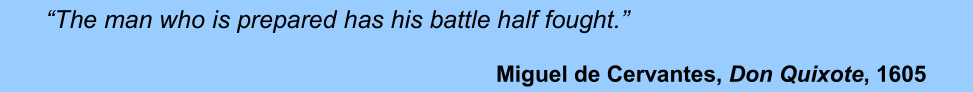
\includegraphics[width=\paperwidth]{quote4.png}}
\end{center}



%
\section{Introduction}

\begin{e1}
	\item La préparation comprend toutes les activités effectuées par l'unité pour améliorer sa capacité à effectuer des opérations, parmi lesquelles: répétitions, mouvements et observations (\fullref{preparation}).
	\item Une fois le plan établi et approuvé, il doit être répété. Cela inclut les circuits de communications primaires et secondaires, et a méthodologie de contrôle. Les observateurs doivent être identifiés et leurs capacités de communication vérifiées. Les mouvements tactiques sur le champ de bataille doivent être pris en compte. \textbf{Le plan dans son ensemble doit être réalisable, exécutable et tactiquement sain}.
	\item La coordination entre les différents échelons et les préparations juste avant l'exécution sont tout aussi importantes que le développement du plan lui même. Pour le Staff, la préparation inclut le rassemblement et la mise à jour constante des estimations (\gls{jipoe})
	\item Se préparer implique des briefings \gls{coe}, des missions de répétition \gls{coe}, l'\gls{opord}, des brief-back, la vérification de l'équipement et des communications, la révision des \glspl{sop}, la vérification du plan de chargement, les vérifications avant-combat, et le test de l'armement.
\end{e1}

\efig{preparation}{Préparation au CAS}
\section{Répétitions}

\note{Dans cette section, le mot ``répéter'' est à prendre au même sens que pour le théâtre, où les acteurs ``répètent'' une scène, et non pas au sens ``répéter'' comme ``dire une seconde fois''}

\begin{e1}
	\item Les répétitions sont l'un des aspects le plus souvent ``oublié'' lors de la préparation d'une mission. Ils offrent à tous les participants l'opportunité de se faire une idée du champ de bataille, s'assurer de la totale compréhension du plan par tous, diminue les temps de réaction de chacun, permet d'identifier les zones d'ombre,d e friction ou de conflit parmi les participants. Le fait de ``voir'' les choses permet de les imprimer en mémoire à plus long terme. Les possibilités de la répétition sont limitées par l'imagination, la situation tactique, le temps et les ressources disponibles.
	\item Les \glspl{sop} devrait identifier les types et techniques de répétitions appropriées, ainsi que les standards pour leur exécution. Cette section se concentre sur les points clefs que les participants au \gls{cas} devraient couvrir, ce dont ils devront discuter, et ce qui devra être compris de tous une fois la répétition terminée.
	\item Répétition Joint
	\begin{e2}
		\item{Intentions du \gls{gc}}{Les intentions du \gls{gc} doivent inclure ses intentions quant au \gls{cas}. Le \gls{gc} est conseillé par son \gls{alo} à propos des menaces, de la disponibilité des appareils des combinaisons d'armement potentielles, pour établir un objectif viable et réalisable. Les \glspl{req} doivent clairement décrire l'effet désiré pour accomplir les intentions du \gls{gc}. Souvent, il n'y a pas d'intention propre au \gls{cas}, simplement, le \gls{cas} s'inscrit dans les intentions de tir générale du \gls{gc}.}
		\itemt{Priorités de tir \gls{cas}}{Les \glspl{pof} pour chaque phase de la mission doivent être établies. Pour une sortie \gls{cas}, une prévision de ``qui'' recevra le \gls{cas}, ``quand'' le \gls{cas} est attendu, ``quel'' est l'effet désiré par le \gls{gc} et ``où'' se trouve les observateurs primaires et secondaires sera nécessaire. De plus, à la fin de la répétition, les participants devront avoir une bonne compréhension de:}
		\begin{e3}
			\item Vérification de la grille de coordonnées ou des position des cibles de grande importance, des observateurs, des unités alliées, et des mouvements prévus (par phase)
			\item Critères déclencheurs pour les cibles et leur engagement
			\item \glspl{fscm} / \glspl{acm} leurs implications pour la manoeuvre
			\item Vérifier le plan \gls{sead}
			\item Connectivité des communications
			\item Vérifier la marque des cibles, et, si d'application, la marque des alliés
			\item Quel \ja{} fournira le \gls{tac} des appareils de \gls{cas}
			\begin{e4}
				\item Disponibilité du \gls{faca}
				\item Plan pour utiliser les sorties \gls{cas} en excès (Killboxes ou dégagement vers un autre secteur ou un autre \gls{faca})
				\item Procédures de collection des \glspl{bda} et des \glspl{misrep}
			\end{e4}
			\item Après la répétition, les participants doivent pouvoir communiquer le plan aux unités subordonnées avant le début de l'opération. Durant la répétition, l'\gls{alo} abordera les points suivants:
			\begin{e4}
				\item Confirmation des intentions du \gls{gc}
				\item Nombre de sorties \gls{cas} prévues
				\item Type d'appareil
				\item Armement embarqué
				\item \gls{cas} \gls{tos}
				\item \glspl{cp} et \glspl{ip}
				\item \glspl{acm} / \glspl{fscm}
				\item Plan \gls{sead}
				\item Marques / plan laser
				\item Procédures de marquages de alliés
				\item \glspl{req} approuvées et \glspl{req} refusées
				\item Types de \gls{tac}
			\end{e4}
		\end{e3}
	\end{e2}
	\item Répétition pour l'appui-feu
	\begin{e2}
		\item Les répétitions de l'appui-feu se concentrent sur la synchronisation des différents appuis-feu. Les points suivants doivent être abordés:
		\begin{e3}
			\item Répéter l'exécution du \gls{cas} avec la manoeuvre des éléments au sol et le \gls{jtac}
			\item Identifier les \glspl{fscm} et confirmer qu'elles apportent un plus au plan de manoeuvre
			\item Vérifier la liste collective des cibles pour s'assurer qu'elle inclut les cibles \gls{cas}
			\item Vérifier les positions des coordonnées pour les cible de grande importance
			\item Vérifier que chaque cible \gls{cas} s'est vue assignée un tasking, un but, une méthode et un effet, et que les priorités \gls{cas} sont clairement définies
			\item Vérifier les critères déclencheurs pour chaque cible et pour chaque engagement
			\item Revoir les \glspl{roe} / \glspl{pid}
			\item Répéter les actions \gls{cas} à effectuer lorsque les critères déclencheurs sont remplis
			\item Répéter les points d'observations primaires et secondaires
			\begin{e4}
				\item Identifier les observateurs primaires et secondaires (\gls{jtac}, \gls{faca}, scout, sniper, etc.)
				\item Identifier les unités de force protection
				\item Identifier les routes d'infiltration / exfiltration
				\item Identifier les critères déclencheurs
				\item Identifier les critères qui initient un déplacement
				\item Revoir les considérations météo
				\item Revoir les procédures de nuit
				\item Confirmer le plan d'observation				
			\end{e4}
			\item identifier les unités alliées les plus proches
			\item Vérifier les procédures de marque des alliés
			\item Voir les tactiques \gls{cas} qui seront probablement utilisée (haute, moyenne, basse, très basse altitude)
			\item Répéter les procédures d'engagement pour les cibles \gls{cas}
			\item Revoir le plan de communication
			\begin{e4}
				\item Confirmer les call-signs
				\item Vérifier les \glspl{jtac} primaires / secondaires
				\item Vérifier les mots-code
				\item Effectuer les radio-check des différents réseaux
				\item Vérifier CRYPTO et procédures \gls{comsec}
				\item Revoir les procédures d'authentification
			\end{e4}
			\item Vérifier le guidage terminal pour chaque cible (unité(s) qui tire(nt), nombre de tirs, quantité et type d'appareils, armement standard)
			\item Vérifier et ``déconflictionner'' le plan de mouvement spécifiant quand et où les unités d'appui-feu vont bouger:
			\begin{e4}
				\item \gls{aof} principal
				\item Zones de prises de position
			\end{e4}
			\item Vérifier la méthode d'engagement (``Sur mon ordre'', \gls{tot}, ou ``Quand prêt'')
			\item \glspl{fscm} / \glspl{acm}
			\begin{e4}
				\item Planning ou ordre pour déplacer les \glspl{fscm}
				\item Formel
				\item Informel
			\end{e4}
			\item Identifier les \glspl{cp} / \glspl{ip} et le flux général des appareils de \gls{cas}
			\item Répéter le plan \gls{sead}
			\item Répéter les procédures de marquage des cibles \gls{cas}
			\begin{e4}
				\item Revoir l'intégration des plan de tirs surface et air
				\item Vérifier les unités \gls{idf} disponibles
				\item Revoir les marques, plan \gls{sead} et méthodes de contrôle
				\item Vérifier les positions des unités \gls{idf}
				\item Vérifier les lignes de tir pour les cibles prévues
			\end{e4}
			\item \gls{tot} / \gls{ttt}
			\item Revoir le type de contrôle pour les cibles \gls{cas}
			\begin{e4}
				\item Type 1, 2 ou 3
				\item Vérifier la connectivité entre les observateurs et les contrôleurs
				\item Revoir la procédure d'autorisation de tir pour les cibles \gls{cas}
			\end{e4}
			\item Faire les ajustement nécessaires
			\item \glspl{fscm} comprises par tous
			\item Discuter des positions \gls{idf}
		\end{e3}
	\end{e2}
\end{e1}
\section{Préparations avant le combat}

\begin{e1}
	\item Les préparations avant le combat permettent au personnel de se préparer pour une mission et donnent au leader une opportunité de s'assurer que le personnel et l'équipement est opérationnel.
	\item La checklist suivante propose un guide pour effectuer cette préparation:
	\begin{e2}
		\itemt{Connaissances essentielles à la mission}{S'assurer que le personnel de chaque élément subordonné comprend la mission, l'objectif et les grandes lignes de la manoeuvre}
		\itemt{Equipement essentiel à la mission}{S'assurer que tout l'équipement est présent et en ordre de fonctionnement. le \gls{jtac} doit prévoir un équipement de communication et un équipement de marquage de rechange.}
		\itemt{Coordination essentielle pour la mission}{S'assurer de la distribution des images ou graphiques dépeignant:}
		\begin{e3}
			\item Grandes lignes de la manoeuvre
			\item \glspl{fscm}
			\item \glspl{acm}
			\item \glspl{nai} et/ou \glspl{tai}
			\item Points de décision et déclencheurs
			\item \glspl{cp} et \glspl{ip} pour les \glspl{fw}
			\item \glspl{ha} et \glspl{bp} pour les \glspl{rw}
			\item Obstacles à la mobilité ou au plan
			\item Procédures de marque de alliés
			\begin{e4}
				\item De jour
				\item De nuit
			\end{e4}
			\item Liste des cibles, graphiques montrant la (zone) cible, chronologie des tirs
			\begin{e4}
				\item \gls{pof} / priorités du \gls{cas}
				\item Cibles prioritaires
				\item Cibles \gls{sead}
			\end{e4}
		\end{e3}
	\end{e2}
\end{e1}
\section{Communications}

\e
    \item Les participants au \gls{cas} utiliseront les réseaux radios des unités qui requièrent le soutien aérien.
    \item
    De façon plus spécifique, les unités capables d'effectuer le \gls{cas} auront besoin des fréquences radios et des call-signs utilisés par les différentes agences, unités au sol, et \glspl{jtac} qu'elles seront susceptibles d'avoir à contacter.
    \item Voici une simplification des différents réseaux radios utilisés lors du \gls{cas} (tous ``voice''):
    \ee
        \item Army Command/Operation Net: réseau utilisé par les \glspl{gc}.
        \item Fire Support Net: réseau utilisé pour les demandes d'appui-feu.
        \item Air Control Net: réseau utilisé par les différentes agences et unités de contrôle pour coordonner les différentes unités sous leur contrôle.
        \item C2Net: interface entre les différentes unités et agences de contrôle.
        \item Guard Net: fréquence de garde; lorsque c'est possible, toute unité engagée en opération sera à l'écoute de ce réseau.
        \item INFLTREP: utilisé pour le \gls{misrep} pendant l'egress
    \ed
\ed

%

\fancyhead[L]{}
\renewcommand{\headrulewidth}{0pt}% Line at the header visible
\newpage
%\vskip2cm
%\begin{minipage}{\linewidth}
\chapter{Exécution}
%\noindent\rule{\textwidth}{0.3pt}
{\center \makebox[\textwidth]{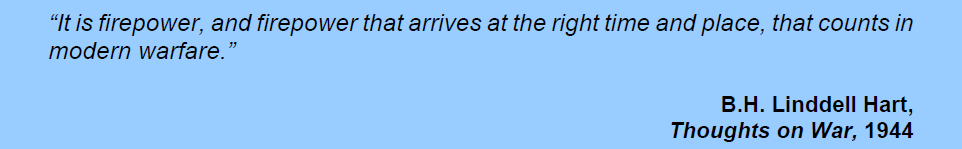
\includegraphics[width=\linewidth]{quote5.png}}}
%\rule{\textwidth}{0.3pt}
%\end{minipage}
\vfill

\newpage
\pagestyle{default}

\section{Introduction}

L'exécution du \gls{cas} commence lorsque la cible est désignée par le \gls{gc} soutenu, et décrit les considérations à prendre en compte pour intégrer le \gls{cas} aux manoeuvres de l'unité soutenue.

\section{Engagement de la cible lors du CAS}

Cette section décrit les procédures standard lors du \gls{cas}. Bien que certaines opérations nécessitent des procédures spécifiques, le personnel impliqué dans le \gls{cas} doit être familier avec le format standard.

\subsection{Création du briefing par le J-TAC}
Cette sous-section décrit les tâches que doit effectuer le \gls{jtac} une fois que la cible a été désignée par le \gls{gc}.

\begin{e1}
	\item Rassembler les informations à propos de la cible
	\begin{e2}
		\itemt{Élévation de la cible (ligne 4)}{
		Par défaut, l'élévation est exprimée en pieds au dessus de la mer (ft \gls{msl})}
		\itemt{Description de la cible (ligne 5)}{
		La description de la cible doit être concise et précise (par ex. ``5 chars dans un champ''). Le \gls{jtac}/\gls{faca} doit éviter d'utiliser des descriptions compliquées ou des termes qui risquent de ne pas être compris par les pilotes. Cependant, la descrition doit rester spécifique. si le \gls{gc} veut attaquer une \gls{hvt} qui se trouve dans un building à deux étages, il devra spécifier "\gls{hvt} dans building à 2 étages", et pas seulement "building à 2 étages".}
		\itemt{Position de la cible (ligne 6)}{
		Le \gls{jtac}/\gls{faca} doit évaluer la précision minimale nécéssaire pour les coordonnées de la cible pour accomplir les objectifs du \gls{gc}. Un largage de bombe guidée laser depuis un émetteur au sol demandera des coordonnées beaucoup moins précises qu'une largage de \gls{jdam}.}
		\begin{e3}
			\itemt{Association du terrain et d'une carte}{
			Le moins précis, mais rapide et efficace en fonction de la situation.}
			\itemt{\gls{lrf} couplé au \gls{gps} et/ou la boussole}{
			Sujet à l'imprécision de la boussole, et au brouillage \gls{gps}. Si le brouillage \gls{gps} est possible, une autre méthode devra être utilisée.}
			\item Logiciel de ciblage
			\item Coordonnées dérivées des images de reconnaissance
		\end{e3}
		\itemt{Positions alliées (ligne 8)}{
		La positions des unités alliées au sol sont données à partir de la position de la cible. La direction est donnée de manière cardinale ou sous-cardinale, et la distance est exprimée en mètres. L'observateur ou le \gls{jtac} peuvent ne pas être l'unité alliée la plus proche de la cible.}
		\itemt{Effet souhaité par le \gls{gc}}{
		L'effet souhaité par le \gls{gc} est déterminé en parlant avec lui. Le \gls{jtac} doit offrir au \gls{gc} une estimation réaliste des possibilités en fonction des appareils disponibles, de l'armement embarqué, et de son expertise.}
	\end{e2}
\end{e1}
\subsection{Requête de CAS}
\begin{e1}
	\item Une fois que la position de la cible a été grossièrement estimée, le \gls{jtac} doit envoyer la demande de \gls{cas} le plus vite possible, pour prendre en compte le temps nécessaire avant l'arrivée des appareils. Il ne faut pas retarder l'envoi de la demande pour augmenter la précision des coordonnées de la cible.\\ \important{Il ne faut jamais utiliser les coordonnées des unités alliées comme coordonnées cible dans une demande de \gls{cas}.}
	\itemt{Création du game plan}{
	Au minimum, le game plan contiendra le type de contrôle et la méthode d'attaque. D'autres informations peuvent être intégrée au game plan ou être ajouté plus tard aux remarques du CAS brief: les intentions du \gls{gc}, l'effet désiré, l'intervalle entre les appareils dans le cas d'une attaque simultanée par plusieurs éléments \gls{cas}. Dans le cas d'attaques séquentielles (\gls{sead}, marquage), une attention particulière devra être apportée à l'établissement de la séparation entre les appareils. L'objectif du \gls{jtac} n'est pas de dicter aux appareils de \gls{cas} les tactiques à employer, mais de fournir un plan qui correspond aux intentions du \gls{gc}.}
	\begin{e2}
		\itemt{Déterminer l'effet désiré}{}
		\remark{
		\begin{e3}
			\item Composition de la cible (blindage)
			\item Répartition de la cible (centré sur un point ou dispersé)
			\item Position (dégagée ou protégée)
			\item Dégâts collatéraux potentiels
			\item Proximité des unités alliées
		\end{e3}
		}
		\itemt{Choisir le type de \gls{tac}}{
		Le type de \gls{tac} dépend de l'armement employé, de la manière manière de réduire les risques, de la vitesse de l'engagement et de la capacité du \gls{jtac} à voir la cible et/ou l'appareil qui attaque.}
		\itemt{Choisir la méthode d'attaque (\gls{boc} ou \gls{bot})}{
			La méthode d'attaque est choisie de manière à permettre l'attaque la plus rapide possible, en fonction du type de cible, de la façon dont sera acquise la cible, et de la situation}
		\itemt{Planifier l'intervalle entre les appareils}{
		Le \gls{jtac} peut demander un intervalle spécifique entre les attaques, en fonction de la cible, des menaces, des activités alliées, de la déconfliction artillerie/\gls{sead}/laser, de l'armement utilisé, des restrictions, de la météo, etc. Les pilotes se doivent d'adapter leur tactiques pour respecter le timing et les intervalles imposés.}
		\begin{e3}
			\itemt{Attaque simultanée}{
			Tous les appareils délivreront leur armement de manière à créer un effet simultané. Cette méthode minimise l'exposition des appareils aux menaces et offre à l'ennemi un temps de réaction très court. C'est la méthode optimale pour engager des cibles multiples, tout particulièrement des cibles mobiles qui pourraient fuir après la première attaque. Le principal désavantage de cette méthode est l'impossibilité de corriger ou d'annuler le tir entre les impacts et la diminution du support mutuel entre les appareils qui attaquent.\\
			\important{Un attaque simultanée nécessite que les appareils utilisent des codes laser différents.}}
			\itemt{Attaque séquentielle}{
			Les appareils attaquent un à la fois, avec un intervalle spécifique entre les attaques, basé sur le temps nécessaire à l'acquisition de l'appareil précédent, la durée de vol de l'arme employée, le temps nécessaire au dégagement visuel de la zone attaquée (fumée, fragments, etc.), et le temps nécessaire à évaluer l'efficacité de la frappe précédente et le besoin d'une nouvelle frappe.\\ Quelques guides pour les attaques séquentielles:}
			\begin{e4}
				\item 30 secondes pour un contrôle de \gls{typeone} avec des bombes lisses
				\item 1 minute pour des \gls{lgb} délivrées à altitude moyenne
				\item Plus de deux minutes pour décider de la ré-attaque lors de l'emploi de \gls{pgm} à haute ou moyenne altitude
			\end{e4}
		\end{e3}
	\end{e2}
	\item Détermination du type de marque et de l'aide à la corrélation
	\begin{e2}
		\itemt{\gls{boc}}{
		\begin{e3}
			\item Pas de marque nécessaire (ligne 7: "No mark")
			\item Si le \gls{tac} est utilisé avec des \gls{lgw}, le call-sign de l'unité qui fournit le \gls{tac} et le code laser seront fournis.\\ (ligne 7 (exemple): "Blackjack laser, code 1688")
		\end{e3}}
		\itemt{\gls{bot}}{
		La marque dépendra de l'appareil qui attaque}
		\item \gls{bot} et contribution d'une tierce partie
		\begin{e3}
			\itemt{Tierce partie}{
Suite l'expansion des technologies déployées sur le champ de bataille, le \gls{jtac} peut décider de recourir à une tierce partie (unité \gls{recce}, sniper, appareils équipés d'un émetteur laser, etc.) pour aider à l'obtention des coordonnées ou de la position de la cible, à l'attaque terminale ou à l'établissement du \gls{bda}. De ce fait, la corrélation avec ces parties tierces sera également nécessaire.}
\item Considérations
			\begin{e4}
				\item Les pilotes utilisent généralement une combinaison de senseurs et leurs yeux pour acquérir les marques et les cibles. Le \gls{jtac} doivent être familiers avec les capacités des senseurs et utiliser des marques qui utilisent ces capacités.
				\item Le \gls{jtac} doit toujours avoir en réserve un plan de marquage alternatif.
			\end{e4}
			\item Types de marque et \gls{tgo}
			\begin{e4}
				\itemt{Marquage laser}{
				Le passage de la marque laser est le fait d'utiliser un \gls{ltd} pour fournir l'énergie laser au \gls{lst} de l'appareil. Le \gls{ltd} peut se trouver au sol ou embarqué dans un autre appareil.}
				\begin{e5}
					\item Avantages
					\begin{e6}
						\item Excellente corrélation de la position de la cible si la géométrie correcte est utilisée
						\item Peut être utilisé de jour comme de nuit
					\end{e6}
					\item Désavantages
					\begin{e6}
							\item Nécessite un \gls{ltd} et un \gls{lst}
							\item Demande de la coordination géométrique pour le \gls{lst} ne traque pas le \gls{ltd} (l'origine du pointage)
							\item Le marquage laser depuis le sol est souvent difficile, particulièrement lorsque l'unité qui effectue le pointage est sous le feu ennemi
							\item Un premier passage d'acquisition de la marque est parfois nécessaire
					\end{e6}
					\important{Lors du marquage laser depuis le sol, un \gls{fah} sera obligatoirement donné, de manière à renforcer l'établissement de la géométrie correcte}
				\end{e5}
				\itemt{Marquage infrarouge (\acrshort{sparkle})}{
				Les pilotes utiliseront leur \gls{nvg} pour acquérir la cible.}
				\important{Les pilotes doivent appeler "VISUEL SPARKLE", "TALLY SPARKLE" ou "CONTACT SPARKLE" quand un marquage infrarouge est utilisé à partir du sol}
				\begin{e5}
					\item Avantages
					\begin{e6}
						\item Rapide
						\item Le \gls{jtac} a la confirmation visuelle que le pilote a bien acquis la cible correcte							
					\end{e6}
					\item Désavantages
					\begin{e6}
						\item De nuit seulement
						\item Requiert de la coordination géométrique pour s'assurer que le pilote a bien acquis la fin du faisceau infrarouge et non pas sa source
						\item S'il y a plusieurs pointeurs \gls{ir} près d'une même cible, il devient difficile pour le \gls{jtac} de déterminer si le pointeur se trouve bien sur la cible à cause du phénomène de ``diffusion'' dans les \gls{nvg}
						\item Si l'ennemi dispose également de \gls{nvg}, l'utilisation d'\gls{ir} expose l'opérateur et supprime le facteur de surprise
					\end{e6}
				\end{e5}
				\itemt{Marquage à partir d'un \gls{trp}}{}
				\begin{e5}
					\item Avantages
					\begin{e6}
						\item Prêt rapidement si le pilote connaît le \gls{trp}
						\item De jour comme de nuit
						\item Offre un point de référence commun pour le talk-on
					\end{e6}
					\item Désavantages
					\begin{e6}
						\item Nécessite le pilote connaisse le \gls{trp}
					\end{e6}
				\end{e5}
				\itemt{Marquage \gls{idf} (fumigène)}{}
				\begin{e5}
					\item Avantages
					\begin{e6}
						\item De jour comme de nuit (obus phosphorescents ou lumineux)
						\item Le \gls{jtac} ne doit pas dévoiler sa position
						\item Offre un point de référence commun pour le talk-on
					\end{e6}
					\item Désavantages
					\begin{e6}
						\item Prend du temps à coordonner
						\item Le manque de précision implique souvent une correction supplémentaire à partir de la marque
						\item Le tire indirect implique une déconfliction supplémentaire
						\item Le \gls{fov} des senseurs peut être un problème si la marque se trouve en dehors
						\item L'illumination de nuit sature les \gls{nvg}
						\item Sacrifie l'effet de surprise
					\end{e6}
				\end{e5}
				\itemt{Marquage par feu direct}{
				Utilise un tir direct (munitions traçantes ou grandes fumigènes) pour marquer la cible.}
				\begin{e5}
					\item Avantages
					\begin{e6}
						\item Facilement accessible
					\end{e6}
					\item Désavantages
					\begin{e6}
						\item Risque de dommages collatéraux
						\item Difficulté pour les \gls{rw} d'acquérir visuellement la marque de jour
						\item Difficulté pour les \gls{fw} d'acquérir visuellement la marque de jour comme de nuit
						\item Le \gls{fov} des senseurs peut être un problème si la marque se trouve en dehors
						\item L'illumination de nuit sature les \glspl{nvg}
						\item Sacrifie l'effet de surprise
					\end{e6}
				\end{e5}
				\itemt{Considérations pour le marquage de nuit}{}
				\begin{e5}
					\item La visibilité limitée et le manque de perspective rend la corrélation de nuit difficile
					\item L'illumination du champ de bataille doit être planifiée de manière à ne pas saturer les \glspl{nvg}
				\end{e5}
				\itemt{Marques d'opportunité}{
				N'importe quoi sur le champ de bataille peut servir de marque; un bâtiment en feu, le trafic routier, etc.}
			\end{e4}
	   	\end{e3}
	\end{e2}
	\item Détermination la géométrie d'attaque reprise 227 %TODO
\end{e1}
%	\begin{figure}[H]
%		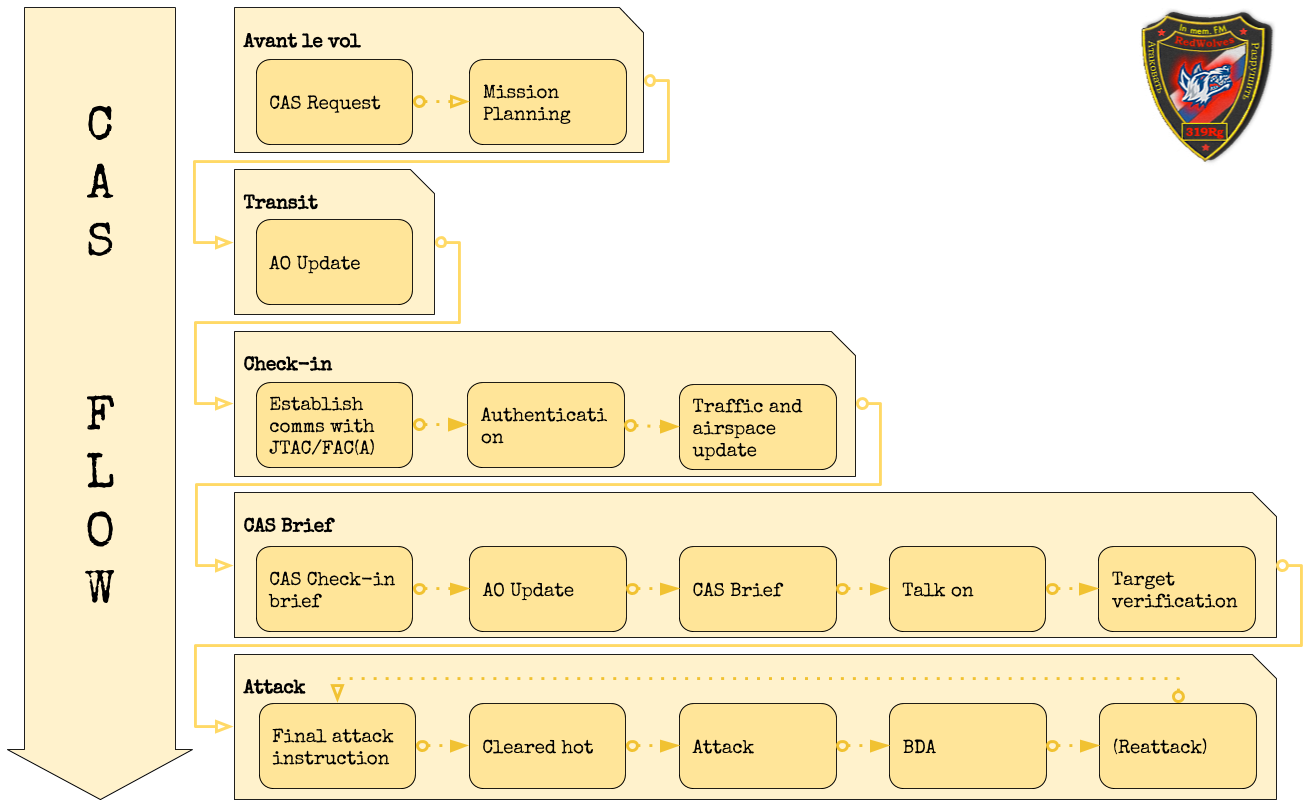
\includegraphics[width=\textwidth]{CASFlow.png}
%		\caption{Cas flow simplifié.}
%		\label{fig:casflow}
%	\end{figure}
	\begin{figure}[H]
		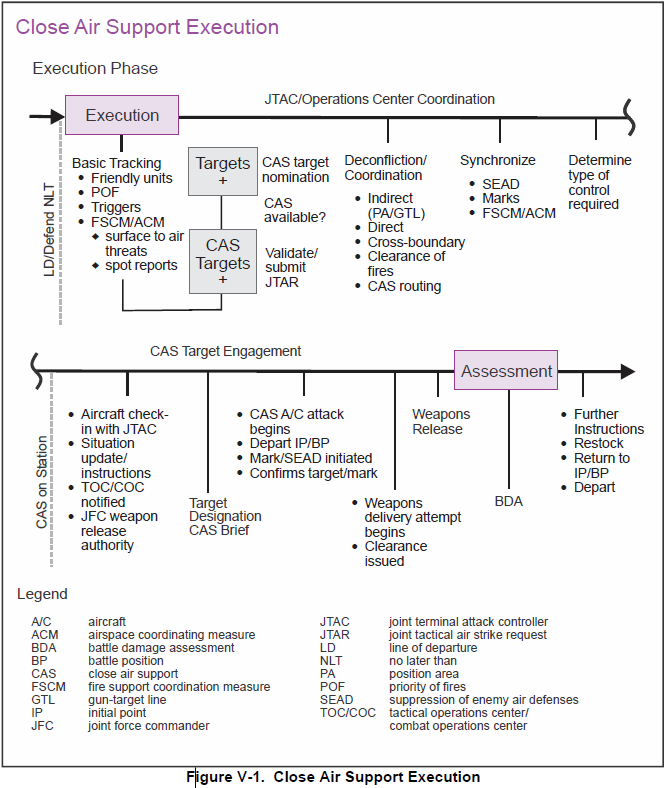
\includegraphics[width=\textwidth]{execution-full.png}
		\caption{Cas flow réel.}
		\label{fig:casflow-full}
	\end{figure}
\begin{figure}[H]
\begin{tikzpicture}
  \tikzstyle{every node}=[font=\footnotesize]
  \matrix[column sep=0.5cm, row sep=1.4cm]
  {
	\node [process] (req)		  {CAS request};&
	\node [process] (planning)	 {Mission planning};\\
	
	\node [process] (aoupdate)	 {AO Update};\\
	
	\node [process] (comms)		{Establish comms with J-TAC/\\FAC(A)}; &%
	\node [process] (auth)		 {Authent-\\ication};&%
	\node [process] (tfcupd)	   {Traffic and airpsace update};\\%
	
	\node [process] (ci) {Check-in brief};&
	\node [process] (aoupd2)	   {AO update};&
	\node [process] (casbrief)	 {CAS brief};&
	\node [process] (talkon)	   {Talk-on};&
	\node [process] (corr)		 {Target correlation};\\
	
	\node [process] (fai)		  {Final attack instructions};&
	\node [process] (ch)		   {Cleared hot};&
	\node [process] (attack)	   {Attack};&
	\node [process] (bda)		  {BDA};&
	\node [process] (reattack)	 {Re-attack};\\
  };
  	\begin{pgfonlayer}{background}
		\node [fill=orange!30, fit={($(req.west)	 -(0.2cm,0)$)([yshift=0.6cm]req.north)([yshift=-0.2cm]req.south)([xshift=0.2cm]planning.east)}] (preflightbg) {};
		\node [fill=orange!30, fit={($(aoupdate.west)-(0.2cm,0)$)([yshift=0.6cm]aoupdate.north)([yshift=-0.2cm]aoupdate.south)([xshift=0.2cm]aoupdate.east)}] (aoupdatebg) {};
		\node [fill=orange!30, fit={($(comms.west)   -(0.2cm,0)$)([yshift=0.6cm]comms.north)([yshift=-0.2cm]comms.south)([xshift=0.2cm]tfcupd.east)}] (checkinbg) {};
		\node [fill=orange!30, fit={($(ci.west)	  -(0.2cm,0)$)([yshift=0.6cm]ci.north)([yshift=-0.2cm]ci.south)([xshift=0.2cm]corr.east)}] (casbriefbg) {};
		\node [fill=orange!30, fit={($(fai.west)	 -(0.2cm,0)$)([yshift=0.6cm]fai.north)([yshift=-0.2cm]fai.south)([xshift=0.2cm]reattack.east)}] (attackbg) {};
	\end{pgfonlayer}
	
	\node [text centered, anchor=north west, font=\bfseries, yshift=0cm] at (preflightbg.north west) {Avant le vol};
	\node [text centered, anchor=north west, font=\bfseries, yshift=0cm] at (aoupdatebg.north west) {Transit};
	\node [text centered, anchor=north west, font=\bfseries, yshift=0cm] at (checkinbg.north west) {Check-in};
	\node [text centered, anchor=north west, font=\bfseries, yshift=0cm] at (casbriefbg.north west) {CAS brief};
	\node [text centered, anchor=north west, font=\bfseries, yshift=0cm] at (attackbg.north west) {Attaque};
	
	\draw [my arrow] (req.east)	  -- (planning.west);
	\draw [my arrow] (comms.east)	-- (auth.west);
	\draw [my arrow] (ci.east)	   -- (aoupd2.west);
	\draw [my arrow] (aoupd2.east)   -- (casbrief.west);
	\draw [my arrow] (casbrief.east) -- (talkon.west);
	\draw [my arrow] (talkon.east)   -- (corr.west);	
	\draw [my arrow] (auth.east)	 -- (tfcupd.west);	
	\draw [my arrow] (fai.east)	  -- (ch.west);
	\draw [my arrow] (ch.east)	   -- (attack.west);
	\draw [my arrow] (attack.east)   -- (bda.west);
	\draw [my arrow] (bda.east)	  -- (reattack.west);
	\draw[ultra thick, orange, ->] (planning.east) -- ++ (1cm,0) |- ($(aoupdate.north west)-(1cm,-0.9cm)$) |- (aoupdate.west);
	\draw[ultra thick, orange, ->] (aoupdate.east) -- ++ (1cm,0) |- ($(comms.north west)   -(1cm,-0.9cm)$) |- (comms.west);
	\draw[ultra thick, orange, ->] (tfcupd.east)   -- ++ (1cm,0) |- ($(ci.north west)	  -(1cm,-0.9cm)$) |- (ci.west);
	\draw[ultra thick, orange, ->] (corr.east)	 -- ++ (1cm,0) |- ($(fai.north west)	 -(1cm,-0.9cm)$) |- (fai.west);
	\draw[ultra thick, orange, ->] (reattack.south) -- ++ (0,-0.5cm) |- ($(fai.south)-(0,0.5cm)$) -- (fai.south);
\end{tikzpicture}
\caption{Cas flow simplifié.}
\label{fig:casflow} 
\end{figure}

%\begin{tikzpicture}[domain=0:4] 
%	\draw[very thin,color=gray] (-0.1,-1.1) grid (3.9,3.9);
%	\draw[->] (-0.2,0) -- (4.2,0) node[right] {$x$}; 
%	\draw[->] (0,-1.2) -- (0,4.2) node[above] {$f(x)$};
%	\draw[color=red]	plot (\x,\x)			 node[right] {$f(x) =x$}; 
%	\draw[color=blue]   plot (\x,{sin(\x r)})	node[right] {$f(x) = \sin x$}; 
%	\draw[color=orange] plot (\x,{0.05*exp(\x)}) node[right] {$f(x) = \frac{1}{20} \mathrm e^x$};
%  \end{tikzpicture}

\begin{e1}
	\item
	Ce chapitre présente le déroulement pratique d’une mission \acrshort{cas}. Le template qui y est présenté illustre une mission \acrshort{cas} typique, et fournit un guide pour le \acrshort{jtac}/\acrshort{faca} et le pilote pour les aider à remplir leur mission.
	\item Le déroulement présenté ici commence après le décollage, et se termine lorsque la patrouille de \acrshort{cas} est sur le retour.
\end{e1}

\section{Routing}
\begin{e1}
	\item Le routing consiste à diriger les appareils d’un point à un autre.
	\item Extrait du \jp:\\
	\begin{figure}[H]
		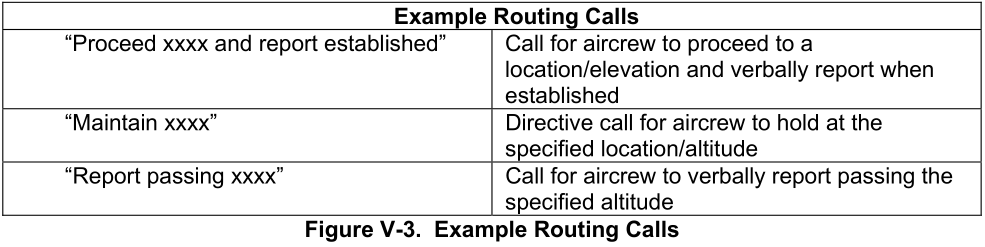
\includegraphics[width=\textwidth]{routing.png}
		\caption{Routing.}
		\label{fig:routing}
	\end{figure}
	\item Exemples:\\
\end{e1}

\section{Check-in}

\begin{e1}
	\begin{minipage}{\linewidth}
	\item
	Le check-in est la première phase du \acrshort{cas} en tant que tel. C’est l’appel effectué de l’appareil en \acrshort{cas} vers le \acrshort{jtac}/\acrshort{faca} pour lui signifier qu’il est prêt à remplir sa mission de \acrshort{cas}.
	\item Comme le check-in peut prendre un certain temps, un appel préliminaire devrait être effectué. Par exemple:
	\begin{lstlisting}[caption=Appel préliminaire, label=preliminary_call]
	PIRATE, ici REDWOLF, pour check-in, quand dispo.
	\end{lstlisting}
	\end{minipage}

	\begin{minipage}{\linewidth}
	\item Format du check-in:
	\begin{figure}[H]
		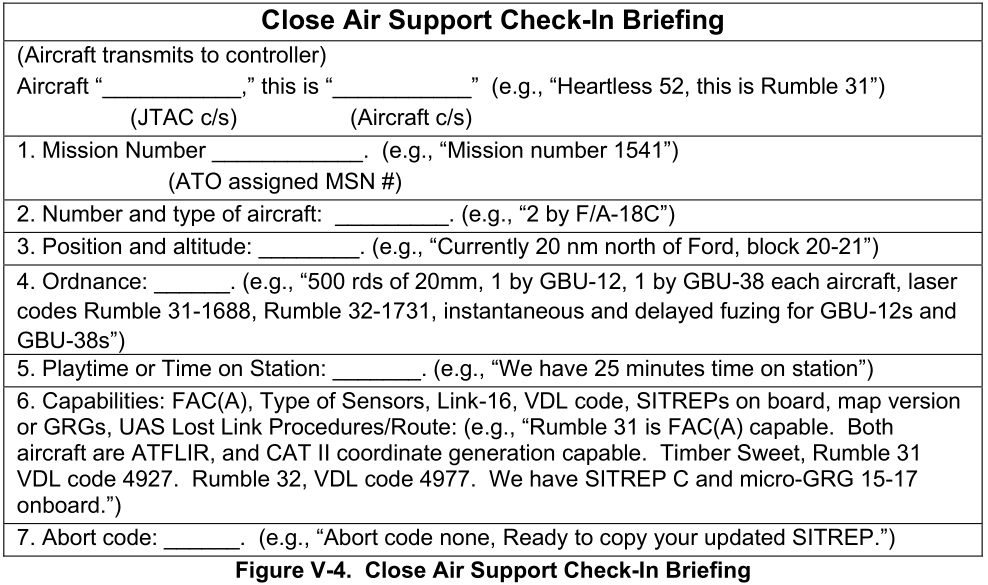
\includegraphics[width=\textwidth]{checkin.png}
		\caption{Format check-in.}
		\label{fig:checkin}
	\end{figure}	
	\end{minipage}
	
	\begin{minipage}{\linewidth}
	\item S'il le souhaite, le \gls{jtac}/\gls{faca} peut demander un check-in abrégé:
	\begin{figure}[H]
		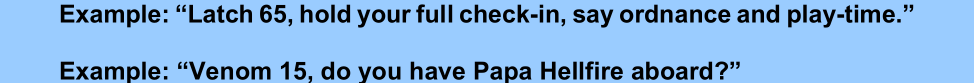
\includegraphics[width=\textwidth]{abbregcheckin.png}
		\caption{Format check-in abrégé.}
		\label{fig:abbregcheckin}
	\end{figure}
	\end{minipage}
	
	\item Le code d’annulation (ligne 7) est un code alphabétique servant à authentifier la directive ``Abort'' du J-TAC/FAC(A).
	
	\begin{minipage}{\linewidth}
	\item Exemple de check-in:
	\begin{lstlisting}[caption=Check-in, label=checkin]
	PIRATE ici REDWOLF
		Mission 1234
		2 Kamov
		20km au sud de Poti, 500m MSL
		24 Vikhrs, 80 roquettes, full guns
		Playtime 30 minutes
		Senseurs: Shkval
		Abort code: X-RAY TANGO ZULU
	\end{lstlisting}
	\end{minipage}
\end{e1}
%
%
\newpage%
%
\pagestyle{intro}%
%
%\pagenumbering{Roman}%
%
\microtypesetup{protrusion=false}%
%
\invisibleunnumberedchapter{Listes}%
%
\invisibleunnumberedsection{Liste des images}%
\makeatletter%
\@starttoc{lof}% Print List of Figures
\makeatother%
%
\newpage%
%
\invisibleunnumberedsection{Liste des tableaux}%
\makeatletter%
\@starttoc{lot}% Print List of Figures
\makeatother%
%
%\phantomsection
%%\addcontentsline{toc}{chapter}{\listtablename}
%\addtocontents{lot}{\protect\addcontentsline{toc}{chapter}{Liste des tables}}
%\listoftables
%
\newpage%
%
\invisibleunnumberedsection{Liste des exemples}%
\makeatletter%
\@starttoc{lol}% Print List of Figures
\makeatother%
%
\newpage%
\invisibleunnumberedsection{Points à traiter}%
\listoftodos
%
%\phantomsection
%%\addcontentsline{toc}{chapter}{\lstlistlistingname}
%\addtocontents{lol}{\protect\addcontentsline{toc}{chapter}{Liste des exemples}}
%\lstlistoflistings{}
%
\microtypesetup{protrusion=true}%
%
\newpage%
%
\invisibleunnumberedchapter{Glossaire}%
%
\glsaddall%
\glossarystyle{altlist}%
\invisibleunnumberedsection{Acronymes}%
%\printglossary[title=Acronymes, toctitle=Acronymes, type=\acronymtype]
\printglossary[type=\acronymtype]
%
\newpage%
%
\invisibleunnumberedsection{Explications des termes}%
\printglossary[type=main]
%
\clearpage%
%
\pagestyle{annexes}%

\begin{appendices}%
%	
\pagestyle{annexes}%

%\chapter{Guide de préparation de mission}\label[annex]{ann1}
%\chapter{\texorpdfstring{}{Annexe \Alph{chapter} Guide de préparation de mission}}\label[annex]{ann1}
\invisiblechapter{Préparation de mission}\label[annex]{ann1}

\section{Aperçu CAS}

\begin{e1}
    \item Situation alliée
    \begin{e2}
        \item FLOT
        \item \acrfull{cp} / \acrfull{ip}
        \item Grandes lignes de la manoeuvre
        \begin{e3}
            \item Zone cible
            \item Terrain
            \item Position et call-sign \ja{}
            \item Unités de support
            \begin{e4}
            	\item Position et portée de l'artillerie
            	\item Position et portée des mortiers
            	\item Lignes de tir \acrfull{idf}
            \end{e4}
            \item Mesures de contrôle et de coordination
            \begin{e4}
				\item \acrfull{cfl}            %TODO
            \end{e4}
        \end{e3}
        \item Dispositif allié
        \begin{e3}
            \item Zone d’opération
            \item Type de terrain
            \item Position et callsigns du J-TAC/FAC(A)
            \item Unités alliées en support
        \end{e3}
        \item Contrôle et coordination
        \begin{e3}
            \item Mesures permissives
            \item Mesures restrictives
        \end{e3}
        \item Gestion de l’espace aérien
        \item Zones d’engagement de la chasse
    \end{e2}
    \item Situation ennemie
    \begin{e2}
        \item Position et force de l’ennemi
        \begin{e3}
            \item Intention supposée
            \item Route de déplacement probable
            \item Tactiques déjà observées
        \end{e3}
        \item Éléments de support ennemis
        \item Menaces
        \begin{e3}
            \item Position
            \item Type de guidage
            \begin{e4}
                \item Infrarouge
                \item Radar
                \item Optique
            \end{e4}
            \item Capacité de la menace (portée, puissance)
            \item Éléments révélateurs
            \item Tactiques déjà observées
        \end{e3}
    \end{e2}
    \item Météo
    \begin{e2}
        \item Plafond
        \item Visibilité
        \item Température
        \item Vent
    \end{e2}
    \item Environnement
    \begin{e2}
        \item Élévation et azimuth du soleil
        \item Lever et coucher du soleil
    \end{e2}
    \item Objectifs de mission
    \begin{e2}
        \item Objectifs globaux de l’opération
        \item Objectifs du haut commandement
        \item Objectifs de la sortie
        \item Objectifs des unités alliées
        \item Ordre de priorité des différentes cibles potentielles
        \item Heure d’arrivée prévue/imposée sur objectif
        \item Règles d’engagement
    \end{e2}
\end{e1}




%
%
%\chapter{Carte de mission}\label[annex]{ann2}
\invisiblechapter{Carte de mission}\label[annex]{ann2}

\emptypage

%\newpage

\thispagestyle{logoonly}

%\begin{smini}
\begin{adjustbox}{width={\textwidth},totalheight={\textheight}}%
\renewcommand{\arraystretch}{5}
\setlength{\extrarowheight}{-25pt}
{\footnotesize
\noindent
\begin{tabularx}{\textwidth}{ @{} p{\linewidth} @{} }

	{\begin{tabularx}{\textwidth}{@{} X X @{}}
		\textbf{Mission} & Date
	\end{tabularx}}\\ \midrule
	
	\multicolumn{1}{c}{\textbf{Wx}}\\[-3ex] \midrule
	{\begin{tabularx}{\textwidth}{@{} *{7}X @{}}
		Vis & Ceil & Cov & Wind & QNH & Temp & ATIS
	\end{tabularx}}\\ \midrule
	
	{\begin{tabularx}{\textwidth}{@{} X | X @{}}
		{\begin{tabularx}{\linewidth}{@{} X X @{}}
			\multicolumn{2}{c}{\textbf{Fuel}}\\[-3ex] \midrule
			Joker & Bingo\\
		\end{tabularx}} &
		{\begin{tabularx}{\linewidth}{@{} X X @{}}
			\multicolumn{2}{c}{\textbf{Loadout}}\\[-3ex] \midrule
			Int & Ext\\
		\end{tabularx}}
	\end{tabularx}}\\ \midrule
	
	\multicolumn{1}{c}{\textbf{Dep/Rec}}\\[-3ex] \midrule
	{\begin{tabularx}{\textwidth}{@{} *{7}X @{}}
		Airbase & Gnd & Twr & App & Lat & Long & Remarks\\[-3ex] \midrule
		\hfill & \hfill & \hfill & \hfill & \hfill & \hfill & \hfill\\ \midrule
		\hfill & \hfill & \hfill & \hfill & \hfill & \hfill & \hfill\\ \midrule
		\hfill & \hfill & \hfill & \hfill & \hfill & \hfill & \hfill\\
	\end{tabularx}}\\ \midrule
	
	\multicolumn{1}{c}{\textbf{Comms}}\\[-3ex] \midrule
	{\begin{tabularx}{\textwidth}{@{} *{2}X @{}}
		Pri & Sec\\[-3ex]
	\end{tabularx}}\\ \midrule
	{\begin{tabularx}{\textwidth}{@{} X | X @{}}
		{\begin{tabularx}{\linewidth}{@{} *{3}X @{}}
			Callsign & Role & Freq\\[-3ex] \midrule
			\hfill & \hfill & \hfill\\ \midrule
			\hfill & \hfill & \hfill\\ \midrule
			\hfill & \hfill & \hfill\\ \midrule
			\hfill & \hfill & \hfill\\
		\end{tabularx}} &
		{\begin{tabularx}{\linewidth}{@{} *{3}X @{}}
			Callsign & Role & Freq\\[-3ex] \midrule	
			\hfill & \hfill & \hfill\\ \midrule
			\hfill & \hfill & \hfill\\ \midrule
			\hfill & \hfill & \hfill\\ \midrule
			\hfill & \hfill & \hfill\\
		\end{tabularx}}\\
	\end{tabularx}}\\ \midrule
	
	\multicolumn{1}{c}{\textbf{Points}}\\[-3ex] \midrule
	{\begin{tabularx}{\textwidth}{@{} X | X @{}}
		{\begin{tabularx}{\linewidth}{@{} *{4}X @{}}
			Denom & Action & Lat & Long\\[-3ex] \midrule
			\hfill & \hfill & \hfill & \hfill\\ \midrule
			\hfill & \hfill & \hfill & \hfill\\ \midrule
			\hfill & \hfill & \hfill & \hfill\\ \midrule
			\hfill & \hfill & \hfill & \hfill\\ \midrule
			\hfill & \hfill & \hfill & \hfill\\ \midrule
			\hfill & \hfill & \hfill & \hfill\\
		\end{tabularx}} &
		{\begin{tabularx}{\linewidth}{@{} *{4}X @{}}
			Denom & Action & Lat & Long\\[-3ex] \midrule
			\hfill & \hfill & \hfill & \hfill\\ \midrule
			\hfill & \hfill & \hfill & \hfill\\ \midrule
			\hfill & \hfill & \hfill & \hfill\\ \midrule
			\hfill & \hfill & \hfill & \hfill\\ \midrule
			\hfill & \hfill & \hfill & \hfill\\ \midrule
			\hfill & \hfill & \hfill & \hfill\\
		\end{tabularx}}\\
	\end{tabularx}}\\ \midrule
	{\begin{tabularx}{\textwidth}{@{} p{4cm} | X @{}}
		\begin{tabular}[t]{@{} l @{}}
			\multicolumn{1}{c}{\textbf{FENCE IN}}\\[-3ex] \midrule
			Fuel\\[-3ex]
			Emitters\\[-3ex]
			Navigation\\[-3ex]
			Communications\\[-3ex]
			ECM\\[-3ex]
			\midrule
			\multicolumn{1}{c}{\textbf{Menaces}}\\[-3ex] \midrule
			{\begin{tabularx}{\linewidth}{@{} r X X @{}}
				& \textbf{Hor} & \textbf{Ver}\\[-3ex] \midrule
				SA18 & 5k & 3k\\[-3ex] \midrule
				SA9 & 4.2k & 3.5k\\[-3ex] \midrule
				SA13 & 5k & 3.5k\\[-3ex] \midrule
				ZU23 & 2.5k & 2k\\[-3ex] \midrule
				Shilka & 2.5k & 2k\\[-3ex] \midrule
			\end{tabularx}}
		\end{tabular} &
		\textbf{Remarques}\\
	\end{tabularx}}\\
\end{tabularx}
}
%}
%\end{smini}
\end{adjustbox}%%
%
\pagestyle{annexes}%

%\chapter{Requêtes CAS Joint}\label[annex]{annc}
\invisiblechapter{Requêtes CAS Joint}\label[annex]{annexc}

\note{Le format a été adapté pour mieux convenir à l'utilisation qu'on en ferait dans DCS.}

\section{Requête de mission}

\begin{e2}[0em]
	\item Ligne 1 - Heading
	\begin{e3}[0em]
		\item Unité appelée - Destinataire de la requête
		\item Unité appelante - Source de la requête
		\item Numéro de la requête
		\begin{e4}[0em]
			\item CAS planifié - Numérotation séquentielle par l'unité appelante
			\item CAS immédiat - Numérotation séquentielle par le centre ops
		\end{e4}
		\item Envoyé - Date et heure de l'envoi, personne qui a envoyé la requête
	\end{e3}
	\item Ligne 2 - Priorité
	\begin{e3}[0em]
		\item Priorité
		\begin{e4}[0em]
			\item Urgente
			\item Priorité
			\item Routine
		\end{e4}
	\end{e3}
	\itemt{Ligne 3 - Cible}{
	Décrit la composition, la force approximative et les capacités de mouvement de la cible. Il est obligatoire de spécifier, même s'il s'agit d'une grossière estimation, la force de l'ennemi (par ex.: 10 chars) ou la taille de la zone cible (par ex: personnel sur le une ligne de 500 mètres).}
	\item Ligne 4 - Position de la cible
	\begin{e3}[0em]
		\item Bloc A - Position de la cible ou point de départ
		\item Bloc B - Quand indiqué, renseigne une ligne de A vers B
		\item Bloc C - Quand indiqué, renseigne une route qui part de A et qui va vers C en passant par B
		\item Bloc D - Renseigne une route A-B-C-D ou indique une zone dont les coins sont A, B, C et D
		\item Bloc E - Élévation de la cible en \gls{ft} \gls{msl}
	\end{e3}
	\itemt{Ligne 5 - Heure / date}{Indique l'heure et la date auxquelles le \gls{cas} est requis}
	\begin{e3}[0em]
		\item Bloc A - \acrshort{asap}: le plus vite possible
		\item Bloc B - \acrshort{nlt}: pas plus tard que \ldots{}
		\item Bloc C - A: A \ldots{}
		\item Bloc D - To: Jusque \ldots{}
	\end{e3}
	\itemt{Ligne 6 - Armement/Effet désiré}{Indique l'effet souhaité par le demandeur. Cette information est essentielle pour le planificateur.}
	\begin{e3}[0em]
		\item Armement - type d'armement à employer
		\item Détruire
		\item Neutraliser
		\item Harceler/Interdire
	\end{e3}
	\itemt{Ligne 7 - Contrôle final}{Identité du \gls{tac} (ex: \gls{jtac}, \gls{faca}) qui effectuera le briefing et contrôlera le tir}
	\begin{e3}[0em]
		\item JTAC - Type de contrôle terminal
		\item Call-sign
		\item Fréquence tu contrôleur
		\item Point de contrôle - Point auquel le pilote doit contacter le contrôleur
	\end{e3}
	\itemt{Ligne 8 - Remarques}{Permet d'ajouter des informations qui ne sont reprises dans les points ci-dessus dans une ``Situation Update''.}
	\begin{e3}[0em]
		\item Numéro de l'update
		\item Situation de la cible et de l'ennemi
		\item Activités des menaces
		\item Situation alliée
		\item Positions des alliés
		\item Activité de l'artillerie
		\item Autorité pour le \gls{tac}
		\item Armement souhaité
		\item Restrictions / remarques
		\item Effort \gls{sead} localisé
		\item Dangers (météo, terrain)
	\end{e3}
\end{e2}

\section{Coordination}

\begin{re2}
	\item Ligne 9 - \gls{nsfs} - Coordination avec les unités navales
	\item Ligne 10 - Artillerie - Coordination avec l'artillerie
	\item Ligne 11 - Espionnage - Coordination avec les unités de renseignement
	\item Ligne 12 - Requête -  indique si la requête est approuvée
	\item Ligne 13 - Par - indique l'autorité qui a approuvé ou désapprouvé la requête
	\item Ligne 14 - Raison pour la désapprobation
	\item Ligne 15 - Plan de restriction du feu ou de la navigation - Implémente une \gls{aca}
	\item Ligne 16 - Effectif - Établit la période pendant laquelle l'\gls{aca} est d'application
	\item Ligne 17 - Position - Position de l'\gls{aca}
	\item Ligne 18 - Largeur - Largeur de l'\gls{aca}
	\item Ligne 19 - Altitude - Altitude de l'\gls{aca} en \gls{ft} \gls{msl}
\end{re2}
	
\section{Données de la mission}	
	
\begin{re2}
	\item Ligne 20 - Numéro de la mission
	\item Ligne 21 - Call-sign
	\item Ligne 22 - Nombre et type d'appareils
	\item Ligne 23 - Armement embarqué
	\item Ligne 24 - Heure estimée ou réelle de décollage
	\item Ligne 25 - \gls{tot} estimé
	\item Ligne 26 - Points de contrôle - point auquel le pilot devra contacter le \ja{}
	\item Ligne 27 - Contact initial - renseigne l'unité à contacter au point de contrôle
	\item Ligne 28 - Fréquence et call-sign du \ja{}
	\item ligne 29 - \gls{aca} - voir lignes 15 à 19 ci-dessus
	\item Ligne 30 - Description de la cible
	\item Ligne 31 - Coordonnées et élévation de la cible
	\item Ligne 32 - \gls{bda} et \gls{misrep}
\end{re2}

\newpage

\fancyhf{}
%\fancyfoot[L]{\deflfoot{}}% Custom footer
\fancyhead[R]{\defrhead{}}% Custom footer
\renewcommand{\headrulewidth}{0pt}% Line at the header visible
\renewcommand{\footrulewidth}{0pt}% Line at the header visible

\efig{dd1972}{Requête CAS}

%\epdf{dd1972}{Requête CAS}{1}%
%
\end{appendices}%

\pagestyle{empty}%
%
\end{document}%